%%%*******************************************************************************
%  Classe Latex THEOPRAX, Version 0.0.0 31/10/2017
%
%  Define as normas e estilo das dissertações, teses ou tcc do SENAI CIMATEC
%
%%%-------------------------------------------------------------------------------

%%%-------------------------------------------------------------------------------
% Changes log
%%%-------------------------------------------------------------------------------
% Version 0.0.0 - 00/00/2000
% - 
%%%-------------------------------------------------------------------------------

%%%-------------------------------------------------------------------------------
%  DOCUMENTATION WITH EXAMPLE
%%%*******************************************************************************

%%%-------------------------------------------------------------------------------
%%% Thesis default options
%%%-------------------------------------------------------------------------------
%\documentclass[subook]{Classes/THEOPRAX}
%\documentclass[sureport]{Classes/THEOPRAX}

%%%-------------------------------------------------------------------------------
%%% Thesis custom options
%%%-------------------------------------------------------------------------------

%%% Fancy page headings
%\documentclass[fancyheadings, subook]{Classes/THEOPRAX}
%\documentclass[fancyheadings, sureport]{Classes/THEOPRAX}

%%% Fancy chapters and sections headings
%\documentclass[fancychapter, subook]{Classes/THEOPRAX}
%\documentclass[fancychapter, sureport]{Classes/THEOPRAX}

%%% Fancy page , chapters and sections headings
%\documentclass[fancyheadings, fancychapter, subook]{Classes/THEOPRAX}
%\documentclass[fancyheadings, fancychapter, sureport]{Classes/THEOPRAX}
\documentclass[fancyheadings, fancychapter, sureport, table]{Classes/THEOPRAX}

%%%-------------------------------------------------------------------------------
%%% Thesis Commands (ONLY with fancy page headings)
%%%-------------------------------------------------------------------------------

%%%Page header line width
%\footlinewidth{value}

%%%Page footer line width
%\headlinewidth{value}

%%%Page header and footer line width
%\headingslinewidth{value}

%%%Page header and footer lines without text
%\headingslinesonly

%%%The default line width is 0.3pt.
%%%Set the value to 0pt to remove the page header and/or footer line

%%%-------------------------------------------------------------------------------
%%% SUThesis Supported Graphic Formats
%%%-------------------------------------------------------------------------------
% The figures formats supported depend upon the selected output file
% Include your figure without the extention, the SUThesis will automatically
% search the predefined `Figures' directory tree for the right file format.
%
% - The pdfLaTEX (PDF) supports graphics inclusions in PDF, JPG, PNG, and
%   MetaPost (with .mps extention) formats.
%
% - The Latex (DVI) supports graphics inclusions in EPS and PS formats.
%%%-------------------------------------------------------------------------------


%%%-------------------------------------------------------------------------------
%%% Árvore de diretório THEOPRAX
%%%-------------------------------------------------------------------------------
%  Diretório
%       \Classes        (requerido)
%       \Figures        (requerido) --------------------------------->
%       \Figures\PDF    (optional)
%       \Figures\JPG    (optional) Figures located within these
%       \Figures\PNG    (optional) folders are searched automatically
%       \Figures\MPS    (optional)  by the THEOPRAX class.
%       \Figures\EPS    (optional)
%       \Figures\PS     (optional) <--------------------------------
%       \Tables         (requerido)
%       \Others         (requerido)
%       \Chapters       (requerido)
%       \Appendices     (optional)
%       \References     (requerido)
%%%-------------------------------------------------------------------------------

%%%-------------------------------------------------------------------------------
%%% PDF File Summary
%%%-------------------------------------------------------------------------------
\ifpdf
    \hypersetup{backref,
                colorlinks  = true,
                pdftitle    = Modelo de visualização de informação de redes complexas utilizando sistemas de identificação de gestos e realidade virtual,
                pdfauthor   = {Marco Reis, marco.a.reis@gmail.com},
                pdfsubject  = Mestre em Engenharia,
                pdfcreator  = Subtitulo,
                pdfproducer = PDFLatex,
                pdfkeywords = {Palavra-chave1, Palavra-chave2, Palavra-chave3}
    }
 \fi

%%%-------------------------------------------------------------------------------
%%% Required packages
%%%-------------------------------------------------------------------------------
% - ifthen
% - setspace
% - amsmath
% - amsfonts
% - amssymb
% - amsthm
% - eucal
% - graphics
% - fancyhdr
%%%-------------------------------------------------------------------------------

%%%-------------------------------------------------------------------------------
%%% Optional packages
%%%-------------------------------------------------------------------------------
%\usepackage[latin1]{inputenc}
\usepackage{float}
\usepackage{verbatim}
\usepackage[utf8]{inputenc}
\usepackage[brazil]{babel}
\usepackage{longtable}
\usepackage{dcolumn}
\usepackage{multirow}
\usepackage{lscape}
\usepackage{graphicx}
\usepackage{rotating}
\usepackage{indentfirst}
\setlength{\parindent}{1cm}
%\usepackage{float,subfigure}
\usepackage{cite}
\usepackage[left=3cm,top=3cm,right=2cm,bottom=2cm]{geometry}
%\usepackage[alf,abnt-etal-list=5]{abntcite}
\usepackage[alf]{abntex2cite}
\usepackage{ifpdf}
\usepackage{shadow}
\usepackage{wrapfig}
\usepackage[normalem]{ulem}
%\usepackage{table]{xcolor}
\usepackage{makeidx} % cria indice remissivo
\usepackage{yfonts}
\usepackage{pdfpages}
%\usepackage{subfigure}
\usepackage{caption}
\usepackage{subcaption}
\usepackage{adjustbox}
%\usepackage{supertabular}
%\usepackage[table]{xcolor}
%\usepackage{booktabs}
%\usepackage{tabularx}
%\usepackage[table,xcdraw]{xcolor}
\makeindex % cria o indice remissivo
%Tables and Figures Caption
\setlength{\LTcapwidth}{\textwidth}
%%Package to add the legend for pictures
\usepackage{caption}
\newcommand{\source}[1]{\caption*{Fonte: {#1}} }

%\usepackage{algorithm}
%\usepackage{algorithmic}

%\newtheorem{theorem}{Teorema}
%\newtheorem{definition}[theorem]{Defini\c{c}\~ao}

%%%-------------------------------------------------------------------------------
%%% Start thesis root document
%%%-------------------------------------------------------------------------------
\begin{document}
    %%----------------------------------------------------------------------------
    %% Define the title page
    %%----------------------------------------------------------------------------
    \university{Centro Universitário SENAI CIMATEC}
%    \faculty{Pro\-gra\-ma de P\'os-gra\-dua\-\c{c}\~ao em Mo\-de\-la\-gem Com\-pu\-ta\-cio\-nal e Tec\-no\-lo\-gia In\-dus\-trial}
    %\faculty{Centro Universitário Senai Cimatec}
%    \school{School of Mathematics}
% ********************************************** TCC ****************
    \course{Engenharia Elétrica}
    \typework{Trabalho de Conclusão do Curso}
% ********************************************************************
% ********************************************* Mestrado ******************
%    \course{Mestrado em Modelagem Computacional e Tecnologia Industrial}
%    \typework{Disserta\c{c}\~ao de mestrado}
%    \typework{Exame de Qualificação de Mestrado}
% ********************************************** Doutorado ****************
%    \course{Engenharia Elétrica}
%    \typework{Tese de doutorado}
%    \typework{Exame de Qualificação de doutorado}
% ********************************************************************
 \thesistitle{Desenvolvimento do robô de inspeção.}
    \hidevolume
    \thesisvolume{Volume 1 of 1}
    \thesisauthor{Carlos Alberto Pereira}
    \thesisauthorr{Cleber Couto Filho}
    \thesisauthorrr{Davi Costa}
    \thesisauthorrrr{Ícaro Nascimento}
    \thesisadvisor{Prof. Marco Reis, M.Eng.}
    \hidecoadvisor
    %\thesiscoadvisor{Marco Reis}
    \thesisdegreetitle{Bacharel em Engenharia}
    %\thesisdegreetitle{Doutor em }
%    \thesismonthyear{M\^es de Ano}
    \thesismonthyear{Setembro de 2018}


    \maketitlepage

    %%----------------------------------------------------------------------------
    %% Inserir Folha de rosto, Nota de estilo, folha de assinaturas, dedicatoria
    %%----------------------------------------------------------------------------
    \begin{folharosto}

\begin{center}
\theauthor \\
\theauthorr \\
\theauthorrr \\
\theauthorrrr \\
\end{center}
\ \\
\ \\
\ \\
\ \\
\ \\
\begin{spacing}{2}
   \begin{center}
   {\LARGE {\bf \thetitle}}
   \end{center}
\end{spacing}
\ \\
\ \\
\ \\
\begin{flushright}

   \begin{list}{}{
      \setlength{\leftmargin}{7.5cm}
      \setlength{\rightmargin}{0cm}
      \setlength{\labelwidth}{0pt}
      \setlength{\labelsep}{\leftmargin}}

      \item \thetypework apresentada ao \thefaculty, Curso de \thecourse
      do \theuniversity, como requisito parcial para a obten\c{c}\~ao do
      t\'itulo de {\bf \thedegreetitle}.

      \begin{list}{}{
      \setlength{\leftmargin}{0cm}
      \setlength{\rightmargin}{0cm}
      \setlength{\labelwidth}{0pt}
      \setlength{\labelsep}{\leftmargin}}

      \item \'Area de conhecimento: Interdisciplinar

      \item Orientador: \theadvisor
      \newline \hspace*{2.1cm}  %{\it \theuniversity}

      \end{list}
   \end{list}

\end{flushright}
\ \\
\ \\
\ \\
\ \\
%\begin{spacing}{1.5}
   \begin{center}
   Salvador \par
   \theuniversity \par
   2016
   \end{center}
%\end{spacing}

\end{folharosto}


    %\begin{notaestilo}
Esta \thetypeworkthree foi elaborada considerando as normas de
estilo (i.e. est\'eticas e estruturais) propostas aprovadas pelo
colegiado do \thefacultytwo e est\~ao dispon\'iveis em formato
eletr\^onico ({\it download} na P\'agina Web
http:$//$ead.fieb.org.br$/$portal\_faculdades$/$dissertacoes-e-teses-mcti.html
ou solicita\c{c}\~ao via e-mail \`a secretaria do
programa) e em formato impresso somente para consulta. \\

Ressalta-se que o formato proposto considera diversos itens das
normas da Associa\c{c}\~ao Brasileira de Normas T\'ecnicas (ABNT),
entretanto opta-se, em alguns aspectos, seguir um estilo pr\'oprio
elaborado e amadurecido pelos professores do programa de
p\'os-gradua\c{c}\~ao supracitado.

\end{notaestilo}

    %\begin{folhaassinaturas}

%\thispagestyle{empty}

\def\signature#1#2{\parbox[b]{1in}{\smash{#1}\vskip12pt}
\hfill \parbox[t]{3in}{\shortstack{\vrule width 3in height
0.4pt\\\small#2}}}

\def\InstituicaoMembro#1#2{\parbox[b]{1in}{\smash{#1}\vskip12pt}
\hfill \parbox[t]{3in}{\shortstack{\vrule width 3in \\\small#2}}}

\def\signaturepage{%

    \begin{spacing}{1.5}
        \begin{center}
        {\LARGE \theuniversity} \\
        {\large \thefaculty} \\
        {\large \thecourse} \\
        \end{center}
    \end{spacing}

   \vskip 0.25in plus 0.4in minus 0.1in

    \begin{spacing}{1.5}
        \begin{sloppypar}
        A Banca Examinadora, constitu\'ida pelos professores abaixo
        listados, leram e recomendam a aprova\c{c}\~ao [com distin\c{c}\~ao] da
        \thetypeworktwo, intitulada ``\thetitle",
        apresentada no dia (dia) de (m\^es) de (ano), como requisito
        parcial para a obten\c{c}\~ao do t\'itulo de {\bf \thedegreetitle}.\\
        \end{sloppypar}
    \end{spacing}

    \def\sigskip{\vskip0.15in plus 0.2in minus 0.1in}
    \def\beginskip{\vskip0.3875in plus 0.2in minus 0.1in}

    \beginskip
    \signature{Orientador:}{Prof. Dr. \theadvisor} \\
    \InstituicaoMembro{}{\theuniversity} \\

    \sigskip
    \beginskip
    \signature{Membro externo da Banca:}{Prof. Dr. Nome completo} \\
    \InstituicaoMembro{}{Institui\c{c}\~ao do membro da banca} \\

    \sigskip
    \beginskip
    \signature{Membro externo da Banca:}{Prof. Dr. Nome completo} \\
    \InstituicaoMembro{}{Institui\c{c}\~ao do membro da banca} \\

    %\sigskip
    %\beginskip
   % \signature{Membro interno da Banca:}{Prof. Dr. Nome completo} \\
   % \InstituicaoMembro{}{Institui��o do membro da banca} \\

    \vfill
    \newpage
    \setcounter{page}{3}
}
%*********************************************************************


\signaturepage


\end{folhaassinaturas}

    \include{Others/dedicatoria}
    \begin{agradecimentos}
O final desse desafio representa uma grande conquista para todos os participantes, porém tal feito não seria possível sem o apoio de diversas pessoas que iluminaram a jornada e colaboraram direta e indiretamente para o nosso sucesso.

Um grande agradecimento a família de todos os integrantes, que proporcionou a estrutura e o suporte para que a dedicação para essa tarefa ocorresse, assim como a atenção e preocupação durante a jornada.

Conceber terminar a graduação com o projeto de um robô parece ser uma fantasia de criança e um sonho distante, algo impossível, mas graças as pessoas que acreditaram no nosso potencial, isso aconteceu. Gratidão ao nosso orientador Marco Reis, por nos guiar nos caminhos da engenharia, e colaborar ativamente para o sucesso do projeto, não só pelo seu conhecimento técnico mas também pela atenção ao acompanhar o andamento do projeto e por ter acredito que era possível e conseguir enxergar num futuro incerto o sucesso de uma equipe de jovens.  “Faça ou não faça, não existe tentativa”, uma frase reforçada durante o trabalho e repetida entre os mestres, representando o legado, a missão foi feita.

A quantidade de pessoas que impulsionou o projeto consiste em uma lista de diversos profissionais extremamente competentes e afáveis, antes de mais nada, gostaria de prestar um agradecimento à todos os integrantes da área de Robótica, que conseguem possibilitar um ambiente completamente estimulante para o conhecimento e crescimento. Os mais sinceros agradecimentos para Tiago, Pedro, Rebeca, Geovane, Jessivaldo, Lucas, e Ramon, por serem profissionais que inspiram e buscam colaborar para o sucesso coletivo. 

Aos colegas de estágio Leandro e Fred que mantiveram suas habilidades a disposição, auxiliando sempre que necessário, colaborando imensamente com o desenvolvimento.

Aos nossos queridos Matheus e Mateus, que acompanharam de perto todo o esforço, torcendo pelo nosso sucesso.

Enfim, nem todos que colaboraram para o sucesso desse projeto tem seus nomes nessa declaração, mas saibam que essa foi uma conquista que não seria possível sem as energias de todos vocês.

	
\end{agradecimentos}


    %%----------------------------------------------------------------------------
    %% Resumo/abstract, sumário e siglas
    %%----------------------------------------------------------------------------
    \begin{romanpagenumbers}
        \begin{thesisresumo}
Este documento contempla a descrição das etapas do desenvolvimento do projeto de Theoprax de Conclusão de curso, ELIR, robô autônomo de inspeção de linhas de transmissão, atendendo aos objetivos gerais e específicos e aos requisitos estabelecidos pelo cliente, tendo em vista a necessidade do projeto num cenário tanto comercial quanto acadêmico. Durante o desenvolvimento do projeto foi necessário realizar o estudo de conceitos de robótica, bem como os softwares necessários para implementação das funcionalidades, também estudadas e definidas pelo grupo. Em paralelo ao desenvolvimento das funcionalidades diversos testes foram realizados para validação dos conceitos e verificação de erros, em etapas de testes individuais partindo para a etapa de testes integrados. Os conceitos estudados e desenvolvidos pelo grupo durante todo o projeto fazem parte de uma grande contribuição tecnológica para a área de robótica e engenharia, sendo um projeto enriquecedor tanto para a equipe envolvida no desenvolvimento quanto para as gerações futuras interessadas no desenvolvimento tecnológico em robótica.   




% use de três a cinco palavras-chave

\textbf{Palavras-chave}: Robô de Inspeção, Linhas de Transmissão, Navegação, Cinemática Inversa, Manipuladores

\end{thesisresumo}

        \begin{thesisabastract}
 This document contain a description of the development stages of the Theoprax end of course project, the ELIR, a autonomous robot for inspection transmission lines, meeting the general and specific objectives and the requirements established by the client, considering the need of the project in a scenario both commercial and academic. During the development of the project, it was necessary to carry out the study of robotics concepts, as well as the software required to implement the functionalities, also studied and defined by the group. In parallel with the development of the functionalities, several tests were carried out to validate the concepts and verify errors, in individual test stages, starting to the integrated testing stage. 
The concepts studied and developed by the group throughout the project are part of a great technological contribution to the area of robotics and engineering, being a project enriching both for the team involved in in development and for the team involved in development and for future generations interested in the technological development in robotics.
\ \\

\textbf{Keywords}: Inspection Robot,Transmission Lines,Navigation,Inverse Kinematics,Manipulators

\end{thesisabastract}

        % Make list of contents, tables and figures
        \thesiscontents
        %Include other required section
        \begin{thesisabbreviations}
\begin{footnotesize}
\begin{longtable}[l]{p{2cm}l}
 
  ELIR      \dotfill &  \textit{Electrical Inspection Robot} \\
  URDF      \dotfill &  \textit{Universal Robot Description Format} \\
  ROS       \dotfill &  \textit{Robotic Operation System} \\
  QFD       \dotfill &  \textit{Quality Function Deployment} \\
  SOTA      \dotfill &  \textit{State of the Art} \\
  USB		\dotfill &  \textit{Universal Serial Bus} \\
\end{longtable}
\end{footnotesize}
\end{thesisabbreviations}

        \begin{thesissymbols}
\begin{footnotesize}
\begin{longtable}[l]{p{2cm}l}
  $\partial$   \dotfill  & Bla bla bla \\
  $\prod$       \dotfill & ble ble ble \\
  $\partial$   \dotfill  & Bla bla bla \\
  $\prod$       \dotfill & ble ble ble \\
  $\partial$   \dotfill  & Bla bla bla \\
  $\prod$       \dotfill & ble ble ble \\
  $\partial$   \dotfill  & Bla bla bla \\
  $\prod$       \dotfill & ble ble ble \\
  $\partial$   \dotfill  & Bla bla bla \\
  $\prod$       \dotfill & ble ble ble \\
  $\partial$   \dotfill  & Bla bla bla \\
  $\prod$       \dotfill & ble ble ble \\
  $\partial$   \dotfill  & Bla bla bla \\
  $\prod$       \dotfill & ble ble ble \\
  $\partial$   \dotfill  & Bla bla bla \\
  $\prod$       \dotfill & ble ble ble \\
  $\partial$   \dotfill  & Bla bla bla \\
  $\prod$       \dotfill & ble ble ble \\
  $\partial$   \dotfill  & Bla bla bla \\
  $\prod$       \dotfill & ble ble ble \\
  $\partial$   \dotfill  & Bla bla bla \\
  $\prod$       \dotfill & ble ble ble \\
  $\partial$   \dotfill  & Bla bla bla \\
  $\prod$       \dotfill & ble ble ble \\
  $\partial$   \dotfill  & Bla bla bla \\
  $\prod$       \dotfill & ble ble ble \\
  $\partial$   \dotfill  & Bla bla bla \\
  $\prod$       \dotfill & ble ble ble \\
  $\partial$   \dotfill  & Bla bla bla \\
  $\prod$       \dotfill & ble ble ble \\
  $\partial$   \dotfill  & Bla bla bla \\
  $\prod$       \dotfill & ble ble ble \\
  $\partial$   \dotfill  & Bla bla bla \\
  $\prod$       \dotfill & ble ble ble \\
  $\partial$   \dotfill  & Bla bla bla \\
  $\prod$       \dotfill & ble ble ble \\
  $\partial$   \dotfill  & Bla bla bla \\
  $\prod$       \dotfill & ble ble ble \\          
\end{longtable}
\end{footnotesize}
\end{thesissymbols}

        %Switch the page numbering back to the default format
    \end{romanpagenumbers}

    %%----------------------------------------------------------------------------
    %% Include thesis chapters
    %%----------------------------------------------------------------------------
    \parskip=\baselineskip
    \chapter{Introdução}
\label{chap:intro}
\begin{flushright}
	"Faça ou não faça, tentativa não há." \\
	\ \\
	(Mestre Yoda)
\end{flushright}

O Brasil apresenta uma matriz energética diferente da do resto do mundo, onde as fontes renováveis representam uma grande parte da geração da energia. Segundo a \cite{epe_site}, em 2016, a matriz energética mundial contava com somente 14,1\% da matriz energética constituída por fontes renováveis, enquanto o brasil já apresentava 82\% da sua matriz vinda de fontes renováveis, onde a geração hidrelétrica corresponde a 70\% dessa geração.

A expectativa é de que a energia hidrelétrica continue sendo cada vez mais utilizada no país, devido ao crescimento previsto da demanda energética brasileira, onde segundo o \cite{atlas_aneel} o consumo atual é de 405 TWh e a demanda esperada em 2030 é de 950 e 1.250 TWh/ano \cite{bronzatti_matrizes}. Mesmo com a grande participação da geração hidrelétrica , somente 23\% dos 260 GW totais de potencial hidrelétrico são aproveitados \cite{atlas_aneel}.

A concentração de demanda energética no Brasil está concentrada principalmente na região Sudeste devido a densidade populacional e elevada industrialização, isso faz com que dois terços do total da  capacidade instalada estejam localizadas na Bacia do Rio Paraná  que é a bacia mais pŕoxima da região, enquanto as bacias com potencial menos aproveitado são as localizadas no norte e nordeste do país \cite{atlas_aneel}.

Com desenvolvimento do país é esperado um aumento na demanda de energia elétrica e consequentemente um aumento na geração de energia hidrelétrica, isso faz com que seja esperado um crescimento considerável na quantidade das linhas de transmissão, de acordo com \cite{MME}, em setembro de 2018 o sistema elétrico brasileiro já atingiu 144.828 km de linhas de transmissão.  Esse aumento na quantidade de linhas tende a ser amplificado pela tendência à exploração da geração de energia na região Norte, assim sendo necessário a construção de novas linhas para distribuir essa energia para as outras partes do País.

Quanto mais linhas de transmissão e maiores distâncias entre os centros geradores, maiores tendem a ser as perdas. Isso faz com que seja necessária um controle da qualidade dessa transmissão, o que se dá por meio de inspeções. A estrutura já existente apresenta precariedade em alguns aspectos, onde segundo \cite{rangel2009sistema} “no Brasil, há uma quantidade considerável de linhas de transmissão que já ultrapassou os 40 anos de idade. Com o envelhecimento das linhas de transmissão, a manutenção preventiva é um fator de extrema relevância para garantir o perfeito funcionamento dos sistemas.”
A necessidade da constante manutenção e a alta periculosidade que os operadores são expostos faz com novas alternativas e tecnologias sejam aplicadas para a manutenção, o uso de Drones pilotados remotamente, com câmeras e sensores já é uma realidade em alguns países do mundo. O desenvolvimento de um robô próprio para inspeção de linha configura uma dessas novas alternativas, e possibilita uma expansão dos horizontes para as tecnologias aplicadas.
%--------- NEW SECTION ----------------------
\section{Objetivos}
\label{sec:obj}
O objetivo do trabalho é implementar o sistema de movimentação do robô ELIR (\textit{Electrical Line Inspection Robot}). Onde esse sistema é complementar aos outros existentes no robô, onde o conjunto dessas soluções busca fundamentar a implementação de uma Inspeção autônoma da linha.


\subsection{Objetivos Específicos}
\label{ssec:objesp}
Para o desenvolvimento do sistema é necessário realizar o estudo da movimentação, gestão de energia, controle e elaboração de trajetória para sistemas robóticos. A operação na linha faz com que seja necessário a gestão de energia do robô, assim como a integração com os outros subsistemas já desenvolvidos. De forma a garantir a operação na linha, os dispositivos e ferramentas utilizadas devem estar integradas no ROS (\textit{Robot Operating System}), onde é necessário também a integração com outros pacotes já desenvolvidos para o Robô.

%--------- NEW SECTION ----------------------
\section{Justificativa}
\label{sec:justi}
 Tendo em vista a crescente demanda de energia elétrica do país bem como a previsão , a necessidade de um processo confiável de transmissão se torna amplamente necessário, afinal, diversas unidades consumidoras são alimentadas diariamente, além de instalações que exercem atividades críticas, como hospitais. As unidades geradoras de energia elétrica se encontram em regiões distantes de seus consumidores finais, portanto se faz necessário a utilização de linhas de transmissão de energia elétrica. 
 
 Uma linha de transmissão é uma linha composta por cabos condutores de energia elétrica, utilizada para a transmissão de energia em alta tensão, saindo da origem geradora e indo até às cargas consumidoras.
 
 A garantia da distribuição em condições favoráveis se dá pela confiabilidade das linhas de transmissão e os procedimentos de manutenção aplicados à elas, para isso, é realizada constantemente a rotina de inspeção nas linhas. A rotina de inspeção, se dá através da análise da integridade da estrutura das torres, a condição em que se encontram os isoladoras e as conexões das linhas de transmissão, uma vez que o tempo e a exposição a umidade e ao sol, além de diversos eventos climáticos, fazem com diversas falhas referentes ao desgaste do material venham a aparecer. 
 
 Estas análises têm como principal objetivo a detecção de eventuais pontos de ruptura. Outro meio para a localização dos eventuais pontos de ruptura se dá pelo uso de câmeras térmicas, onde existe o aumento da temperatura pontual devido à elevação na resistência elétrica. 
 
 \begin{figure}[h!]												
 	\centering												
 	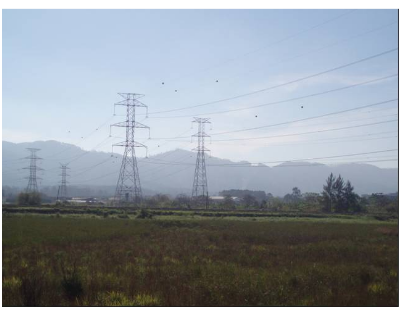
\includegraphics[width=0.5\textwidth]{Estrutura_linha.png}			
 	\caption{Instalação típica de uma linha de transmissão}		
 	\label{img:Estrutura_Linha}	
 	\source{\cite{rangel2009sistema}}		
 \end{figure}
 
 Segundo \cite{rangel2009sistema}, as rotinas de inspeção de linhas de transmissão se dão principalmente por dois métodos: inspeções por aeronaves e inspeções terrestres.
 A inspeção realizada por aeronaves, se dá tipicamente com o uso de helicópteros, que executam voos em baixa altitude, extremamente próximos das linhas de transmissão. 
 
 Em alguns casos as condições climáticas podem dificultar o procedimento de inspeção e controle da aeronave, além do risco inerente da atividade para os tripulantes, principalmente devido ao fato de que as aeronaves tipicamente operam na região de “homem-morto”, uma zona de altura que representa perigo para os operadores a bordo das aeronaves em caso de uma queda.
 
  \begin{figure}[h!]												
  	\centering												
  	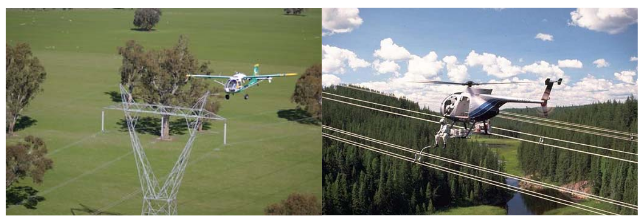
\includegraphics[width=0.5\textwidth]{Inspecao_metodos.png}			
  	\caption{Inspeção em linhas de transmissão por veículos aéreos tripulados.}		
  	\label{img:Inspecao_metodos}	
  	\source{\cite{rangel2009sistema}}		
  \end{figure}
 
 A inspeção por vias terrestres possui uma grande dificuldade devido à dependência do terreno do local, o qual pode ser de difícil acesso devido às características geográficas.Diversos fatores tornam a inspeção de linhas de transmissão um procedimento não só perigoso, mas também altamente custoso. 
 
 Segundo \cite{cinematicajuliana} as principais desvantagens dos meios convencionais de inspeção de linhas de transmissão são os riscos de acidentes, devido a periculosidade do procedimento de inspeção; o alto custo, uma vez que é necessário a locação e deslocamento de equipamentos específicos para o transporte e inspeção das linhas de transmissão; a alta dependência das condições climáticas e geográficas, uma vez que se torna muito difícil realizar rotinas de inspeção em tempos chuvosos ou em locais de difícil acesso.
 
 Outra grande desvantagem dos procedimentos de inspeção definida por \cite{cinematicajuliana} é justamente a necessidade de uma mão de obra qualificada para realização destes procedimentos. Se estes procedimentos de inspeção de linha de transmissão fossem realizados em linhas desenergizadas, o processo seria bem mais simples e rápido, porém existem diversos problemas atrelados ao fato de que existem inúmeras cargas consumidoras que necessitam da energia elétrica gerada.


%--------- NEW SECTION ----------------------
\section{Organização do \thetypework}
\label{section:organizacao}
O documento está organizado em cinco capítulos, seguindo a seguinte estrutura:

\textbf{Capitulo 1 - Introdução}: Faz a contextualização do âmbito no qual a pesquisa proposta
está inserida. Apresenta, portanto, a problemática, objetivos e como este projeto Theoprax de conclusão de curso está estruturado


\textbf{Capítulo 2 - Referencial Teórico}: Apresenta a base teórica necessária para o desenvolvimento do projeto.

\textbf{Capítulo 3 - Metodologia}: Define o método adotado para o desenvolvimento do projeto, explicitando seu fluxo de atividades e premissas necessárias para aplicar a metodologia.

\textbf{Capítulo 4 - Desenvolvimento}: Exibe os procedimentos realizados e resultados obtidos através de testes, unitários e integrados, durante o desenvolvimento do projeto.

\textbf{Capítulo 5 - Conclusão}: Apresenta as conclusões, contribuições e algumas sugestões de atividades de pesquisa a serem desenvolvidas futuramente.



    \chapter{Fundamentação Teória}
\label{chap:concep}
O termo robô vem da palavra tcheca robota que tem como uma das possíveis traduções “trabalhador forçado” e ganhou o significado atual após o escritor tcheco Karel Capek (1809 - 1938), na sua obra de ficção científica “R.U.R. Rossumovi Univerzální Roboti”, associar o termo às máquinas criadas pelo personagem principal para servi-lo. Mas a ideia de algo que desenvolva atividades de maneira autônoma é apresentada ao mundo muito tempo antes. \cite{aristoteles1985traduccao} diz: “Se cada instrumento pudesse realizar sozinho a sua tarefa, obedecendo ou antecipando a nossa vontade, [...] os feitores não precisariam de servos, nem os senhores de escravos.” 

Diversas obras da ficção retratam diferentes tipos de robôs criados de forma a reproduzir comportamentos semelhantes aos de um ser humano. Com o passar do tempo, juntamente com o avanço tecnológico nas áreas da eletrônica, mecânica e informática, a construção dessas máquinas se tornou possível. A indústria observou nos robôs, o potencial para automatizar e otimizar as linhas de processo, onde atividades que pudessem demandar mais tempo se fossem executadas por seres humanos, seriam executadas de forma muito mais rápida e precisa com a utilização de máquinas programadas e autônomas, aumentando a produção.

A \cite{iso2012} define um robô como “mecanismo programável atuado em dois ou mais eixos com um grau de autonomia, movendo-se dentro do seu ambiente, para executar tarefas pretendidas”. É resultado da integração de componentes como: Sensores; atuadores; unidade de controle; unidade de potência e manipulador mecânico. Sensores são os componentes que fornecem parâmetros sobre o ambiente em que o robô se encontra e sobre o comportamento do próprio sistema robótico. Já os atuadores são os dispositivos que movimentam as partes, quando convertem energia elétrica, hidráulica ou pneumática em mecânica. A energia necessária para o funcionamento dos atuadores é fornecida pela unidade de potência.

O gerenciamento dos parâmetros necessários para que o robô realize suas tarefas é de responsabilidade da unidade de controle. De onde também são emitidos os comandos para a movimentação. O manipulador mecânico é o conjunto de componentes estruturais do robô, elos ou links, conectados entre si por articulações comumente denominadas de juntas. Graus de liberdade, segundo \cite{romanorobotica} “É o número mínimo de variáveis independentes de posição que precisam ser especificadas para se definir inequivocamente a localização de todas as partes de um mecanismo”.

\section{Cinemática}\label{sec:cinem}
A cinemática é o ramo da física que descreve o movimento de um corpo, determinando características como posição, velocidade e aceleração. Na robótica, o estudo cinemático resulta em um conjunto de equações que caracterizam o movimento do robô, a complexidade da solução varia com a quantidade de graus de liberdade que esse robô tem. Em um manipulador mecânico composto por links que são conectados por juntas, cada conjunto link-junta caracteriza um grau de liberdade. Dessa maneira, um robô com $n$ conjuntos link-junta tem $n$ graus de liberdade, sendo o primeiro link a base de sustentação do robô no mundo e o último, onde está a seu end-effector.

\subsection{Cinemática Direta}\label{sec:cinem_dir}
A cinemática direta é a solução para a movimentação de um robô com cálculo da posição e orientação do end-effector a partir de dadas posições das juntas. A notação de Denavit-Hartenberg é uma ferramenta utilizada para coordenar a descrição cinemática de sistemas mecânicos articulados com $n$ graus de liberdade.

\begin{figure}[h!]												
	\centering												
	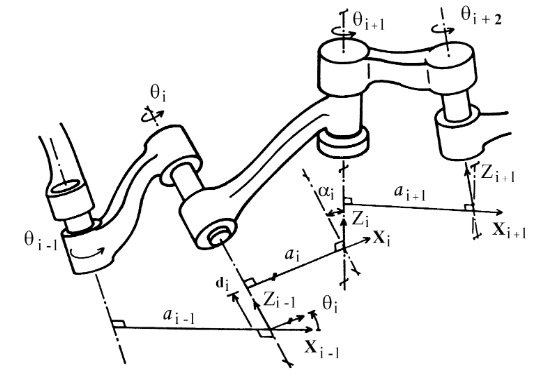
\includegraphics[width=0.5\textwidth]{denavit.PNG}			
	\caption{Parâmetros de Denavit-Hartenberg}		
	\label{img:denavit}	
	\source{\cite{romanorobotica}}		
\end{figure}

A figura mostra dois \textit{links} ligados por uma junta de superfícies deslizantes uma sobre a outra. Um eixo de uma junta estabelece a conexão de dois \textit{links}. Segundo \cite{romanorobotica}, os eixos das juntas devem ter duas normais conectadas a eles, uma para cada um dos \textit{links}. Assim a posição relativa destes dois \textit{links} conectados ($i-1$ e $i$) é dada por $d_{i}$, que é a distância medida ao longo do eixo da junta entre suas normais. O ângulo de junta $\theta_{i}$ entre as normais é medido em um plano normal ao eixo da junta. Dessa forma, $d_{i}$ e $\theta_{i}$ são a distância e o ângulo entre os \textit{links} adjacentes. Determinam a posição relativa de \textit{links} vizinhos.

Um \textit{link} pode apenas ser conectado a dois outros \textit{links} ($i-1$ e $i+1$). Assim, dois eixos de juntas são estabelecidos em ambos terminais de conexão. Os \textit{links} mantém uma configuração fixa entre as juntas e podem ser caracterizados pelos parâmetros $a_{i}$ e $\alpha_{i}$. O parâmetro $a_{i}$ é a menor distância medida ao longo da normal comum entre os eixos da junta, chamado de comprimento de \textit{twist}, já o $\alpha_{i}$ é o ângulo de \textit{twist}. Esses quatro parâmetros determinam a estrutura do \textit{link}, parâmetros da junta e a posição relativa aos \textit{links} vizinhos.

A representação de Denavit-Hartenberg \cite{denavit1955kinematic} tem como resultado uma matriz 4 x 4 representando cada sistema de coordenadas do \textit{link} na junta em relação ao \textit{link} anterior. Essa matriz é obtida através do produto das transformações: Translação de uma distância $d_{i}$ ao longo do eixo $Z_{i-1}$ para trazer os eixos $X_{i-1}$ e $X_{i}$ na coincidência; Rotação no eixo $Z_{i-1}$ de um ângulo $\theta_{i}$ para alinhar os eixos $X_{i-1}$ e $X_{i}$; Translação ao longo do eixo $X_{i}$ de uma distância $a_{i}$ para trazer as duas origens na coincidência; Rotação do eixo $X_{i}$ um ângulo $\alpha_{i}$ para trazer os dois sistemas de coordenadas na coincidência. Isso resulta na matriz de transformação homogênea $^{i-1}A_{i}$.

\begin{equation}
^{i-1}A_{i}=T_{z,d} T_{z,\theta} T_{x,a} T_{z,\alpha}
\end{equation}
\begin{equation}
^{i-1}A_{i}=\begin{bmatrix}
1 & 0 & 0 & 0\\ 
0 & 1 & 0 & 0\\ 
0 & 0 & 1 & d_{i}\\ 
0 & 0 & 0 & 1
\end{bmatrix}\begin{bmatrix}
cos\theta_{i} & -sin\theta_{i} & 0 & 0\\ 
sin\theta_{i} & cos\theta_{i} & 0 & 0\\ 
0 & 0 & 1 & 0\\ 
0 & 0 & 0 & 1
\end{bmatrix}\begin{bmatrix}
1 & 0 & 0 & a_{i}\\ 
0 & 1 & 0 & 0\\ 
0 & 0 & 1 & 0\\ 
0 & 0 & 0 & 1
\end{bmatrix}\begin{bmatrix}
1 & 0 & 0 & 0\\ 
0 & cos\alpha_{i} & -sin\alpha_{i} & 0\\ 
0 & sin\alpha_{i} & cos\alpha_{i} & 0\\ 
0 & 0 & 0 & 1
\end{bmatrix}\end{equation}
\begin{equation}
^{i-1}A_{i}=\begin{bmatrix}
cos\theta_{i} & -cos\alpha_{i}sin\alpha_{i} & sen\alpha_{i}sin\theta_{i} & a_{i}cos\theta_{i}\\ 
sin\theta_{i} & cos\alpha_{i}cos\theta_{i} & -sin\alpha_{i}cos\theta_{i} & a_{i}sin\theta_{i}\\ 
0 & sin\alpha_{i} & cos\alpha_{i} & d_{i}\\ 
0 & 0 & 0 & 1
\end{bmatrix}
\end{equation}

\subsection{Cinemática Inversa}\label{sec:cinem_inv}
Segundo \cite{fu1987robotics} os robôs estão em um espaço onde o objeto a ser manipulado tem sua posição expressa no sistema de coordenadas do ambiente. Com o objetivo de controlar a posição e orientação do \textit{end-effector} do robô, a solução da cinemática inversa é mais adequada. A cinemática inversa consiste em, partindo de uma posição e orientação desejada, calcula-se as posições das juntas para que o robô alcance esse objetivo, é o processo inverso da cinemática direta. 

Há de se observar que a cinemática inversa pode ou não ter solução, caso a posição de interesse esteja fora do espaço de trabalho do robô, não há posições de juntas que execute a tarefa. Nos momentos em que a posição desejada pode ser alcançada, podem existir mais de uma solução. Um ponto importante na solução da cinemática inversa é, quando há mais de uma solução deve-se atentar para qual delas é a melhor opção, levando em consideração o ambiente em que o robô se encontra, principalmente os obstáculos à sua volta. A demanda energética para a execução dos possíveis movimentos e o esforço qual as juntas serão submetidas nesta ação, é crucial para o planejamento da movimentação do robô.


\section{Modelagem Cinemática de um Braço Planar}\label{sec:brac_plan}
O robô ELIR tem na sua estrutura, braços que se movimentam apenas em dois eixos, $x$ e $z$, através da atuação de duas juntas, podendo assim ser modelado cinematicamente como um braço planar do tipo RR. A figura a seguir mostra um exemplo desse braço, RR por ter duas juntas rotativas, que se movimenta no plano $x-y$:

\begin{figure}[h!]												
	\centering												
	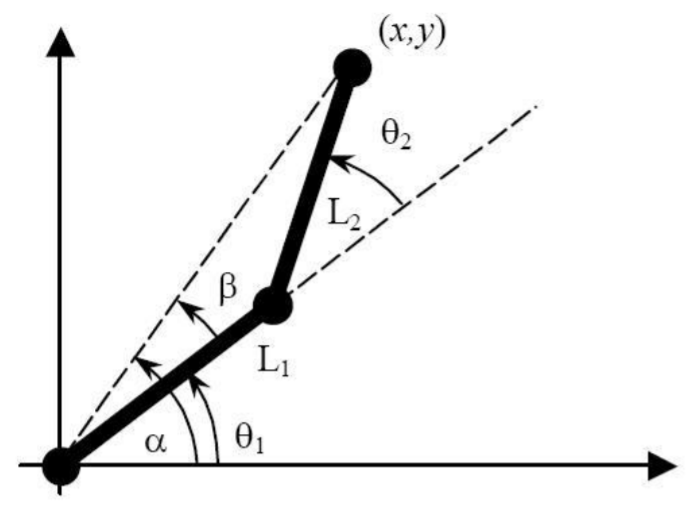
\includegraphics[width=0.5\textwidth]{planar_rr.PNG}			
	\caption{Braço planar do tipo RR}		
	\label{img:planar}	
	\source{\cite{cinem_inv}}		
\end{figure}

Usando a análise da cinemática direta, consegue-se determinar a posição do \textit{end-effector} com base nos ângulos $\theta_{1}$ e $\theta_{2}$ e nas dimensões $L_{1}$ e $L_{2}$. Logo tem-se que:
\begin{equation}
x=L_1cos{(\theta_1)}+L_2cos{(\theta_1 + \theta_2)}
\end{equation}
\begin{equation}
y=L_{1}sen{(\theta_1)}+L_{2}sen{(\theta_1 + \theta_2)}
\end{equation}
Aplicando a lei dos cossenos ao triângulo formado pelo braço e pela linha entre a origem do braço e o seu \textit{end-effector} obtém-se: 
\begin{equation}
\theta_2=\pm arccos{\frac{(x^2+y^2-(L_1)^2-(L_2)^2)}{2L_1L_2}}
\end{equation}
Para determinar o $\theta_{1}$ considera-se a relação trigonométrica:
\begin{equation}
tan{(A - B)}=\frac{tan(A)-tan(B)}{1+tan(A) tan(B)}
\end{equation}
e tomando:
\begin{equation}
tan(\beta)=\frac{L_2 sin\theta_2}{L_1 + L_2 cos\theta_2}
\end{equation}
tem-se que:
\begin{equation}
\theta_1 = arctan[\frac{y(L_1 + L_2 cos\theta_2)-xL_2 sin\theta_2}{x(L_1 + L_2 cos\theta_2)-yL_2 sin\theta_2}]
\end{equation}
Assim é possível fazer a solução da cinemática inversa para um braço planar RR.

\section{Desenvolvimento de Robôs}\label{sec:desen_robo}
Para o desenvolvimento de sistemas robóticos, é necessária a integração de vários dispositivos, assim sendo necessário utilizar ferramentas e tecnologias que poupem tempo no desenvolvimento, de forma a facilitar o processo de comunicação entre as diversas camadas de abstração. 
As camadas de abstração se referenciam ao alto e baixo nível da máquina, onde baixo nível é uma referência para aplicações mais simples, que estão mais próximas da linguagem da máquina, como por exemplo aplicação de comunicação somente via \textit{bytes}. Um exemplo de um elemento que está numa camada de abstração de alto nível é uma Interface Homem-Máquina , onde o usuário consegue interagir com a máquina diretamente, sem ter que necessariamente entender o seu funcionamento interno.

\subsection{\textit{Framework}}\label{sec:framework}
Em ambientes computacionais, a utilização de ferramentas para realização de atividades e desenvolvimento de soluções é de extrema importância. Estas ferramentas podem ser softwares específicos para execução de uma determinada atividade ou \textit{frameworks}.	
Segundo \cite{maxwel_framework} “\textit{Frameworks} são estruturas de classes que constituem implementações incompletas que, estendidas, permitem produzir diferentes artefatos de software”. Os \textit{frameworks} em geral permitem o desenvolvimento de soluções computacionais baseadas em determinadas funcionalidades, seguindo uma estrutura definida pelo \textit{framework}. De acordo com \cite{maxwel_framework} os \textit{frameworks} definem uma arquitetura para um conjunto de subsistemas, dando os construtores necessários para a sua criação.

A principal característica de um \textit{framework} é a sua capacidade de reutilização, afinal a sua utilização permite que diversos conjuntos de produtos possam ser gerados partindo de uma única estrutura que possua os conceitos mais gerais.
Segundo \cite{maxwel_framework} \textit{frameworks} podem ser classificados em dois tipos principais: \textit{Frameworks} de Aplicações Orientado a Objetos e \textit{Frameworks} de Componente.
Os \textit{frameworks} orientados a objetos geram famílias de aplicações orientadas a objetos e seus pontos de extensão são definidos como classes abstratas ou interfaces, onde se estendem por cada instância da família de aplicações.
Para \textit{frameworks} de componentes, o suporte é previsto para componentes que sigam um determinado modelo, possibilitando que as instâncias destes componentes sejam acopladas ao \textit{framework}. Também são estabelecidas as condições necessárias para que um componente seja executado, regulando a sua interação entre as instâncias de outros componentes.

Os \textit{frameworks} utilizados para robótica, são extremamente importantes, pois o uso de suas ferramentas possibilita o desenvolvimento e criação das soluções computacionais e códigos necessários para cada funcionalidade de um robô, de forma que o funcionamento delas em conjunto seja otimizado pela natureza do \textit{framework} de realizar a compatibilização entre as estruturas.

\subsection{Simulação}\label{sec:simula}

Em sistemas complexos, onde diversas variáveis definem o seu funcionamento, e por consequência as suas respostas a determinados estímulos, torna-se extremamente difícil e irresponsável executar a sua fabricação antes de realizar uma validação prévia de seu funcionamento.

Este tipo de procedimento de análise prévia do comportamento de um sistema é chamado de simulação. De acordo com \cite{definicao_de_simulacao} "Simulação refere-se a uma ampla coleção de métodos e aplicações para imitar o comportamento do sistema real, por meio de um computador com um \textit{software} apropriado". Diversos tipos de sistemas se utilizam da ferramenta de simulação para validar previamente o funcionamento de projetos.

O processo de utilização de uma simulação consiste em basicamente recriar o sistema em questão em um ambiente computacional e então são fornecidas as entradas para o sistema, as rotinas de tratamento destas entradas e por fim as saídas da simulação.

\begin{figure}[h!]												
	\centering												
	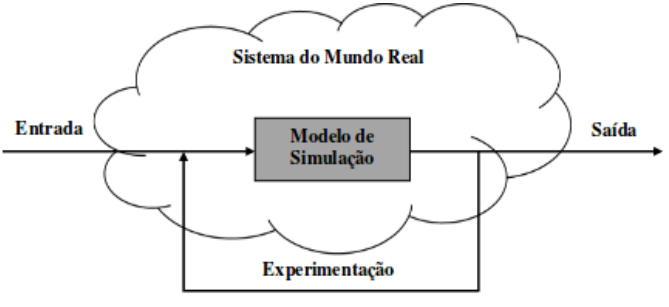
\includegraphics[width=0.5\textwidth]{simulation.PNG}			
	\caption{Diagrama de funcionamento de um processo de simulação}		
	\label{img:simulation}	
	\source{\cite{definicao_de_simulacao}}		
\end{figure}


Em sistemas robóticos, uma ferramenta extremamente útil e bastante utilizada, é a simulação. Segundo \cite{artigo_sobre_simulacao} 
\begin{quote}
“Quando se trabalha com robótica, o uso de uma simulação é de importância significante. Por um lado, ela permite a validação de diferentes alternativas durante o design do sistema robótico, levando assim, a melhores decisões e preservação de custos. Por outro lado, auxilia o processo de desenvolvimento de \textit{software}, disponibilizando uma reposição para robôs que não estejam em mãos”.
\end{quote}

Através do uso de \textit{softwares} de simulação é possível criar uma representação computacional não só o modelo físico de um robô, mas também os parâmetros referentes à objetos do ambiente no qual o mesmo será posto em funcionamento. A avaliação prévia da execução das tarefas e do funcionamento do robô, permite a observação do comportamento do sistema em determinadas situações, facilitando assim, a tomada de decisões mais efetivas no processo de desenvolvimento do protótipo real. 

\subsection{Odometria}\label{sec:odom}
A odometria consiste no cálculo para estimar a mudança de posição do robô no tempo, onde isso pode se dar por meio de diversos dispositivos que possibilitem o cálculo de deslocamento. Onde segundo \cite{ben2018robotic}, "Odometria - a medição da distância - é um método fundamental usado por robôs para navegação". A medição de tempo é fácil utilizando o \textit{clock} interno do computador embutido. Medir velocidade é mais difícil: em alguns robôs educacionais utilizam codificadores são usados para contar as rotações da rodas, enquanto em outros a velocidade é estimada das propriedades dos motores.

No caso da análise de deslocamento do robô na linha por meio de roldanas, o movimento é caracterizado como linear, já que o deslocamento ocorre em somente uma direção, analogamente a odometria utilizada é a linear, onde o deslocamento pode ser calculado simplesmente pela equação \ref{eq:deslocamento} onde $s$ representa o espaço caminhando, $v$ a velocidade e $t$ o tempo. 

\begin{equation}\label{eq:deslocamento}
s = v*t
\end{equation}

Utilizando o medidor de tempo interno do computador embutido nos sistemas robóticos, pode se calcular a variação de espaço para um tempo muito pequeno, onde esses pequenos incrementos são somados ou subtraídos para encontrar o deslocamento do robô.

A velocidade de deslocamento das roldanas pode ser encontrada utilizando a equação \ref{eq:vel} com as informações do raio da roldana $r$ e a sua velocidade de giro $w$ em radianos por segundo. A informação da velocidade de giro da roldana geralmente é extraída dos servomotores utilizados para tração.

\begin{equation}\label{eq:vel}
v = 2\pi*r*w
\end{equation}

O cálculo da odometria por meio da velocidade das rodas é denominado no âmbito da robótica como odometria de roda, \textit{wheel odometry} em inglês, porém, outras técnicas são utilizadas, já que existem diversos tipos de deslocamento diferentes. Outro tipo aplicação muito encontrada é a odometria visual, que segundo \cite{nister2004visual} "Odometria Visual (OV) é o processo de estimação do deslocamento de um agente (ex: veículo, humano e robô) utilizando a entrada de uma ou múltiplas câmeras conectadas a ele". Os domínios da aplicação incluem robótica, realidade aumentada, automotiva e 'computadores vestíveis'.

\subsection{Gestão de Energia}\label{sec:gestao}
O conceito de gestão de energia se dá pela forma como a energia elétrica é utilizada em um sistema composto de diversos dispositivos elétricos e eletrônicos. Para sistemas robóticos, este conceito representa um fator importante para garantir uma operação autônoma de qualidade. Os robôs quando nesse tipo de operação, geralmente não dispõem de uma fonte de energia constante, e portanto, são geralmente alimentados por baterias e tendo interação por meio de conexões sem fio. 

O uso de diversos dispositivos eletrônicos de baixo consumo energético, como sensores e interfaces microcontroladas, podem não se mostrar um problema para um curto período de operação, porém, para maximizar o tempo da atividade exercida pelo robô, é necessário encontrar uma forma eficiente de gerir a operação dos dispositivos conectados na rede de alimentação. Segundo \cite{katiraei2006power} 
\begin{quote}
“Gestão de energia é um conceito importante em redes de sensores, porque uma estrutura de energia cabeada geralmente não está disponível e um conceito óbvio é utilizar a energia disponível da bateria de forma eficiente”. 
\end{quote}	
Quanto mais atividades diferentes o robô desempenha maior será a demanda de energia entre os dispositivos interconectados, isso faz com que seja necessário que os desenvolvedores busquem uma forma de otimizar o custo de energia individual das atividades e do fluxo de operação como um todo. Os diversos dispositivos utilizados em sistemas robóticos fazem com que o mesmo se utilize de diferentes níveis de tensão e corrente, já que comumente, os dispositivos utilizados são comerciais, e devido às diferenças das suas características e parâmetros, definidos por empresas diferentes, responsáveis pela produção e fabricação das ferramentas, é necessário que a gestão de energia leve em consideração a compatibilidade entre diferentes dispositivos.

\subsection{Conceito de segurança e Integridade}\label{sec:segur_inte}
Em diversas áreas, é comum a verificação das condições antes da execução de atividades, a aviação é um grande exemplo de uso desse conceito. Neste seguimento, o \textit{checklist} é utilizado toda vez antes de um avião decolar, assim é possível verificar se os sistemas vitais para o vôo estão em ordem. O principal objetivo dessa ação é identificar os riscos que existem para o cumprimento da atividade.

Para que um dispositivo robótico execute as tarefas para as quais ele foi desenvolvido, deve-se verificar se os seus sistemas, como um todo, e os componentes individualmente, estão em condições de funcionamento, garantindo assim a integridade do sistema como um todo. Essa análise deve ser feita levando em conta a importância de cada sistema e de cada componente desses sistemas, a fim de aumentar a capacidade de operação em condições adversas do robô. Podem existir sistemas que, mesmo quando não estão operando adequadamente, não comprometem a execução da missão do robô.

\subsection{Comunicação em sistemas robóticos}\label{sec:comm_sis}
Dispositivos eletrônicos são capazes de realizar transmissão de dados, afinal, a interconexão entre eles é de extrema importância em sistemas em que existam diversos dispositivos responsáveis por funções distintas. Dispositivos que se comunicam entre si, são capazes de criar uma rede em todo o sistema, permitindo um aumento na confiabilidade das funções do sistema, através da troca de informações de parâmetros que venham a ser importantes para o funcionamento do sistema como um todo.

Para que os dispositivos possam se comunicar entre si, os mesmos adotam o que se chama de protocolos de comunicação. Protocolos de comunicação são arquiteturas que estabelecem a troca de dados entre dispositivos eletrônicos. Os dispositivos comerciais possuem diferentes tipos de protocolos de comunicação e por isso, torna-se extremamente importante se atentar a qual protocolo utilizar durante a conceituação de um projeto que se tenha a necessidade da interconexão de dispositivos.

Uma das formas mais comuns de se realizar a transmissão de dados entre dispositivos embarcados é a comunicação serial. \cite{livro_sistemas_embarcados} define a comunicação serial como um envio de \textit{bits} de forma serial, similar a uma fila. Possuindo dois canais principais: o canal $TX$ para envio e o canal $RX$ para recebimento. Dentro desse processo de comunicação alguns parâmetros devem ser levados em conta, como a taxa de transmissão de dados (\textit{BaudRate}); bits de paridade, para assegurar que o número de bits no campo de dados é par ou ímpar; bits de parada para indicar o início ou fim de uma comunicação.

Outro meio de comunicação muito utilizado é o USB (\textit{Universal Serial Bus}), criado com a intenção de tornar a comunicação serial mais simplificada e com uma taxa de transmissão muito mais elevada. Os cabos conectores USB possuem geralmente quatro fios condutores, sendo dois deles para alimentação e dois outros cabos de dados. Os cabos de dados são nomeados como D+ e D-, onde a comunicação entre os dispositivos se dá pela variação de tensão entre estes dois sinais.
Dentro de ampla complexidade como um robô, onde diversos dispositivos necessitam estar trocando informações, a utilização de protocolos de comunicação serial se tornam extremamente importantes para a garantia da confiabilidade na execução de tarefas e operações.

    \chapter{Materiais e Métodos}
\label{chap:mat}
Esta seção destaca o que é necessário para construção do projeto, contendo a lista de materiais, especificação dos componentes, funcionalidades, modelo esquemático de comunicação e de alimentação.


\section{Estrutura analítica do protótipo}
\label{ssec:pbs}
De forma sistemática o projeto ELIR foi dividido em 6 subsistemas, caraterizando a estrutura analítica do projeto (Figura \ref{fig:pbselir}) em:

\begin{itemize}
	\item \textit{perception}
	\item \textit{actuation}
	\item \textit{power management}
	\item \textit{processing system}
	\item \textit{detection}
	\item \textit{software}
\end{itemize}

Os cinco iniciais subsistemas estão mais ligados as condições físicas de hardware do que o subsistema \textbf{software}, porém as implicações de software também devem ser consideradas em cada um destes susbsistemas.

O susbistema \textbf{software} foi idealizado a partir das funcionalidades desenvolvidas  para a solução final do projeto, e estão descriminadas na secção \ref{sec:espf}.

%----- figure --------------------------------------
\begin{figure}[!htb]
	\centering
	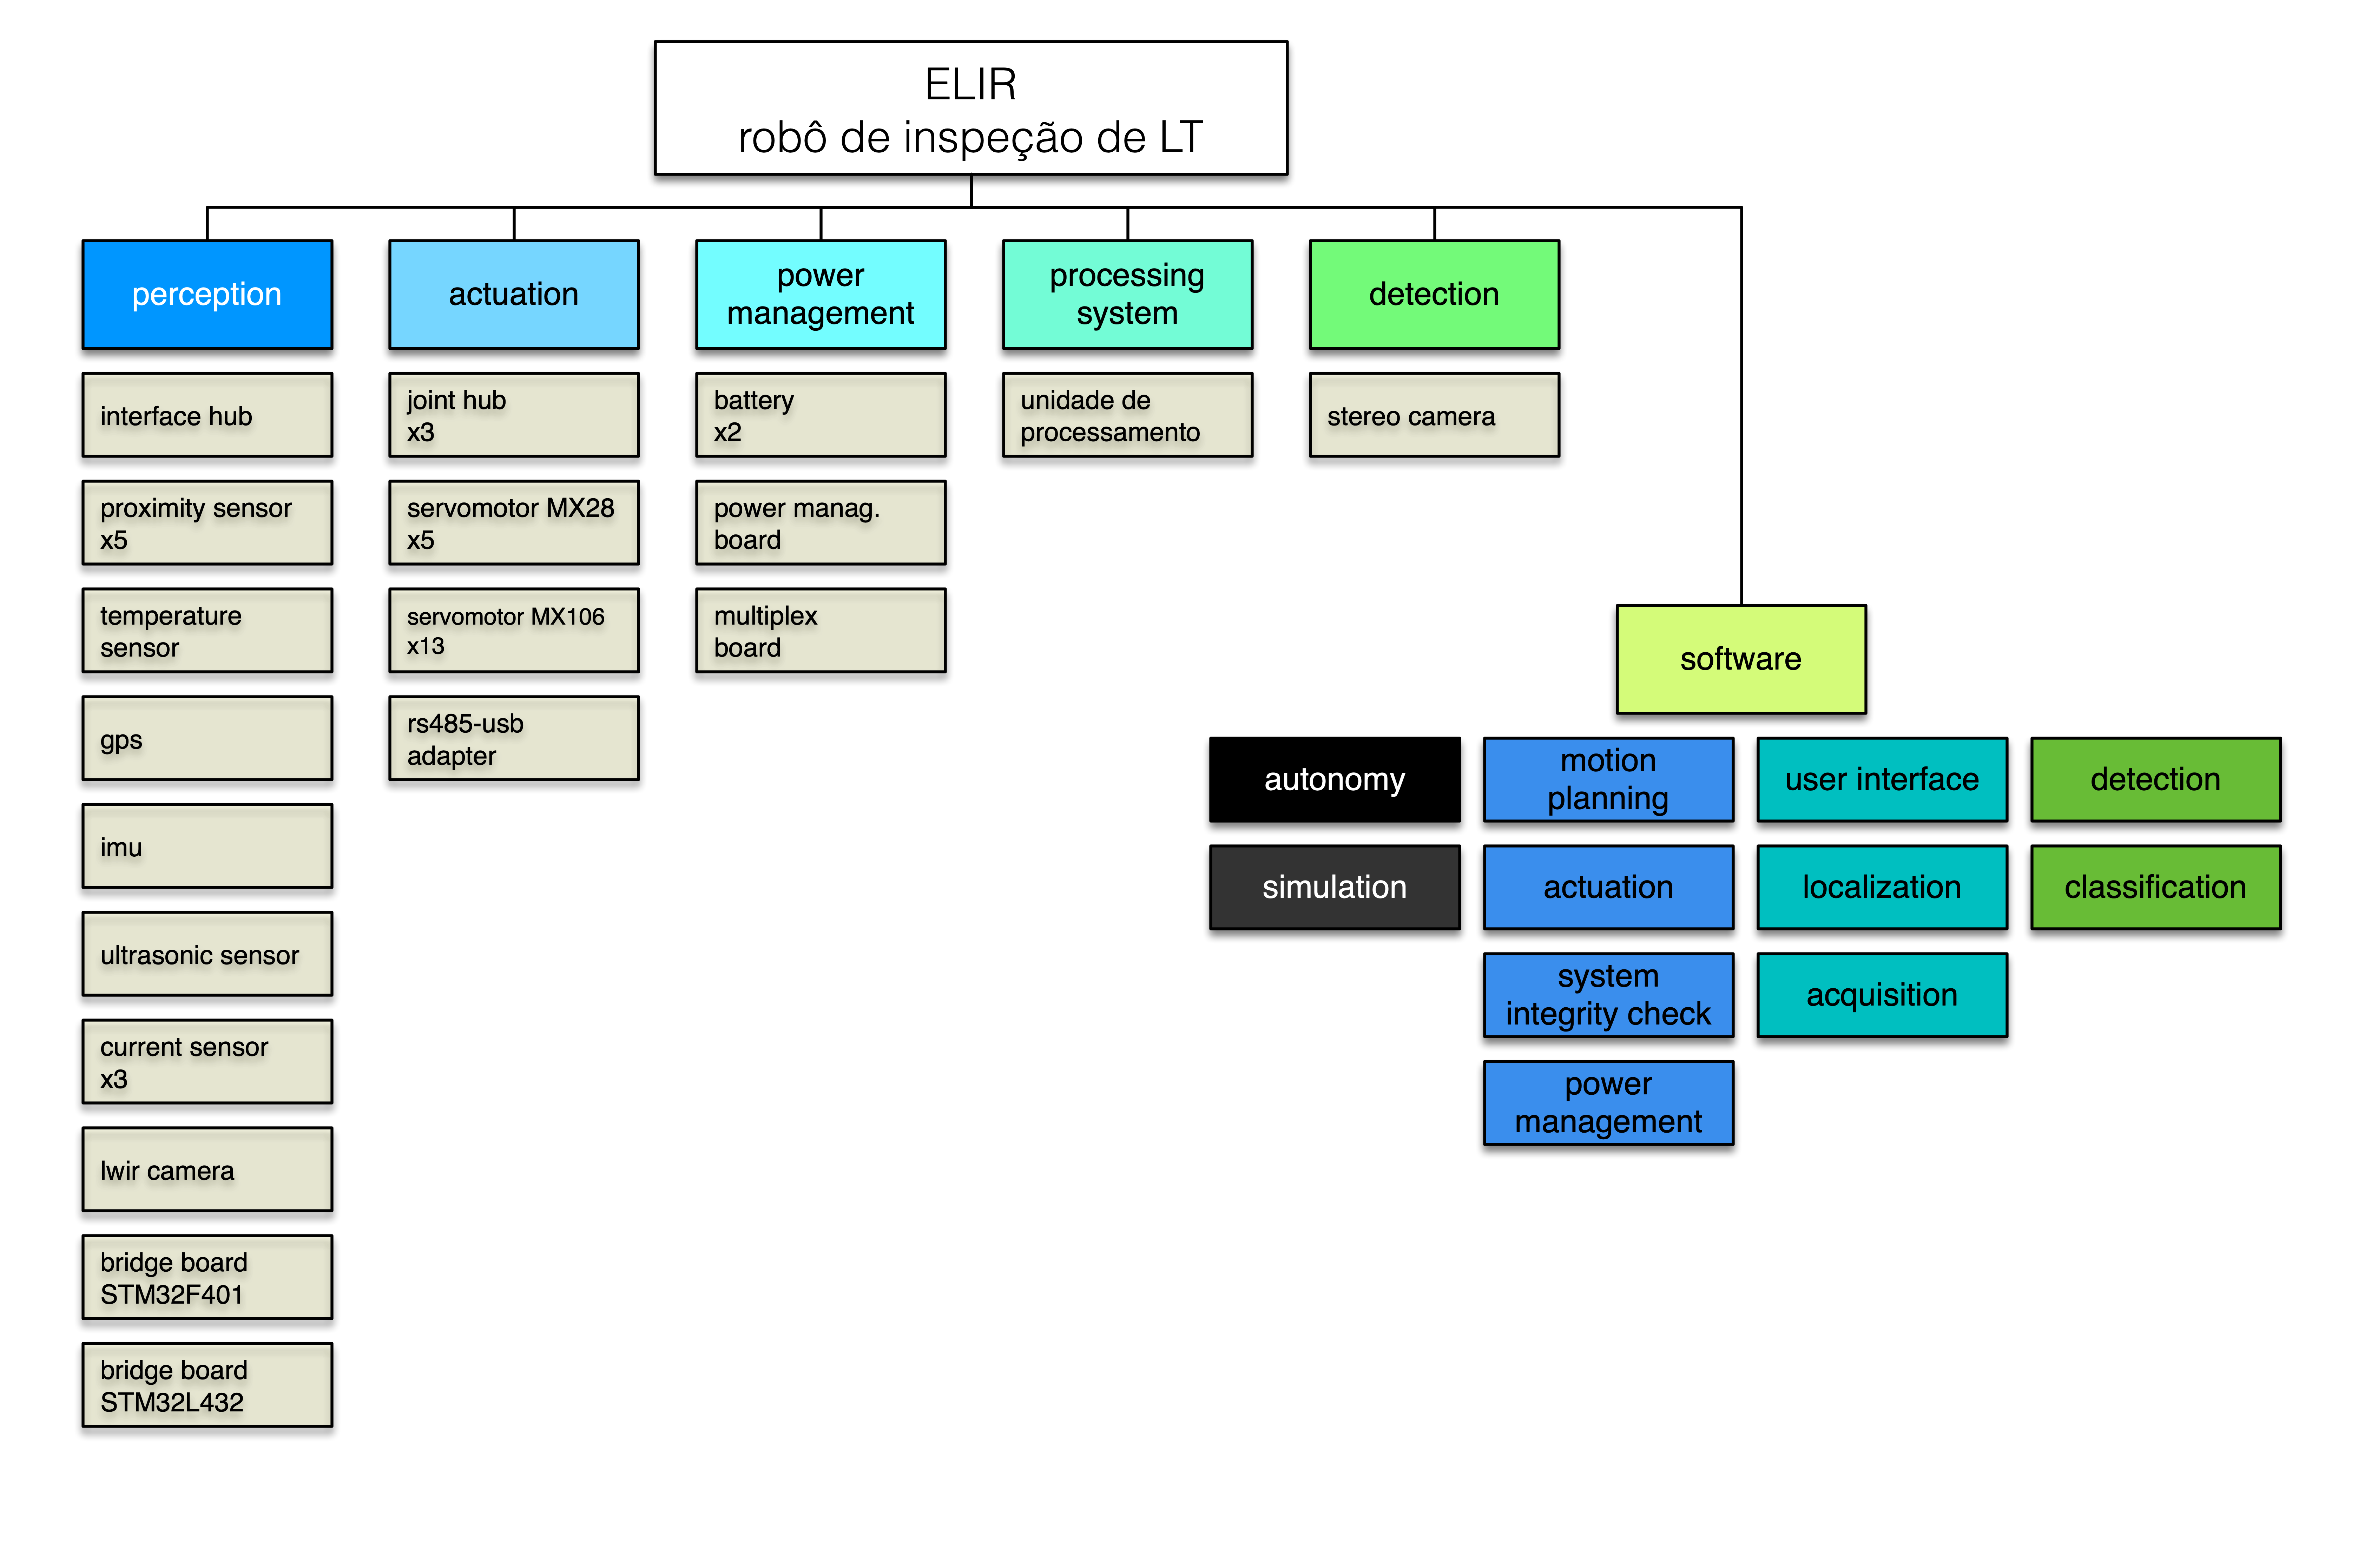
\includegraphics[scale=0.6]{Figures/pbselir.png}
	\caption{Esturutura analítica do sistema.}
	%\legend{Fonte: os autores}
	\label{fig:pbselir}
\end{figure}
%---------------------------------------------------

%fazer comentário sobre os subsistemas

A relação final dos componentes do sistema robótico encontra-se no Apêndice \ref{Append:bom}.

%--------- NEW SECTION----------------------
\section{Especificação dos componentes}
\label{sec:espc}
Serão detalhados os componentes utilizados para confecção do protótipo, sendo eles físicos ou digitais.

\subsection{Estrutura analítica do protótipo}
\label{ssec:pbs}



\subsection{Lista de componentes}
\label{ssec:list}

\subsection{Servomotores}
Os servomotores são responsáveis pelo atuação do robô, realizando os movimentos das juntas dos braços e das garras, além de atuarem as rodas que deslocam o robô na linha. São utilizados os servomotores da Robotis, \textit{Dynamixel} MX-106R e MX-28. Esses motores foram escolhidos pois apresentam drivers prontos para o \textit{ROS} , que possibilitam uma integração mais fácil com as ferramentas de controle, apresentando bom torque, peso reduzido e fácil integração para controle conjunto.

\begin{table}[h!]
	\begin{tabular}{ll}
		
		\multicolumn{2}{c}{Robotis Dynamixel MX-28R}                                            \\ \hline
		Peso (g)                     & 153                                                      \\ \hline
		Dimensões (mm)               & 40.2 x 65.1 x 46                                         \\ \hline
		Torque (N.m)                 & 8.0 (em 11.1V), 8.4 (em 12V) e 10.0 (em 14.4V)           \\ \hline
		Temperatura de operação (ºC) & -5 até +80                                               \\ \hline
		Tensão de operação (V)       & 10 até 14.8 (Tensão recomendada: 12V)                    \\ \hline
		Baud rate                    & 8000bps até 4.5Mbps                                      \\ \hline
		Protocolo de comunicação     & RS485                                                    \\ \hline
		Resolução                    & 0.088º                                                   \\ \hline
		ID                           & 254 ID (0 até 253)                                       \\ \hline
		Feedback                     & Posição, temperatura, carga, tensão de alimentação, etc. \\ \hline
	\end{tabular}
	\caption{Especificações Motor Robotis\textit{ Dynamixel} MX-28R  }
\end{table}

 

\begin{figure}[h!]												
	\centering												
	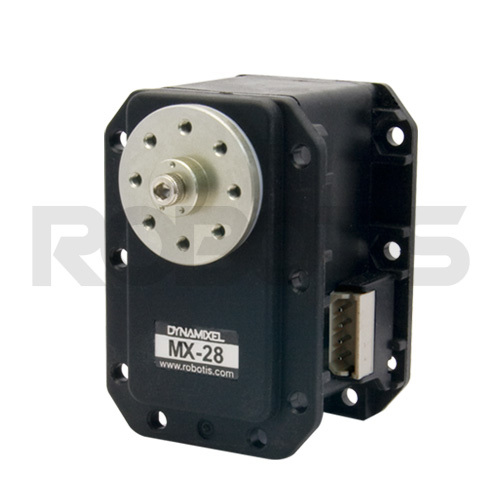
\includegraphics[width=0.25\textwidth]{mx-28r.jpg}				
	\caption{Motor Robotis\textit{ Dynamixel} MX-28R.}		
	\label{img:mx28}
	\source{\cite{robotis_site}}												
\end{figure}

\begin{figure}[h!]												
	\centering												
	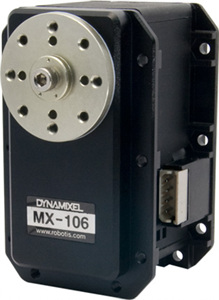
\includegraphics[width=0.25\textwidth]{mx-106r.jpg}				
	\caption{Motor Robotis\textit{ Dynamixel} MX-106R}		
	\label{img:mx106}	
	\source{\cite{robotis_site}}		
\end{figure}

\begin{table}[h!]
	\begin{tabular}{ll}
	
		\multicolumn{2}{c}{Robotis Dynamixel MX-28R}                                            \\ \hline
		Peso (g)                     & 153                                                      \\ \hline
		Dimensões (mm)               & 40.2 x 65.1 x 46                                         \\ \hline
		Torque (N.m)                 & 8.0 (em 11.1V), 8.4 (em 12V) e 10.0 (em 14.4V)           \\ \hline
		Temperatura de operação (ºC) & -5 até +80                                               \\ \hline
		Tensão de operação (V)       & 10 até 14.8 (Tensão recomendada: 12V)                    \\ \hline
		Baud rate                    & 8000bps até 4.5Mbps                                      \\ \hline
		Protocolo de comunicação     & RS485                                                    \\ \hline
		Resolução                    & 0.088º                                                   \\ \hline
		ID                           & 254 ID (0 até 253)                                       \\ \hline
		Feedback                     & Posição, temperatura, carga, tensão de alimentação, etc. \\ \hline
	\end{tabular}
	\caption{Especificações Motor Robotis\textit{ Dynamixel} MX-106R  }
\end{table}



\subsection{Placa de Gerenciamento de Energia (Power Management)}
A placa de gerenciamento de energia é responsável pela distribuição de corrente e de tensão para todos os componentes elétricos e eletrônicos do robô, além de monitorar os níveis de tensão e corrente demandados durante a operação. 

Além de realizar o monitoramento do consumo em cada porta individualmente, a placa possui um sistema de proteção, cortando a alimentação em casos de surto de corrente. A placa funciona através da alimentação de 14.4 Volts provenientes da placa multiplexadora, responsável por transmitir a carga de duas baterias \textit{Li-Íon} de 14.4 Volts e 6Ah.

Na placa de \textit{Power Management} existem conversores DC/DC responsáveis por fazer a conversão dos níveis de 14.4 Volts para 12 Volts em cada porta de saída da placa. As 7 portas de saída  possuem sensores de tensão e corrente individuais, feitos com amplificadores de instrumentação INA226. Existem duas portas de saída que disponibilizam tensões em valores menores, de 5 Volts. 

O monitoramento dos níveis de tensão e corrente se dá principalmente pela inteligência do sistema, um firmware embarcado em um microcontrolador Atmega32u4, responsável por fazer as leituras dos parâmetros em cada uma das portas, verificando se os seus níveis estão de acordo com os limites configurados, cortando a alimentação via relés digitais caso esses valores sejam ultrapassados.

\subsection{\textit{ROS} (Robot Operating System)}
\textit{Framework}, no ambiente de programação, é um espaço onde compatibiliza códigos comuns a fim de otimizar o trabalho e tempo, muito utilizado na área de desenvolvimento. A abstração de hardware, códigos de baixo nível, drivers de sensores, simuladores, etc - são as grandes vantagens de se utilizar essa aplicação, podendo assim,fazer com que o desenvolvedor foque somente nas soluções de problemas específicos do seu projeto.

Foi utilizado durante todo o desenvolvimento do \textit{ELIR} o \textit{framework} \textit{ROS}, já que reúne uma série de ferramentas importantes para o desenvolvimento de um robô.  “O Sistema Operacional de Robótica é um flexível framework para escrita de softwares para robótica. É uma coleção de ferramentas, bibliotecas e convenções que serve para simplificar a tarefa de criar complexos e robustos comportamentos de robôs diante a uma variedade de plataformas \cite{ros_site}.”

A grosso modo, cada câmera, motor ou periférico ligado ao \textit{ROS}, estão associados ao um nó. A comunicação entre os nós se dá através de tópicos ou de serviços, a diferença é que o primeiro a informação é trocada de forma constante com certo intervalo de tempo e o segundo somente quando solicitado.

Assim é feita toda a comunicação e interligação entre os periféricos no \textit{ROS}, forma simples de integração dos componentes.

\subsection{\textit{MoveIt!}}
Durante a inspeção de linha, é necessário que o robô realize a ultrapassem dos diferentes tipos de obstáculos que existem nas linhas de transmissão. O \textit{MoveIt!} é um ferramenta que funciona de forma integrada com o \textit{ROS}, apresentando funcionalidades de planejamento de movimento, percepção 3D,controle , manipulação e cinemática inversa. 

A cinemática é o estudo do movimento, no âmbito da robótica designa o estudo do controle da posição do robô no espaço. Esse controle pode representar do robô como um todo, sua posição geográfica, ou controle de alguma parte sua em específico, como seu braço e a posição relativa desse braço e o robô.  A cinemática direta é o cálculo onde se encontra a posição do robô para determinado valor de velocidade ou posição de suas juntas. Analogamente, na cinemática inversa, se encontra os valores de velocidade ou posição das juntas para uma posição no espaço,onde essa posição é denominada \textit{end-effector}, geralmente sendo definido como a parte do robô que interage com o mundo, como por exemplo a garra no caso de manipuladores. O cálculo da cinemática inversa envolve equações complexas e retorna diferentes soluções, assim sendo necessário encontrar a solução que melhor atende às diretrizes do movimento, o \textit{MoveIt!} já realiza esse cálculo e fornece uma trajetória otimizada baseada em parâmetros do usuário.

Outra das suas vantagens é utilizar o modelo \textit{URDF} do robô. \textit{URDF} é uma sigla para Unified Robot Description Format, e designa um arquivo com extensão \verb|.urdf| e sintaxe em XML. É um dos tipos de modelos mais utilizados na robótica atual,sendo escolhido pois apresenta uma sintaxe simples e dinâmica, proporcionando conversões em outros formatos de forma fácil. Define o robô como um conjunto de partes, chamadas de \textit{links} onde a união entre essas partes é uma junta. Onde cada \textit{link} vai ter um \textit{link} pai, que é determinado pela definição da junta, assim o modelo apresenta uma estrutura em árvore, onde todos os \textit{links} vão ter um pai até chegar ao \textit{link} da raíz,essa definição é importante pois a partir disso é feita a cinemática inversa do robô. Um erro no modelo \textit{URDF} acarreta em uma mudança no comando que é mandado para o robô original.

Durante o desenvolvimento do projeto, foi possível realizar a integração do \textit{MoveIt!} com o robô real, sendo possível realizar movimentos físicos utilizando a ferramenta de visualização para posicionamento de end-effector pelo usuário. Porém, ao tentar se enviar um comando com o valor de posição para o end-effector se mover, o programa falhou em encontrar soluções para a cinemática. Mesmo se utilizando os diversos solucionadores providos e enviando valores possíveis de se calcular, o programa sempre estava falhando em encontrar uma solução.

O \textit{MoveIt!} é designado para funcionar com robôs de 6 graus de liberdade, onde cada grau de liberdade indica uma coordenada que o end-effector pode se mover e um dos 3 eixos de referência (x,y,z) que ele pode girar. A grande quantidade de graus de liberdade faz com que os solucionadores utilizem formas de cálculos complexas, assim robôs que possuem menos que 6 graus de liberdade precisam ser compatibilizados, já que a solução leva em consideração todas as direções e giros. O Elir possuI somente 2 graus de liberdade, e as soluções que antes funcionavam não estavam se utilizando especificamente da solução de cinemática inversa provida pelo \textit{MoveIt!}. Assim, decidiu-se realizar o cálculo da cinemática inversa por meio de um código python, que utiliza a equação de cinemática inversa específica para o tipo de braço do robô e fornece os ângulos de junta necessários para o end-effector especificado. 

Com o ângulo de junta em mãos, é feita a integração do robô com a ferramenta, de forma que o planejamento de movimento ocorre, só que com o software recebendo um ângulo desejado. Conhecendo os possíveis valores de end-effector, o que pode ser encontrado pela ferramenta de visualização, é possível realizar o movimento no robô enviando somente um comando de coordenadas.

Implementar o controle de movimento nessa plataforma possibilita uma série de implementações futuras que aumentam a autonomia do robô e robustez do sistema, como odometria, ferramentas de percepção e mapeamento.

\subsection{\textit{Gazebo}}
O software \textit{Gazebo} é software utilizado para simulação de robôs. Tem uma licença de uso livre e apresenta diversas formas de integração com o \textit{ROS}, sendo o principal simulador utilizado em conjunto com essa plataforma, possibilitando a inserção de plugins como câmeras e sonares, que se comunicam com o \textit{ROS} de forma fiel a dispositivos reais.

Nele é possível simular também o ambiente do robô, definindo parâmetros físicos como aceleração da gravidade e vento. Oferece suporte para a inserção de modelos 3D de softwares CAD, assim podendo ser inseridas diversas estruturas que já foram modeladas para outros propósitos no software.

\subsection{\textit{Visual Studio Code}}
Para que todas as funcionalidades do robô sejam configuradas e desenvolvidas de forma correta a nível de software, é necessário o desenvolvimento de diversos códigos em diferentes linguagens para a configuração de aspectos específicos do projeto.

Foi utilizada durante o desenvolvimento do projeto a ferramenta \textit{Visual Studio Code}. Trata-se de um editor de códigos open source desenvolvido pela \textit{Microsoft} em 2015, sendo possível desenvolver códigos em diversas linguagens como C++, C, Python entre outros. Durante todo o desenvolvimento do \textit{ELIR} a ferramenta fora utilizada para o desenvolvimento de arquivos nas extensões .py, .yaml, .launch e .urdf.  

Por ter uma interface simples e amigável, o \textit{VSCode} mostrou-se uma ferramenta extremamente útil para a escrita e desenvolvimento de códigos durante todas as fases do projeto. 

\subsection{\textit{PlatformIO}}
Na interface do \textit{} existem diversas extensões que podem ser instaladas para adicionar novas funcionalidades na plataforma.

Uma das extensões utilizadas fora o \textit{PlatformIO}, um ecossistema desenvolvido especificamente para o desenvolvimento de códigos e firmwares em plataformas microcontroladas, sendo extremamente versátil, tendo suporte para diversas plataformas como STM, MSP430, Arduino entre outras, tornando desnecessário o uso de uma IDE específica para se realizar a configuração e desenvolvimento de firmwares durante o projeto.

A necessidade de se utilizar essa extensão se deu principalmente pela necessidade de se embarcar o firmware da Power Management na placa. O \textit{PlatformIO} possui as funcionalidades de debug e gravação, sendo assim, todos os procedimentos necessários para atualizar o firmware são atendidos na extensão.


%--------- NEW SECTION ----------------------
%\section{Diagramas mecânicos}
%\label{sec:diagm}



%--------- NEW SECTION ----------------------
\section{Modelo esquemático de alimentação e comunicação}
\label{sec:modesq}


\subsection{Diagramas elétricos}
\label{sec:diage}
Devido à quantidade de motores presentes no robô e a forma com que eles estão distribuídos na estrutura, foram desenvolvidos dois modelos de hubs para a conexão dos motores na rede.

\begin{figure}[h!]												
	\centering												
	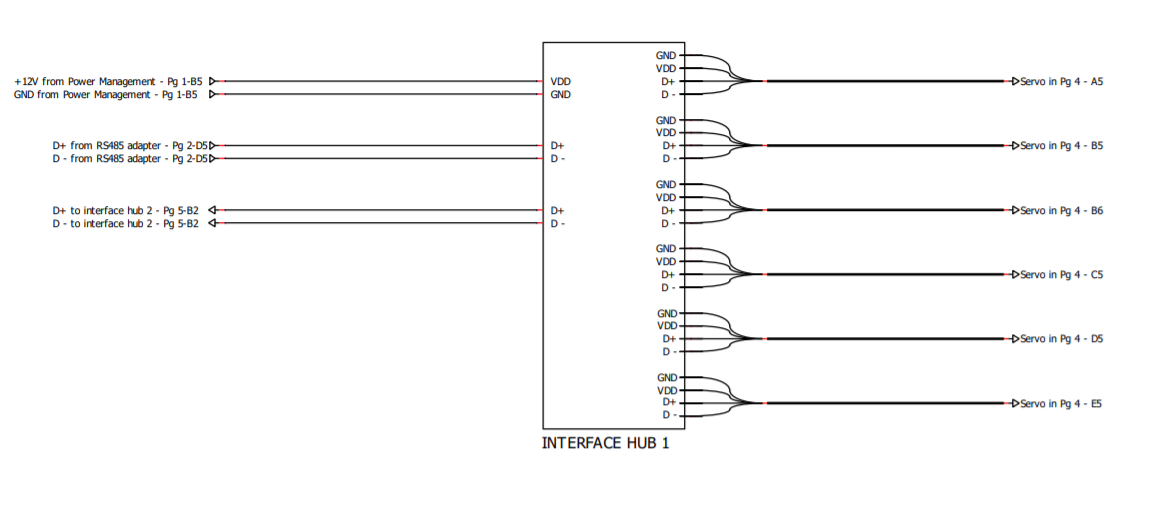
\includegraphics[width=0.4\textwidth]{esquema_hub.png}				
	\caption{Esquema das saídas do HUB.}		
	\label{img:hub1}									
\end{figure}

\begin{figure}[h!]												
	\centering												
	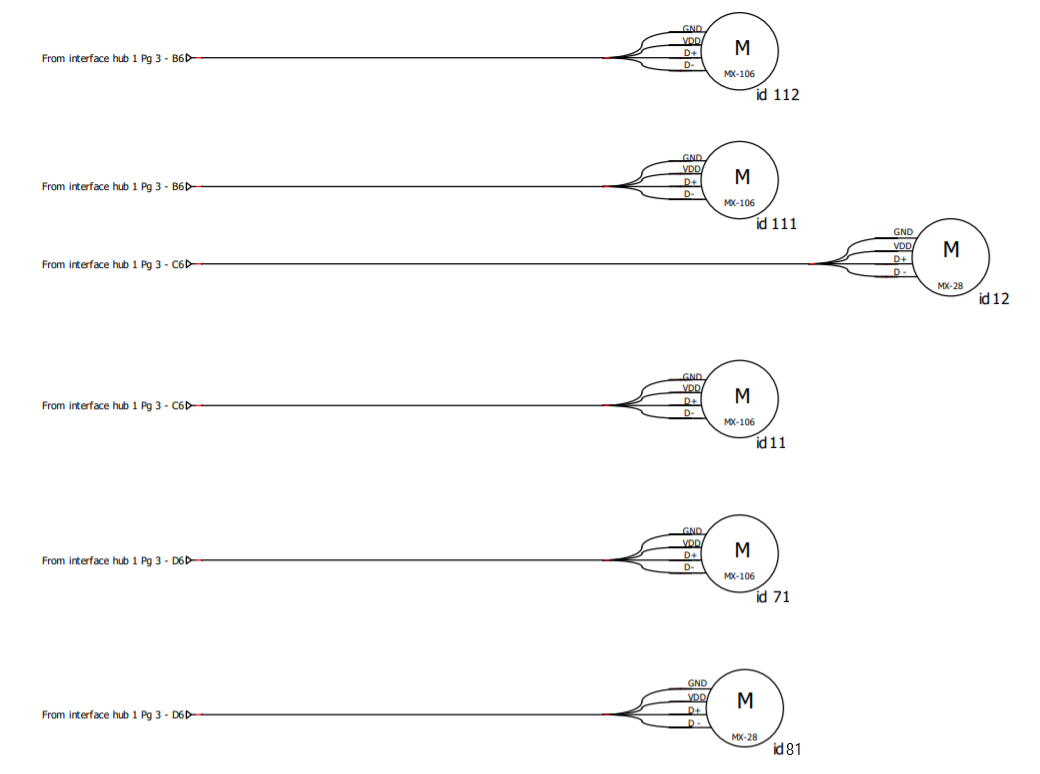
\includegraphics[width=0.4\textwidth]{esquema_hub2.PNG}				
	\caption{Esquema das conexões do HUB para os motores.}		
	\label{img:hub2}									
\end{figure}

\subsection{Esquemas eletrônicos}
\label{ssec:esqe}
Nas unidades de tração do robô, os hubs contam com um conector de alimentação, um para a entrada de dados e 6 de saída para os motores.
IMAGEM
\begin{figure}[h!]												
	\centering												
	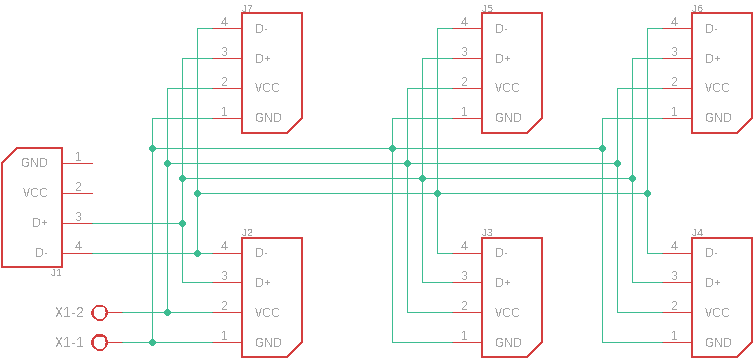
\includegraphics[width=0.3\textwidth]{hub_arm_SCHEMATIC.png}				
	\caption{Esquema HUB2.}		
	\label{img:hub2}									
\end{figure}

\begin{figure}[h!]												
	\centering												
	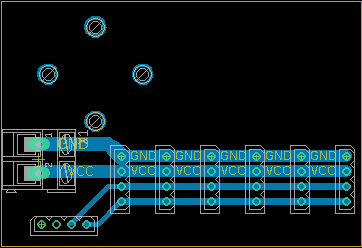
\includegraphics[width=0.3\textwidth]{hub_arm_BOARD.png}				
	\caption{Esquema HUB2.}		
	\label{img:hub2}									
\end{figure}

Já na unidade central, o hub além de conectar os seis motores ali presentes, também é responsável pela conexão dos hubs das unidades de tração e do conversor rs485 que está ligado à \textit{NUC}.
\begin{figure}[h!]												
	\centering												
	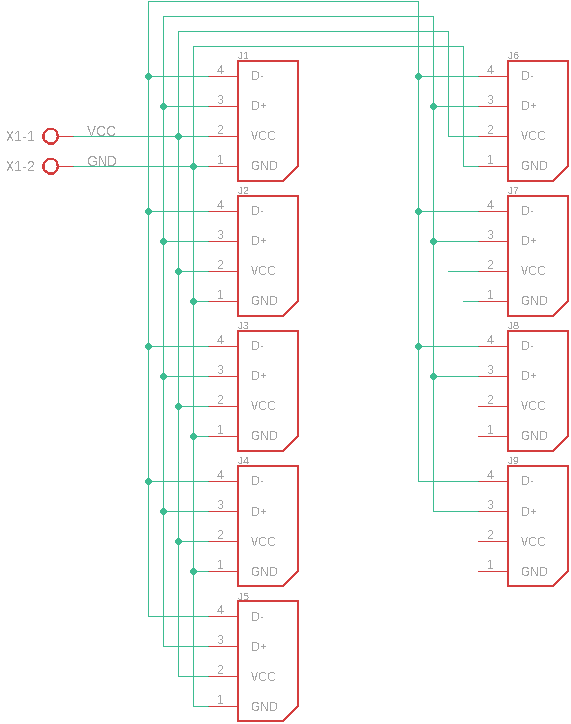
\includegraphics[width=0.3\textwidth]{hub_central_SCHEMATIC.png}				
	\caption{Esquema HUB2.}		
	\label{img:hub2}									
\end{figure}

\begin{figure}[h!]												
	\centering												
	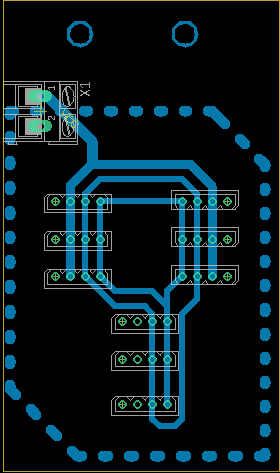
\includegraphics[width=0.3\textwidth]{hub_central_BOARD.png}				
	\caption{Esquema HUB2.}		
	\label{img:hub2}									
\end{figure}

%--------- NEW SECTION ----------------------
\section{Especificação das funcionalidades}
\label{sec:espf}


\subsection{Fluxo das informações}
\label{ssec:fluxo}

Diante da arquitetura apresentada anteriormente e focando nos objetivos traçados no Capítulo \ref{chap:introd}, o sistema robótico foi dimensionado para onze funcionalidades distintas:

\begin{enumerate}%[itemsep=1pt]
	%\setlength\itemsep{1em}
	\item sistema de verificação da integridade
	\item gerenciamento de energia
	\item aquisição
	\item localização
	\item planejamento de movimento
	\item atuação
	\item detecção
	\item classificação
	\item interface do usuário
	\item autonomia
	\item simulação
\end{enumerate}

A Figura \ref{img:elirfluxo} apresenta o fluxo de informações entre as funcionalidades. Este fluxo deve ser compreendido para que seja estabelecida as relações entre as funcionalidades e o entendimento entre elas, essa compreensão impactará na melhor elaboração da árvore de falhas do sistema e proporcionará um sistema mais confiável.

%---------------picture------------------------------------
\begin{figure} [h!]	
	\caption{Fluxo de informações do sistema.}
	\label{img:elirfluxo}											 
	\centering													 
	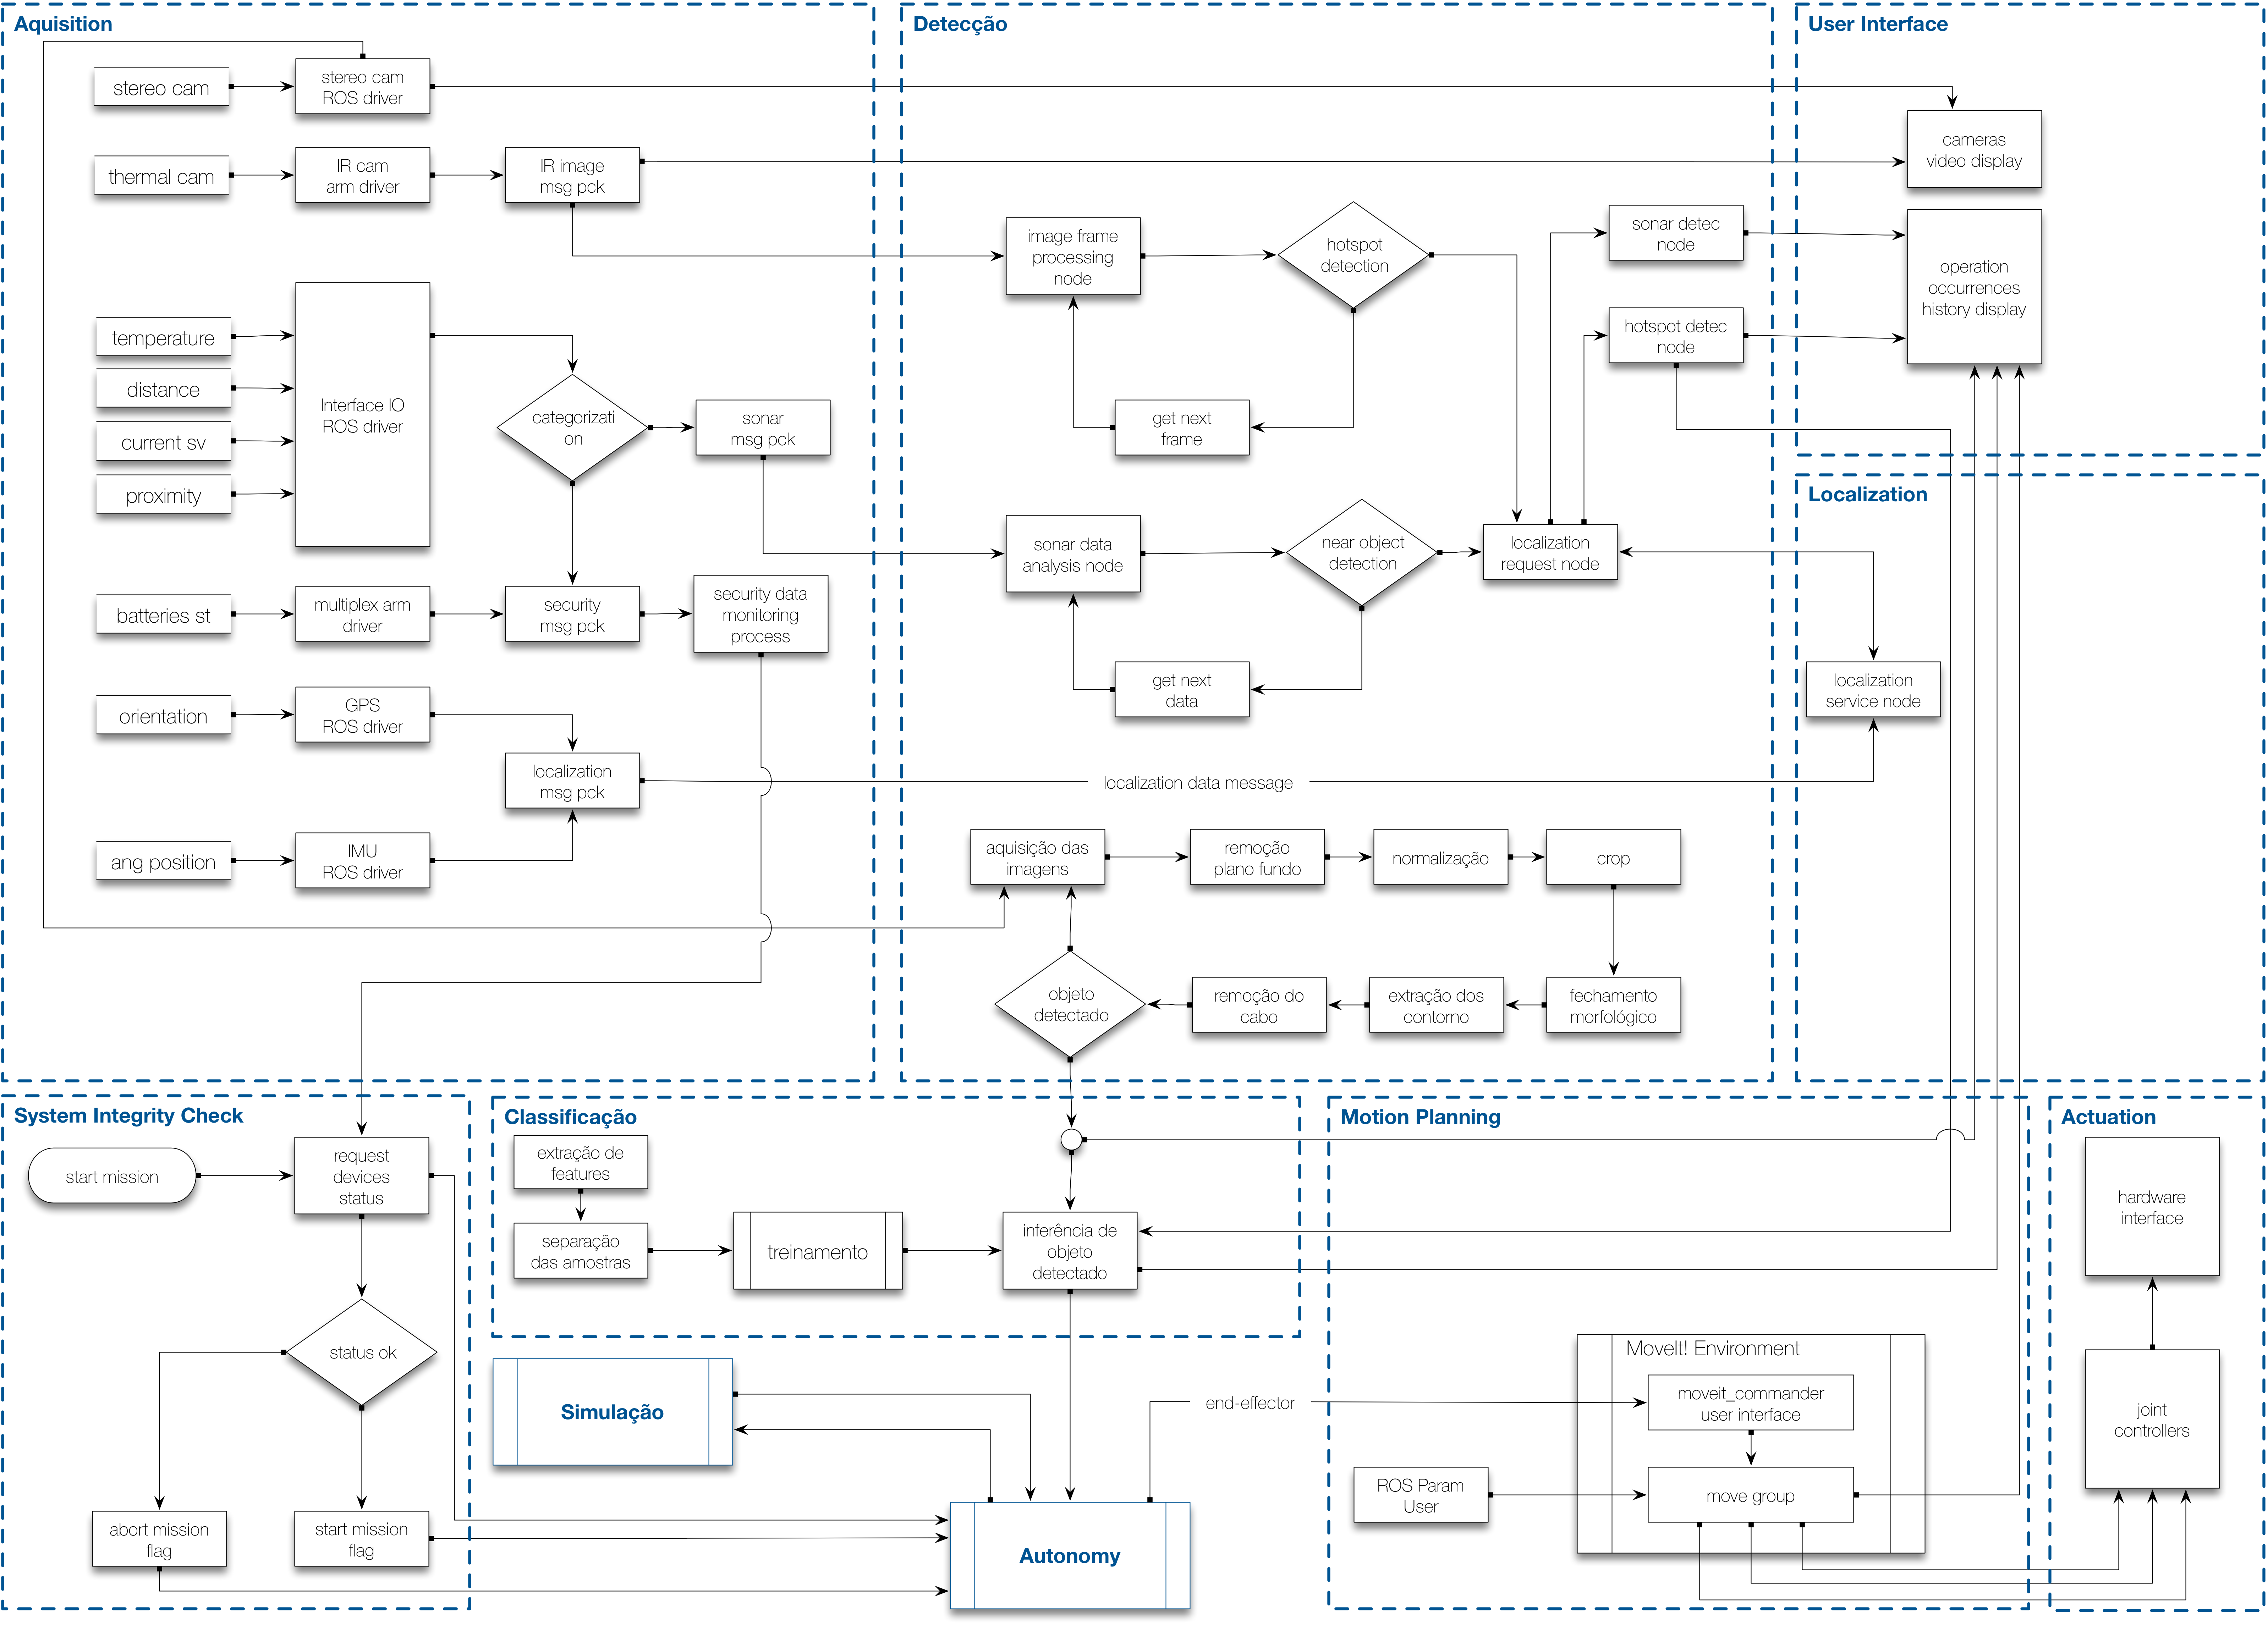
\includegraphics[width=1.0\textwidth]{Figures/flxinfofunctionalities}
	%\fautor			 											 
\end{figure}													 
%----------------------------------------------------------

Nas seções seguintes são apresentados em maiores detalhes sobre cada uma das funcionalidades do sistema robótico. Para que fosse melhor compreendido, o desenvolvimento destas funcionalidades foram agrupadas em cinco áreas: movimentação, percepção, interface do usuário, autonomia e simulação. As duas áreas iniciais foram subdivididas em planejamento de movimento, sistema de verificação de integridade, atuação e gerenciamento de energia para a primeira área de nome \textbf{movimentação}, que tem como principal objetivo garantir a execução da missão e transposição de obstáculos. Para a segunda área, nominada por percepção, a subdivisão ficou da seguinte forma: aquisição, detecção, classificação e localização, que como o significado do próprio nome apresenta como objetivo principal a percepção do robô diante do ambiente inserido.

%\subsection{Fluxo das informações}
%\label{ssec:fluxo}



\subsection{Motion Planning}
\label{ssec:motion}
%\subsubsection{Definição da funcionalidade}
A funcionalidade de \textit{Motion Planning} é responsável por realizar o planejamento da trajetória do Robô, utilizando o software \textit{MoveIt!} que realiza o cálculo da cinemática inversa para encontrar a melhor forma de ultrapassar os obstáculos.
\subsubsection{Dependências}
O software \textit{MoveIT!} pode utilizar o modelo matemático da cinemática inversa do robô ou um arquivo do tipo \textit{URDF}.
O nome \textit{URDF} é uma sigla para \textit{Unified Robot Description Format}, esse arquivo é uma especificação em \verb|XML| utilizada para descrever robôs. Modelos em \textit{URDF} apresentam uma simplicidade na descrição do robô, e para o caso do Robô \textit{Elir}, utilizar o modelo \textit{URDF} possibilitará uma aproximação fiel ao modelo real do robô, assim para o cálculo da cinemática inversa será utilizado o seu modelo \textit{URDF} e não o seu modelo matemático.

\subsubsection{Premissas Necessárias}
Para o correto funcionamento dessa funcionalidade as seguintes premissas são necessárias:
\begin{itemize}
	\item A configuração dos limites de giro das juntas do robô estarão compatíveis com os comandos enviados
	\item O modelo \textit{URDF} do robô estará adequado com o modelo físico
	\item O pacote gerado pelo \textit{MoveIt! Setup Assistant} estará configurado adequadamente
\end{itemize}
\subsubsection{Descrição da Funcionalidade}
A movimentação do robô na linha acontecerá por movimentos de translação e transposição de obstáculos. A translação na linha será feita por controladores de torque nas rodas do robô, enquanto a transposição do obstáculos utilizará o \textit{MoveIT!}.
Por meio da ferramenta \textit{MoveIt! Setup Assistant}, se utiliza o modelo do robô para criar um pacote do \textit{ROS} com os principais arquivos pelo \textit{MoveIT!}. 
A configuração correta do \textit{MoveIT!} possibilita que se utilizem as funções da sua biblioteca para o cálculo da trajetória, levando em consideração também obstáculos no caminho.

O \textit{MoveIT!} fornece uma \textit{user interface} que recebe o end-effector,a nomenclatura atribuída ao node feito em python que recebe o \textit{end-effector} é \verb|moveit_commander|. O  \textit{node} responsável por fazer a integração da user interface com os parâmetros recebidos pelo \textit{ROS Parameter Server} com o \textit{end-effector} para fazer os cálculos é denominado \verb|move_group|. O \textit{node} \verb|move_group| também pode receber parâmetros como leituras dos sensores do robô e nuvens de pontos.

\begin{figure}[!h]
	\centering
	\includegraphics[width=0.8\textwidth]{motion_plan_func.png}
	\caption{Fluxograma de funcionamento da funcionalidade de Motion Planning}
	\label{fig:flux_motion}
	\source{Própria}
\end{figure}

\subsubsection{Saídas}
Por meio da compatibilização do \textit{MoveIt!} com o \textit{ROS}, a saída dessa funcionalidade são os comandos de velocidade, esforço e posição para cada junta do robô.

\subsection{Actuation }
\label{ssec:actu}
\subsubsection{Definição da funcionalidade}
A funcionalidade de Actuation tem como objetivo mover a estrutura física do robô, possibilitando o controle dos movimentos das juntas, garras e unidades de tração.
\subsubsection{Dependências}
Essa funcionalidade depende das funcionalidades de \textit{Power Management} e \textit{Motion Planning}. O \textit{Power Management} será responsável por fazer alimentação dos motores, possibilitando controlar a corrente máxima fornecida para cada grupo.
A dependência em relação à funcionalidade de \textit{Motion Planning} está atrelada principalmente com o software \textit{MoveIt!}, que ao receber um \textit{end-effector},realiza o cálculo de trajetória e envia os comandos de velocidade, esforço e posição para os controladores das juntas, garras e unidades de tração.

\subsubsection{Premissas Necessárias}
Para o correto funcionamento desse módulo, devem ser consideradas as seguintes premissas:
\begin{itemize}
	\item Os motores devem estar configurados de acordo com o padrão de ID determinado pela equipe, fazendo parte da mesma malha de controle;
	\item Os controladores das juntas,garras e unidades devem estar configurados de acordo com os comandos que serão recebidos pelo\textit{ MoveIt!};
	\item Os 3 grupos de motores estarão em malhas de alimentação de 12V individuais.
\end{itemize}
\subsubsection{Descrição da Funcionalidade}
O \textit{ROS} disponibiliza uma série de drivers para compatibilização dos motores dynamixel, possibilitando a criação de controladores específicos no seu ambiente. Serão criados os controladores referentes as juntas e unidades de tração do robô.Os controladores receberão comandos de \textit{velocity} e \textit{position} do \textit{MoveIt!} junto com os comandos para movimentar o robô na linha.
Após os comandos serem recebidos pelos controladores, eles serão enviados para o \textit{hardware} do robô, de acordo do padrão de comunicação dos motores, por meio de comunicação serial. 
\begin{figure}[h]
	\centering
	\includegraphics[width=0.6\textwidth]{actuation_depen.png}
	\caption{Fluxograma da funcionalidade Actuation}
	\label{fig:depen_actuation}
	\source{Própria}
\end{figure}
\subsubsection{Saídas}
A saída desta funcionalidade é o movimento da estrutura física do robô, que estará de acordo com o planejamento de trajetória do \textit{MoveIt!} e com as instruções para operação na linha

\subsection{Power Management}
\label{ssec:power}
\subsubsection{Definição da funcionalidade}

A funcionalidade de \textit{Power Management} é responsável pelo gerenciamento de alimentação elétrica dos componentes elétricos e eletrônicos do robô, através da integração das funcionalidades de seu firmware no ambiente \textit{ROS}.
\subsubsection{Dependências}
Essa funcionalidade depende da comunicação serial por meio da biblioteca \verb|rosserial| para compatibilização e integração das funcionalidades de firmware no ambiente \textit{ROS}. Operacionalização e customização do firmware embarcado no hardware de acordo com as necessidades do projeto e da alimentação fornecida pela placa multiplexadora, por meio de baterias Li-Ion NH2054 14.4 volts.

\subsubsection{Premissas Necessárias}
Para o correto funcionamento desse módulo de \textit{Power Management}, devem ser consideradas as seguintes premissas:
\begin{itemize}
	\item A placa multiplexadora estará conectada diretamente ao módulo de \textit{Power Management} 
	\item Todos os dispositivos estarão conectados nas suas respectivas entradas
	\item A placa deverá ser alimentada por 2 baterias de 14.4 Volts e 3 Amperes, totalizando um fornecimento de até 6 Amperes
	\item A placa estará conectada diretamente na NUC, por meio de uma USB	
	
\end{itemize}
\begin{figure}[h]
	\centering
	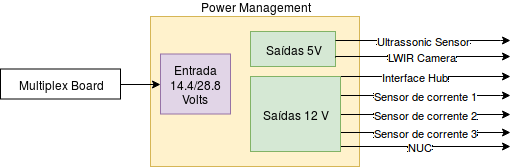
\includegraphics[width=1\textwidth]{power_management_hardware.png}
	\caption{Fluxograma de funcionamento da funcionalidade de Power Management}
	\label{fig:power_management_hardware}
	\source{Própria}
\end{figure}
\subsubsection{Descrição da Funcionalidade}
A funcionalidade \textit{Power Management} é responsável  fornece diversos recursos em sua totalidade. O hardware utilizado (placa Zord) possui um sensor de corrente e tensão para cada porta de saída, permitindo o monitoramento individual de cada uma das portas. O microcontrolador utilizado Atmega32U4 possui um firmware embarcado onde toda a compatibilização com o ambiente \textit{ROS} é realizada, o que torna essencial o uso do pacote rosserial para o seu funcionamento. O firmware é responsável pela ativação dos relés digitais em caso de surtos de corrente para proteção dos dispositivos elétricos. 
Os limites nos valores de corrente funcionam justamente para que o hardware interrompa a alimentação em um possível caso de surto de corrente. Todos os aspectos importantes para o funcionamento do sistema de gerenciamento de energia pode ser configurado tanto via \textit{ROS}, por meio das configurações dos serviços, ou por meio do firmware, modificando os parâmetros do tempo de duração dos picos de corrente. Os principais serviços e tópicos criados pela funcionalidade Power Management no \textit{ROS} são:
\begin{itemize}
	\item \textit{Tópicos}
	\begin{itemize}
		\item \textit{PowerOutput}
		Este tópico disponibiliza os valores de tensão e corrente de todas as portas da placa em tempo real.
		\item \textit{TakeStatus}
		Disponibiliza o estado de cada porta da placa, informando os eventos ocorridos e a porcentagem de corrente demandada durante a ocorrência do evento.
	\end{itemize} 
	\item \textit{Serviços} 
	\begin{itemize}
	\item \textit{GetCurrentLimitCommand}
	Este comando retorna o valor de corrente máxima de saída configurado para a porta escolhida
	\item \textit{SetCurrentLimitCommand}
	Este comando realiza a configuração do valor máximo de corrente de saída em uma determinada porta
	\item \textit{PowerOnOffCommand}
	Este comando realiza a ação de ativação ou desligamento de uma determinada porta.
	\end{itemize}
\end{itemize}
A placa de Gerenciamento de energia irá receber a carga das baterias pela placa multiplexadora e irá realiza o controle de alimentação dos seguintes componentes:
\begin{itemize}
	\item Grupos de servo motores
	\item Grupo de sensores de corrente
	\item NUC
	\item Interface HUB
	\item Câmera LWIR
	\item Sensor ultrassônico
	\item Phidgets
	\item STM Nucleo
	\item Módulo GPS
\end{itemize}

\subsubsection{Saídas}
A funcionalidade irá disponibilizar a energia para o robô e as seguintes estruturas no ambiente \textit{ROS}:
\begin{itemize}
	\item Tópicos com informações de tensão e corrente nas portas
	\item Tópico para aviso de sobre-corrente
	\item Tópico para informar disponibilidade da placa
	\item Serviços para ler e configurar limite de corrente das portas
	\item Serviço para ligar ou desligar energia em uma porta	
\end{itemize}

\subsection{System Integrity Check}
\label{ssec:check}

\subsubsection{Definição da funcionalidade}
É a funcionalidade responsável por checar a integridade do sistema antes do início da missão, verificando os subsistemas e suas variáveis.

\subsubsection{Dependências}
A funcionalidade receberá informações dos seguintes componentes
\begin{itemize}
	\item Sensor de Temperatura
	\item Servomotores
	\item Câmera IR
	\item Câmera Stéreo
	\item IMU
	\item Sensor de Proximidade
	\item Placa de Power Management
	\item Sonar 
	\item Baterias
\end{itemize}

Todas as informações serão enviadas por meio do ambiente \textit{ROS}, na forma de \textit{Services} ou \textit{Publishers}.

\subsubsection{Premissas Necessárias}
As premissas necessárias para o funcionamento dessa funcionalidade são:
\begin{itemize}
	\item Os subsistemas do robô irão disponibilizar o seu status no ambiente \textit{ROS} por meio de tópicos ou serviços
	\item A checagem fará parte do planejamento de missão
\end{itemize}

\subsubsection{Descrição da Funcionalidade}
A checagem da integridade do sistema é uma funcionalidade essencial para garantir o sucesso da missão e preservar a integridade do robô. O \textit{ROS} facilita essa comunicação entre os subsistemas, possibilitando que seja criada uma rotina de checagem antes de cada missão.

Será disponibilizado no sistema uma rotina para iniciar a missão. Ao receber o comando para início de missão, os sistemas serão checados sequencialmente, utilizando estrutura de \textit{Services} e \textit{Publishers} do \textit{ROS}. Caso algum sistema apresente falha, a missão não se iniciará e o erro será mostrado no \textit{terminal} e registrado no arquivo de \verb|log|. Se todos os sistemas estiverem em funcionamento, se iniciará a missão. O fluxograma da funcionalidade está ilustrado na figura \ref{fig:sys_check_flux}.	
\begin{figure}[h]
	\centering
	\includegraphics[width=0.6\textwidth]{sys_check_flux.png}
	\caption{Fluxograma da rotina para checagem do sistema}
	\label{fig:sys_check_flux}
	\source{Própria}
\end{figure} 


\subsubsection{Saídas}
No início da rotina de inspeção, a funcionalidade será responsável por enviar o sinal inicia a missão. Caso todos os sistemas checados estejam funcionando, a inspeção ocorrerá normalmente, se algum sistema apresentar defeitos, o defeito será mostrado no \textit{terminal}, registrado em log e a missão será abortada.


%--------- NEW SECTION ----------------------
\section{Simulação do sistema}
\label{sec:sim}
A simulação de sistemas robóticos consistem em um dos pilares para o desenvolvimento de projetos. Com a simulação é possível testar aplicações sem a necessidade de adquirir componentes, os membros da equipe de projeto conseguem trabalhar de forma simultânea no robô enquanto o protótipo físico fica reservado para testes específicos.

O \textit{ROS} oferece ferramentas de visualização já integradas no seu sistema, o RVIz, que possibilita o usuário visualizar os modelos do robô e também administrar plugins, como de mapeamento e planejamento de movimento, que é o caso do \textit{MoveIt!}.



Para a simulação do robô no ambiente aberto, é utilizado  o software \textit{Gazebo}. A integração entre \textit{ROS} e \textit{Gazebo} consegue fazer com que o modelo \textit{URDF}, por mais que não seja o nativo do \textit{Gazebo}, seja aceito na simulação. Parâmetros do mundo podem ser ajustados e a integração de plugins como câmeras e sensores faz com que a simulação consiga ser utilizada em diferentes estudos. Algoritmos de imagem podem ser testados com os plugins de câmera já implementados, proporcionando um auxílio para demonstrar conceitos e teorias de funcionamentos

A simulação fornecida possui os controladores de juntas já implementados, fazendo com que testes de códigos de movimentação e testes de controles já pudessem ser previamente testados, poupando riscos de dano ao protótipo e possibilitando trabalho simultâneo.

\begin{figure}[h!]												
	\centering												
	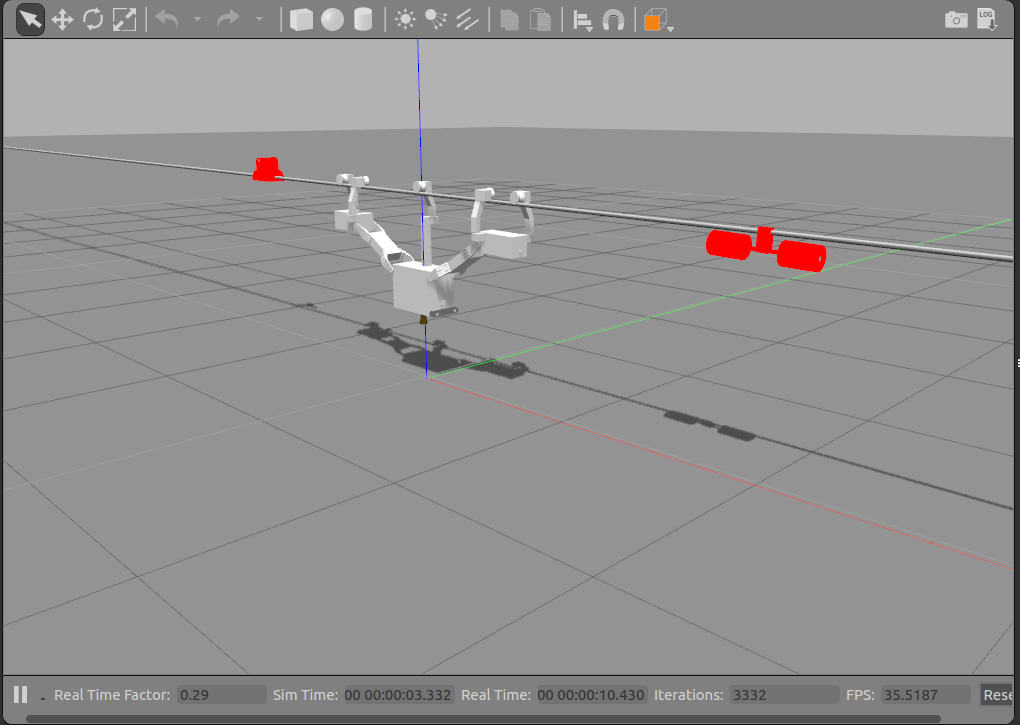
\includegraphics[width=0.6\textwidth]{elir_no_gazebo.png}				
	\caption{Simulação do \textit{ELIR} no \textit{Gazebo}.}		
	\label{img:gazebo1}									
\end{figure}


    \chapter{Desenvolvimento e testes}
\label{chap:desen_test}
Durante o desenvolvimento do projeto, foram feitos diversos estudos relacionados com o âmbito da robótica. A diversidade de ferramentas existentes faz com que o pesquisador tenha diversos formas de alcançar um resultado final e por se tratarem de conhecimentos específicos, cada ferramenta exige complexidade e dedicação para que seu domínio seja efetivo e resultados satisfatórios sejam alcançados.

A constante pesquisa e trabalho com as mesmas ferramentas definidas no início do processo metodológico possibilitou a realização de diversos testes, buscando validar as decisões tomadas, assim como aumentar o domínio das ferramentas e descobrir a melhor forma de utilizar todo seu potencial.

Os dispositivos eletrônicos oferecem muita informação sobre o seu funcionamento, porém, é necessário conhecer o seu comportamento na prática, já que esses dispositivos serão expostos a situações específicas do projeto, além de que, por estarem funcionando em conjunto com diversos subsistemas, é importante conhecer o seu comportamento quando como organismo de um sistema maior.

Com o decorrer do fluxo metodológico diversos tipos de resultados foram alcançados, seja conhecimento específico de uma ferramenta, validação da sua funcionalidade para um sistema específico ou seu comportamento como um organismo.  O conceito do sistema é algo fundamental e o mesmo foi um fruto dessa metodologia, onde as suas funcionalidades desempenham um importante papel para se conhecer a idéia.

%--------- NEW SECTION ----------------------
\section{Análise das Funcionalides}
\label{sec:analise_func}
O desenvolvimento do conceito do sistema resultou nas funcionalidades, que por sua vez representam o fluxo das informações. A forma de estabelecer esse fluxo foi idealizando a operação do robô, buscando se determinar as atividades à serem desenvolvidas.

A inspeção de linha, exemplificada como o ato de caminhar na linha e ultrapassar um obstáculo, foi denominada missão. Assim, cada vez que o robô inicia esse processo, é iniciada uma missão.

De forma a garantir a execução da missão de forma efetiva, utilizou-se os requisitos fornecidos para o cliente e o QFD 1 aliado ao estudo das ferramentas para determinar os subsistemas presentes no robô, produzindo assim uma versão do QFD 2 aliada com a definição das funcionalidades para o sistema robótico, já que ambas aconteceram em paralelo e são complementares, o QFD 2 está mostrado na figura \ref{fig:qfd2} , estando disponível no anexo X.

\begin{figure}[H]
	\centering
	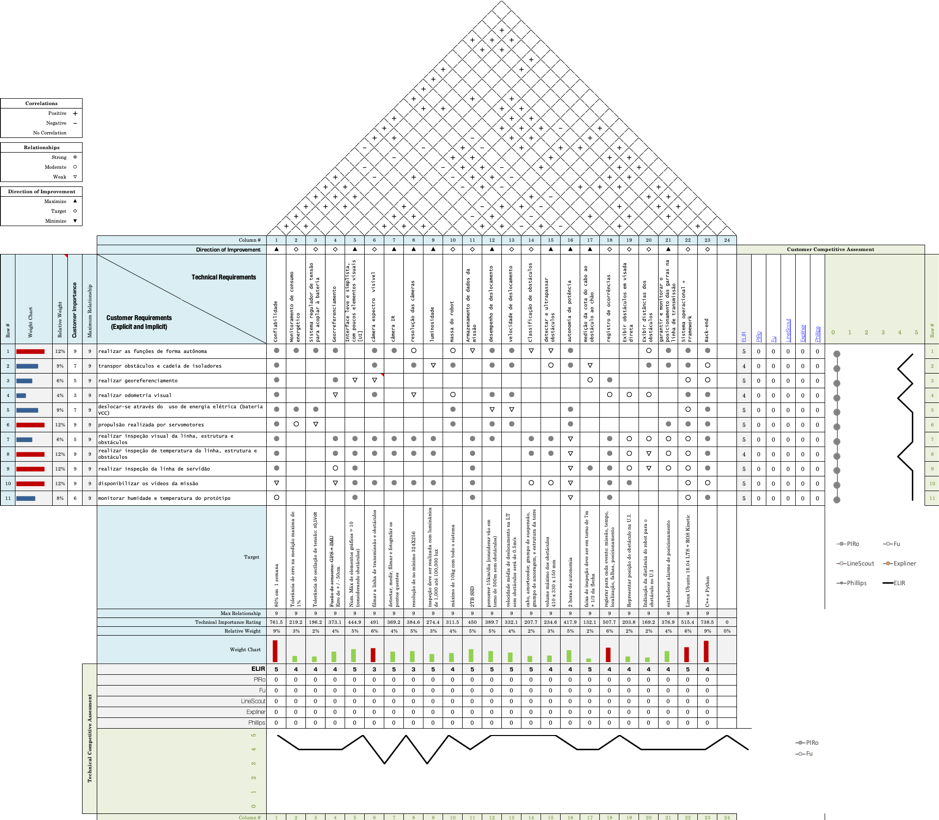
\includegraphics[scale=1]{Figures/qfdelir-2.png}
	\caption{QFD 2}
	\label{fig:qfd2}
\end{figure}

Com uma idealização do fluxo do sistema e suas funcionalidades, foi elaborada uma arquitetura geral do sistema de movimentação, mostrada na figura \ref{fig:arq_geral} e disponível no anexo X.  Antes do início da missão, é necessário que o sistema esteja apto a tal, assim foi definida uma funcionalidade para verificação da integridade do sistema, que requisita os status dos dispositivos antes de realizar a missão por meio de uma checagem, e com o sucesso na checagem, fornece o comando para o início.

\begin{figure}[H]
	\centering
	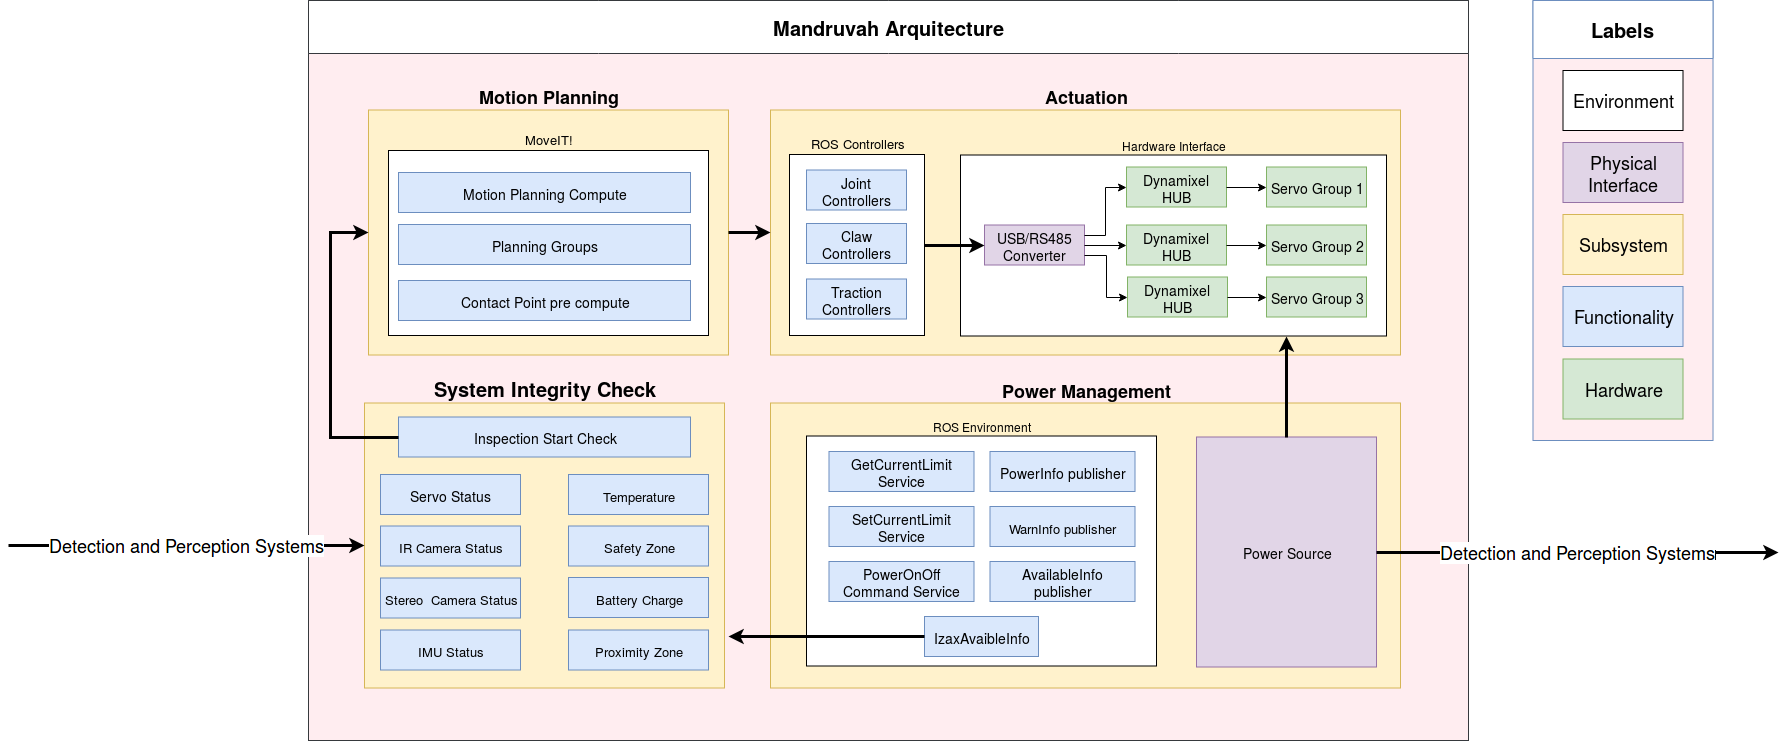
\includegraphics[scale=0.25]{Figures/Arquitetura.png}
	\caption{Arquitetura geral do sistema de movimentação}
	\label{fig:arq_geral}
\end{figure}
eterminou-se que a funcionalidade responsável pelo Planejamento de Movimento, realizasse o cálculo do plano de movimento junto com a administração dos grupos de controle e o cálculo de pontos de contato no robô. Onde essas informações sobre o plano de movimento do robô seriam transferidas para a funcionalidade de atuação do robô, que é responsável por receber esses comandos nas estruturas padrão do \textit{ROS} e realizar o movimento físico do robô.

A movimentação exige muita energia do robô e aliado devido a necessidade do controle da potência disponível, foi idealizada a funcionalidade de Gerenciamento de energia, responsável por disponibilizar as informações de energia no ambiente \textit{ROS} e fornecer a energia para o sistema de alimentação.

\subsection{Atuação}\label{sec:actuation}
Com a arquitetura geral do sistema de movimentação e o fluxo de comunicação, foi possível estabelecer as propriedades específicas da funcionalidade de atuação, onde buscou-se definir suas dependências, saídas e seu funcionamento.

Foi feito um fluxograma para representar a funcionalidade, onde estão ilustrados todos seus parâmetros, como mostra a figura \ref{fig:flux_atu}.

\begin{figure}[H]
	\centering
	\includegraphics[scale=0.5]{Figures/actuation_depen.png}
	\caption{Fluxograma da funcionalidade de Atuação}
	\label{fig:flux_atu}
\end{figure}

Os comandos relativos a posição, esforço e velocidade para as juntas vêm da funcionalidade de planejamento de movimento, onde a atuação recebe esses comandos, transferindo os mesmos para os controladores do ambiente \textit{ROS} que se comunicam com a interface de \textit{hardware} que envia o comando para os motores realizarem o movimento.
\subsection{Planejamento de Movimento}\label{sec:plan_mov}
A forma que o robô vai realizar seus movimentos é determinado pela funcionalidade de Planejamento de Movimento. Que por sua vez tem a ferramenta \textit{MoveIt!} como importante componente para que a movimentação ocorra de forma efetiva, sendo assim, as unidades de \textit{software} da ferramenta que irão se comunicar com a funcionalidade explicitadas no fluxograma \ref{fig:fluxo_motion} estão incluídas no ambiente do \textit{MoveIt!}, recebendo o comando da posição desejada para o end-effector e enviando os comandos necessários para as juntas. 
	
\begin{figure}[H]
	\centering
	\includegraphics[scale=0.4]{Figures/motion_plan_func.png}
	\caption{Fluxograma da funcionalidade de Planejamento de Movimento}
	\label{fig:fluxo_motion}
\end{figure}

		
Apresenta uma dependência do sistema de autonomia do robô, que envia uma posição de referência o robô, o que culmina na necessidade da ultrapassagem de um obstáculo, já que, em operação, a ultrapassagem de obstáculos acontece diversas vezes. A rotina de ultrapassagem de obstáculo então envia para o \textit{software} o end-effector necessário para a ultrapassagem, e consequentemente são enviados os comandos contendo  a posição,esforço e velocidades das juntas para a funcionalidade de atuação.

\subsection{Gerenciamento de Energia}\label{sec:geren_ener} 
A necessidade de distribuir a energia elétrica proveniente de uma bateria entre os sistemas eletrônicos do robô, de maneira inteligente se mostrou uma parte fundamental do projeto. Para que isso fosse implementado, houve a necessidade de desenvolver uma funcionalidade responsável por monitorar os níveis de corrente e tensão fornecidos para cada um dos dispositivos eletrônicos do robô, permitindo a criação de um sistema de proteção contra surtos de corrente, com ajuste de limites para valores do fornecimento de corrente.

Após a análise e constatação da necessidade da implementação desta funcionalidade, foram feitas as definições de quais seriam suas entradas, saídas e suas dependências.

A funcionalidade de gerenciamento de energia depende essencialmente da placa multiplexadora, a qual é responsável por alimentar o \textit{hardware} de \textit{Power Management} com a energia proveniente das baterias, e de que todos os seus drivers e funções estejam instaladas no ambiente \textit{ROS}, para que seja possível utilizar as suas ferramentas.

O sistema de \textit{power management} cria no ambiente \textit{ROS}, estruturas de \textit{software} responsáveis por permitir o monitoramento das portas de alimentação (informando valores de tensão e corrente), bem como a configuração dos limites do fornecimento de corrente e a desativação ou acionamento dos relés digitais de cada uma das portas.

O gerenciamento de energia monitora os valores de corrente fornecidos nas portas, e verifica  ocorrência de possíveis surtos, verificando o valor do pico e o tempo de duração. Caso seja detectado um surto de corrente, o fornecimento da porta é desativado, protegendo assim o sistema como um todo.

Uma vez que o estudo do \textit{hardware} e das suas funções no ambientes \textit{ROS} estavam completos, foram iniciados os primeiros testes com partes isoladas do robô para verificar o comportamento do \textit{hardware} e se o seu funcionamento estava de acordo com o esperado, para atender os requisitos da funcionalidade de maneira satisfatória, para assim ser integrado ao sistema.


\subsection{Checagem da Integridade do Sistema}\label{sec:check_sis}
Todas os sistemas do robô devem operar de maneira correta, para garantir o sucesso na execução da missão, e a partir desta observação, foi concebida a funcionalidade de checagem de integridade do sistema. Sua principal função é garantir que todas os sistemas do robô estejam sem apresentar falhas antes do início da missão. Uma vez que a checagem é realizada, o robô pode iniciar a sua missão.

Esta funcionalidade se mostra importante pelo fato de que a checagem prévia, reduz significantemente os riscos e prejuízos atrelados a uma má execução da missão, como componentes danificados e perda na eficiência durante toda a missão. Todos os sistemas que irão participar da missão, devem estar atrelados ao sistema por meio do ambiente \textit{ROS}, onde cada um irá informar o seu estado para a funcionalidade. O fluxograma \ref{fig:fluxo_check} foi desenvolvido para ilustrar o funcionamento da rotina de checagem integridade do sistema.

\begin{figure}[H]
	\centering
	\includegraphics[scale=0.4]{Figures/sys_check_flux.png}
	\caption{Fluxograma da funcionalidade de Checagem da Integridade do Sistema}
	\label{fig:fluxo_motion}
\end{figure}
Uma vez que esta funcionalidade foi concebida, toda as outras integrantes do sistema, deveriam se integrar ao sistema de integridade para garantir que a missão pudesse ser iniciada sem erros graves.

\section{Estudo da Movimentação}\label{sec:estud_mov}
Para o desenvolvimento das ferramentas para ultrapassagem de obstáculos, foi necessária a análise dos movimentos necessários para que fosse realizada a ultrapassagem de obstáculos. Os tipos de movimento a serem realizados influenciam nas ferramentas escolhidas para o controle e operação do robô, já que se busca a otimização do movimento e também redução do tempo gasto no desenvolvimento, de forma a garantir um resultado satisfatório.

Foi feita uma análise utilizando como referência o maior obstáculo, que foi o amortecedor, mostrado na figura \ref{fig:amortecedor} e levando em consideração a sua modelagem como um paralepipedo de dimensões 535mm. Constatou-se que seria necessário que para a ultrapassagem desse obstáculo, o robô necessitaria abrir um dos braços e se deslocar somente com a unidade de tração central e outro braço. Para isso seriam necessários movimentos para abrir e fechar as garras do robô, assim como um comando específico para afastar a unidade de tração da linha a distância necessária para a abertura da garra. Assim como o movimento que abre o braço o suficiente para que esse passe abaixo do obstáculo.

A ferramenta de visualização presente no ROS, possibilitou testar os limites de giros das juntas e visualizar como seriam as poses do robô sem a necessidade da simulação. O conhecimento relacionado à como a movimentação ia ocorrer possibilitou nortear o desenvolvimento.
\begin{figure}[H]
	\centering
	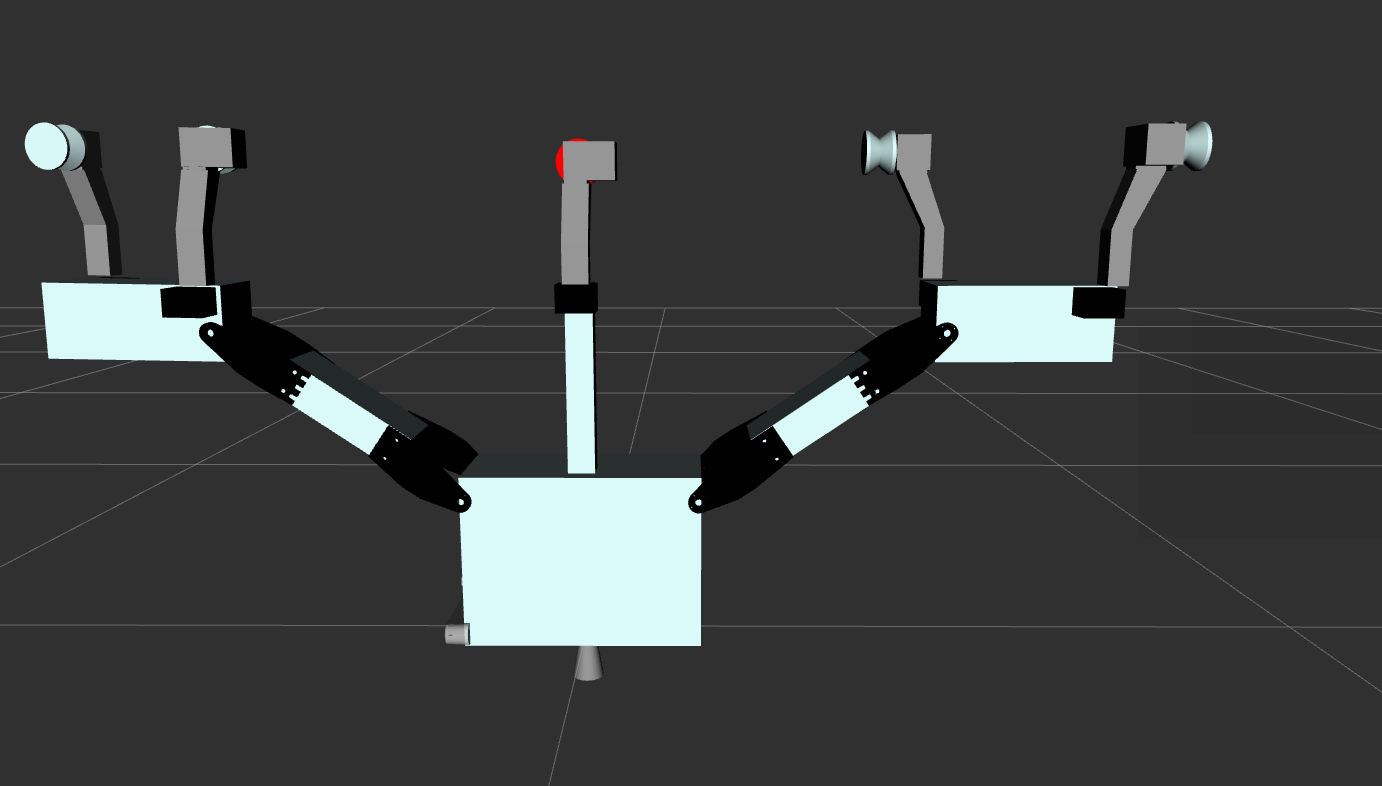
\includegraphics[scale=0.25]{Figures/rviz_garra_aberta.png}
	\caption{Robo \textit{ELIR} no visualizador do \textit{ROS} com garras abertas}
	\label{fig:elir_garras abertas}
\end{figure}
\section{Soluções Mecatrônicas para o sistema robótico}\label{sec:sol_sis}
Uma vez que os principais aspectos das funcionalidades estavam definidos, foi necessário realizar a implementação das soluções mecatrônicas no robô. Foram realizados estudos de dispositivos eletrônicos e das suas ferramentas de configuração, bem como programas e \textit{software}s que seriam necessários para a implementação das funcionalidades.

\subsection{Escolha a biblioteca de controladores no \textit{ROS}}\label{sec:contr_ros}
Para implementar as rotinas de controle e atuação dos motores Dynamixel, era necessário que houvesse algum meio de configurá-lo para operar de maneira desejada, podendo realizar a criação de juntas, e unidades de tração. Especificamente nos motores Dynamixel, isto é possível através da utilização de drivers.

Os drivers são estruturas de \textit{software} que permitem a compatibilização do dispositivo físico com uma interface computacional, habilitando as suas funções e configurações dentro de um ambiente de \textit{software}, permitindo que o dispositivo possa ser configurado e ter suas funções utilizada através de comandos provenientes de uma camada de \textit{software} superior.

A movimentação das juntas e eixos do robô se dá pelo uso de servomotores, e para que os mesmos sejam controlados pelo framework, que no caso é o \textit{ROS} - é necessário fazer uso de um driver.

Diante a variedade de bibliotecas para controlar os motores da dynamixel no ros disponíveis, foi necessário escolher qual será utilizada. Para escolha a biblioteca foram levados alguns parâmetros que influenciam para o fluxo de informações e funcionalidades do robô, assim como complexidade de código, disponibilidade de tutoriais, suporte pela comunidade, as ferramentas disponíveis, compatibilidade do firmware, etc.

Foram selecionadas 2 bibliotecas que são disponibilizadas pelo próprio framework \textit{ROS}, sendo elas: a  \textit{dynamixel\_drivers} e a \textit{dynamixel\_workbench}. A escolha pela \textit{dynamixel\_drivers} se deu pelo fato ser mais velha e por consequência mais materiais disponíveis para consulta, apesar a workbench possuir suporte para novas versões do dynamixel, essa possibilidade não teve muitos benefícios, já que o projeto foi utilizado para versões antigas de motores. 

\subsection{Solução para cinemática}\label{sec:sol_cine}
O cálculo da cinemática pode ser realizado de diferentes formas, já que o mesmo parte da modelagem do robô por meio de um conjunto de equações. Existem diferentes solucionadores para problemas de cinemática, que podem utilizar diferentes parâmetros de entrada.

No âmbito da robótica podem ser utilizados tanto os modelos matemáticos já elaborados pelos desenvolvedores, como também o modelo 3D do robô. Esse modelo 3D é definido geralmente por meio de arquivos do tipo \textit{URDF} , que utilizam uma escrita simples, definindo o robô a partir de seus links e juntas. Esse arquivo é o mesmo utilizado para colocar o modelo do robô na simulação, e também é a forma padrão utilizada pelo \textit{software} \textit{MoveIt!}.
Com o estudo do estado da arte fornecido, não era necessário encontrar o conjunto de equações que descrevem o robô, e com a simulação fornecida, também já era possível utilizar o modelo \textit{URDF}. Foi feita uma análise entre as possíveis soluções cinemáticas, buscando encontrar a que garantisse um maior sucesso e facilitasse o desenvolvimento. Levando em consideração a disponibilidade de códigos e tutoriais para serem tomados como base, assim como o uso em projetos semelhantes, a complexidade da aplicação e integração com as estruturas do \textit{ROS}.

Assim levantou-se 3 possível soluções para o cálculo da cinemática inversa, sendo elas: o uso do modelo matemático já existente proveniente do estudo do estado da arte, sendo realizada sua solução manualmente por meio de códigos de programação, o uso da ferramenta \textit{MoveIt!} utilizando o modelo \textit{URDF} proveniente da simulação, e o uso da ferramenta \textit{MoveIt!} compatibilizada com modelo matemático.

A uso do modelo matemático completo para o robô, realizando a  solução por meio de um código, se mostrou inviável, já que também seria necessário a integração com as estruturas de controle do \textit{ROS}, e mesmo a implementação desse modelo no \textit{MoveIt!} não se mostrou a melhor opção, devido a alta complexidade e a falta de projetos semelhantes para consulta, tal qual a inexistência de tutoriais voltadas para essa aplicação em específico. Assim sendo escolhido o uso da ferramenta \textit{MoveIt!} com o modelo \textit{URDF} proveniente da simulação, já que esse mesmo modelo já é estudado pela equipe, para seu uso na simulação e a aplicação padrão do \textit{MoveIt!} utiliza esse modelo.

Essa solução utiliza os dados sobre o modelo do robô contidos no modelo \textit{URDF} para realizar o cálculo da cinemática de forma analítica, gerando diversas trajetórias e encontrando a melhor possível, baseada nos parâmetros configurados pelo usuário.

\subsection{Gerenciamento de Energia}\label{sec:geren_ene}
A implementação da funcionalidade de gerenciamento de energia foi possível através da utilização de um \textit{hardware} de \textit{Power Management}, uma placa eletrônica, fornecida pelo cliente do projeto, iniciando assim a primeira etapa do desenvolvimento da funcionalidade de gerenciamento de energia, a qual se deu pelo estudo do \textit{hardware}, através da leitura de \textit{datasheets} e esquemas elétricos. 

A placa contém sete portas de alimentação gerenciadas por relés digitais sendo cinco delas de 12 Volts e duas de 5 Volts. Dentre as portas de 12 Volts, 4 possuem regulação de fornecimento de corrente, onde o controle do fornecimento é realizado por um microcontrolador Atmega32U4. Todas as portas possuem sensores de tensão e corrente individuais, facilitando e otimizando o processo de leitura dos . O \textit{firmware} embarcado na placa de \textit{Power Management} possui a principal de função de implementar os relés digitais, onde se realiza uma leitura dos valores de corrente que estão sendo demandados pelas portas. 

Para que a integração do \textit{hardware} de \textit{Power Management} fosse realizada ao projeto foi necessário validar o seu funcionamento , e se os valores de tensão fornecidos, estariam de acordo com o configurado. As medições lidas no multímetro e no \textit{software}, foram registradas e comparadas, verificando se os valores de erro eram muito altos. Como mostra a Tabela \ref{tab:med_pow} a seguir:

\begin{table}[H]
	\centering
	\caption{Medições de tensão para o \textit{hardware} de \textit{Power Management}}
	\label{tab:med_pow}
	\begin{tabular}{ccc}	
		\hline
		\multicolumn{1}{r}{Porta Lida}      & Tensão - Multímetro         & Tensão - \textit{Software}         \\ \hline
		Porta 1                                            & 12.03 Volts          & 12.043 Volts     \\ \hline
		Porta 2                                           & 12.01 Volts     & 12.037 Volts          \\ \hline
		Porta 3                                           & 12.01 Volts     & 12.038 Volts          \\ \hline
		Porta 4                                           & 12.01 Volts     & 12.037 Volts          \\ \hline
	\end{tabular}
\end{table}
Foi possível perceber uma pequena variação na leitura em \textit{software} para a leitura realizada pelo instrumento de medição, apesar disso, pelo fato do erro ser de uma ordem baixa para os níveis de operação do robô, considerou-se que esta variação não representaria risco para a operação, validando assim o funcionamento do \textit{hardware} da \textit{Power Management}.


\section{Simulação}\label{sec:simul_result}
A estrutura do sistema \textit{ROS} e suas ferramentas já compatibilizada faz com que a simulação do sistema impacte de forma efetiva e positiva durante o processo de desenvolvimento. O \textit{software} Gazebo é uma das ferramentas para simulação  de ambientes robóticos mais utilizadas atualmente, por apresentar integração nativa com o sistema \textit{ROS} e foi utilizada para o projeto.

Os arquivos para  simulação do robô foram fornecidos pelo cliente, e apresentam características semelhantes às esperadas no robô real, como o tipo dos controladores de juntas, que são o padrão do \textit{ROS}, sendo os mesmos utilizados para o robô real, e consistindo assim um parâmetro fundamental para a simulação do sistema de movimentação.

Por apresentar os mesmos tipos de controladores do robô real, foi possível utilizar a simulação para validar a compatibilização do controle da ferramenta \textit{MoveIt!} com os controladores presentes no robô. Essa alternativa possibilitou a compatibilização entre as funcionalidades sem a necessidade do protótipo do robô pronto funcional, economizando tempo do desenvolvimento, já que reduz dependência entre as fases do desenvolvimento.

\subsection{Simulação para a rotina de ultrapassagem}\label{sec:simu_ultr}
A automatização dos movimentos do sistema é necessária para que ocorra a ultrapassagem, sendo assim esse conjunto de movimentos denominado de rotina. As estruturas do \textit{ROS} possibilitam a criação de estruturas que quando acionadas realizam comandos específicos.

Por apresentar os mesmo controladores, e com o auxílio do estudo dos movimentos necessários para a ultrapassagem, foi possível desenvolver os códigos que enviam os comandos específicos para os controladores.


\section{Testes de Movimentação Física}\label{sec:test_mov}
Os testes de movimentação física buscam compreender e validar os movimentos realizados pelo robô, indo desde da análise individual das partes do robô como braços e unidade de tração, até sua movimentação em conjunto.

\subsection{Testes unitários}\label{sec:test_mov_uni}
Os primeiros testes foram feitos com a estrutura parcialmente montada, já que o objetivo do teste é validar o funcionamento dos controladores de junta do \textit{ROS}, que é a base para o desenvolvimento das funcionalidades de Actuation e Planejamento da Movimentação. Nestes testes, foram estabelecidos os limites de movimentação das juntas, com o intuito de preservar a integridade física dos componentes. As juntas dos braços do robô ELIR são compostas por dois servomotores Dynamixel MX-106R fabricados pela Robotis. 

No decorrer desses primeiros testes, ocorreram falhas nos motores por excesso de carga em um deles, o que era configurado como mestre. Verificou-se que isso poderia ser contornado com o uso do cabo de sincronização ligando os dois motores de cada junta, já que os motores se comunicariam diretamente entre si para balancear a divisão da carga sobre a junta. Também foi o momento de analisar como se comportavam os servomotores utilizados nas juntas, sob influência do cabo de sincronização.
\begin{table}[H]
	\centering
	\caption{Sentido de giro dos motores (Cabo de sincronização direto)}
	\begin{tabular}{ccc}	
			\hline
		\multicolumn{1}{r}{Valor pulicado na junta:}      & Positivo         & Negativo         \\ \hline
		Mestre                                            & Horário          & Anti-horário     \\ \hline
		Escravo                                           & Anti-horário     & Horário          \\ \hline
	\end{tabular}
\end{table}

\begin{table}[H]
	\centering
	\caption{Sentido de giro dos motores (Cabo de sincronização cruzado)}
	\begin{tabular}{ccc}
		\hline
		
		\multicolumn{1}{r}{Valor pulicado na junta:}       & Positivo       & Negativo           \\ \hline
		Mestre                                             & Horário        & Anti-horário       \\ \hline
		Escravo                                            & Horário        & Anti-horário       \\ \hline
	\end{tabular}
\end{table}

Levando em conta que, para realizar o movimento corretamente, os motores tem que se movimentar em sentidos opostos, já que estão fisicamente invertidos, caso seja utilizado o cabo de sincronização cruzado, os motores escravos devem ser configurados com o modo de giro reverso.

\subsection{Testes na linha de transmissão}\label{sec:test_mov_lin}
O teste no ambiente onde o robô irá operar é de suma importância para o seu desenvolvimento. Tendo como finalidade verificar o comportamento do robô e seus sistemas  nessa situação, foram realizados testes de movimentação na linha de transmissão buscando executar etapas que fazem parte da rotina de ultrapassagem. Para verificar o deslocamento horizontal por meio de roldanas, realizou-se um testes posicionando robô na linha e controlando somente as unidades de tração das roldanas, verificando assim que elas poderiam se soltar da linha. Dessa maneira, concluiu-se que as garras onde estão as roldanas deveriam ter o seu torque habilitado para travá-la na posição, para que o robô não se desprenda da linha.

Durante os testes de movimentação na linha, foram testadas outras etapas da rotina de ultrapassagem. Quando o braço era levantado para retirar as roldanas da linha, todo o robô se inclinava para a frente.  Levantou-se a hipótese de que, o fato das juntas dos braços estarem “relaxadas” permitia essa inclinação. O teste foi repetido com o torque destas juntas habilitado, dessa forma o problema foi contornado.



\section{Integração com os subsistemas}\label{sec:int_subsis}
Após a validação do funcionamento dos subsistemas, verificando se estão operando corretamente através dos testes unitários, foi necessário conferir o funcionamento do sistema como um todo, analisando a integração das as funcionalidades, com o objetivo de observar se houveram erros no processo de integração. Os testes buscavam seguir com integração simples entre funcionalidades, até os testes finais, envolvendo todas as funcionalidades desenvolvidas durante o projeto.

\subsection{Teste dos servomotores em rede}\label{sec:test_serv_red}
Como o robô ELIR possui ao total 18 servomotores da dynamixel, então torna-se  importante verificar o seu comportamento quando todos estão pertencendo a mesma malha de controle. Para isso foi utilizado hubs para a separação em 3 grupos, contendo 6 motores por grupo. Para efetuar o teste foi utilizado a biblioteca dos controladores do \textit{ROS} que indica quantos motores estão conectados a unidade de processamento.

Cada grupo de motor foi testado separadamente e todos os 3 foram encontrados, concluindo que as ligações, alimentação e comunicação foram feitas corretamente. Mas ao colocar os 3 grupos de motores, percebeu-se que nem todos os motores eram encontrados.

Buscou-se reduzir as fontes de erro, realizando uma verificação na alimentação e nas ligações responsáveis pela comunicação entre os motores, o que não foi eficiente, assim como a restauração do firmware de cada um. Como não haviam mais fontes de erro, buscou-se encontrar motores que poderiam estar induzindo esse problema no sistema. Assim, foi pensado em adicionar motor por motor para observar o comportamento e a partir disso analisou-se que somente 2 motores específicos causavam falhas na rede, constando que os mesmo estavam com problemas em comunicação em rede e que vieram com defeitos de fábrica. Logo após a troca dos motores defeituosos a comunicação ocorreu de forma coerente e constatou-se que os 18 motores conseguem se comunicar em redes grandes.

\subsection{Teste de movimentação alimentada por banco de baterias}\label{sec:test_bate}
Para que o robô ELIR desempenhasse suas funções de forma autônoma era necessário o uso de baterias que suportasse toda demanda energia do mesmo. Afim de saber quantas baterias iriam ser usadas dentro da estrutura do robo, foi feito uma estimativa a partir 

Durante todo desenvolvimento do projeto foi utilizado fontes de bancada onde a tensão era de 14V onde os motores desempenham maior torque 
Antes de utilizar as baterias para que o robô pudesse realizar os movimentos na linha, tornou-se importante realizar testes para garantir que a mesma, juntamente com a placa de gerenciamento de energia, fornecem potência suficiente com tensão a 12V para que os motores realizem sua movimentação.
Com isso, era interessante verificar por quanto tempo os motores aguentariam na posição que demanda maior torque no qual possui maior carga devido ao momento aplicado ao braço, como mostrada na figura \ref{fig:robo_pior_pos} a seguir:
\begin{figure}[H]
	\centering
	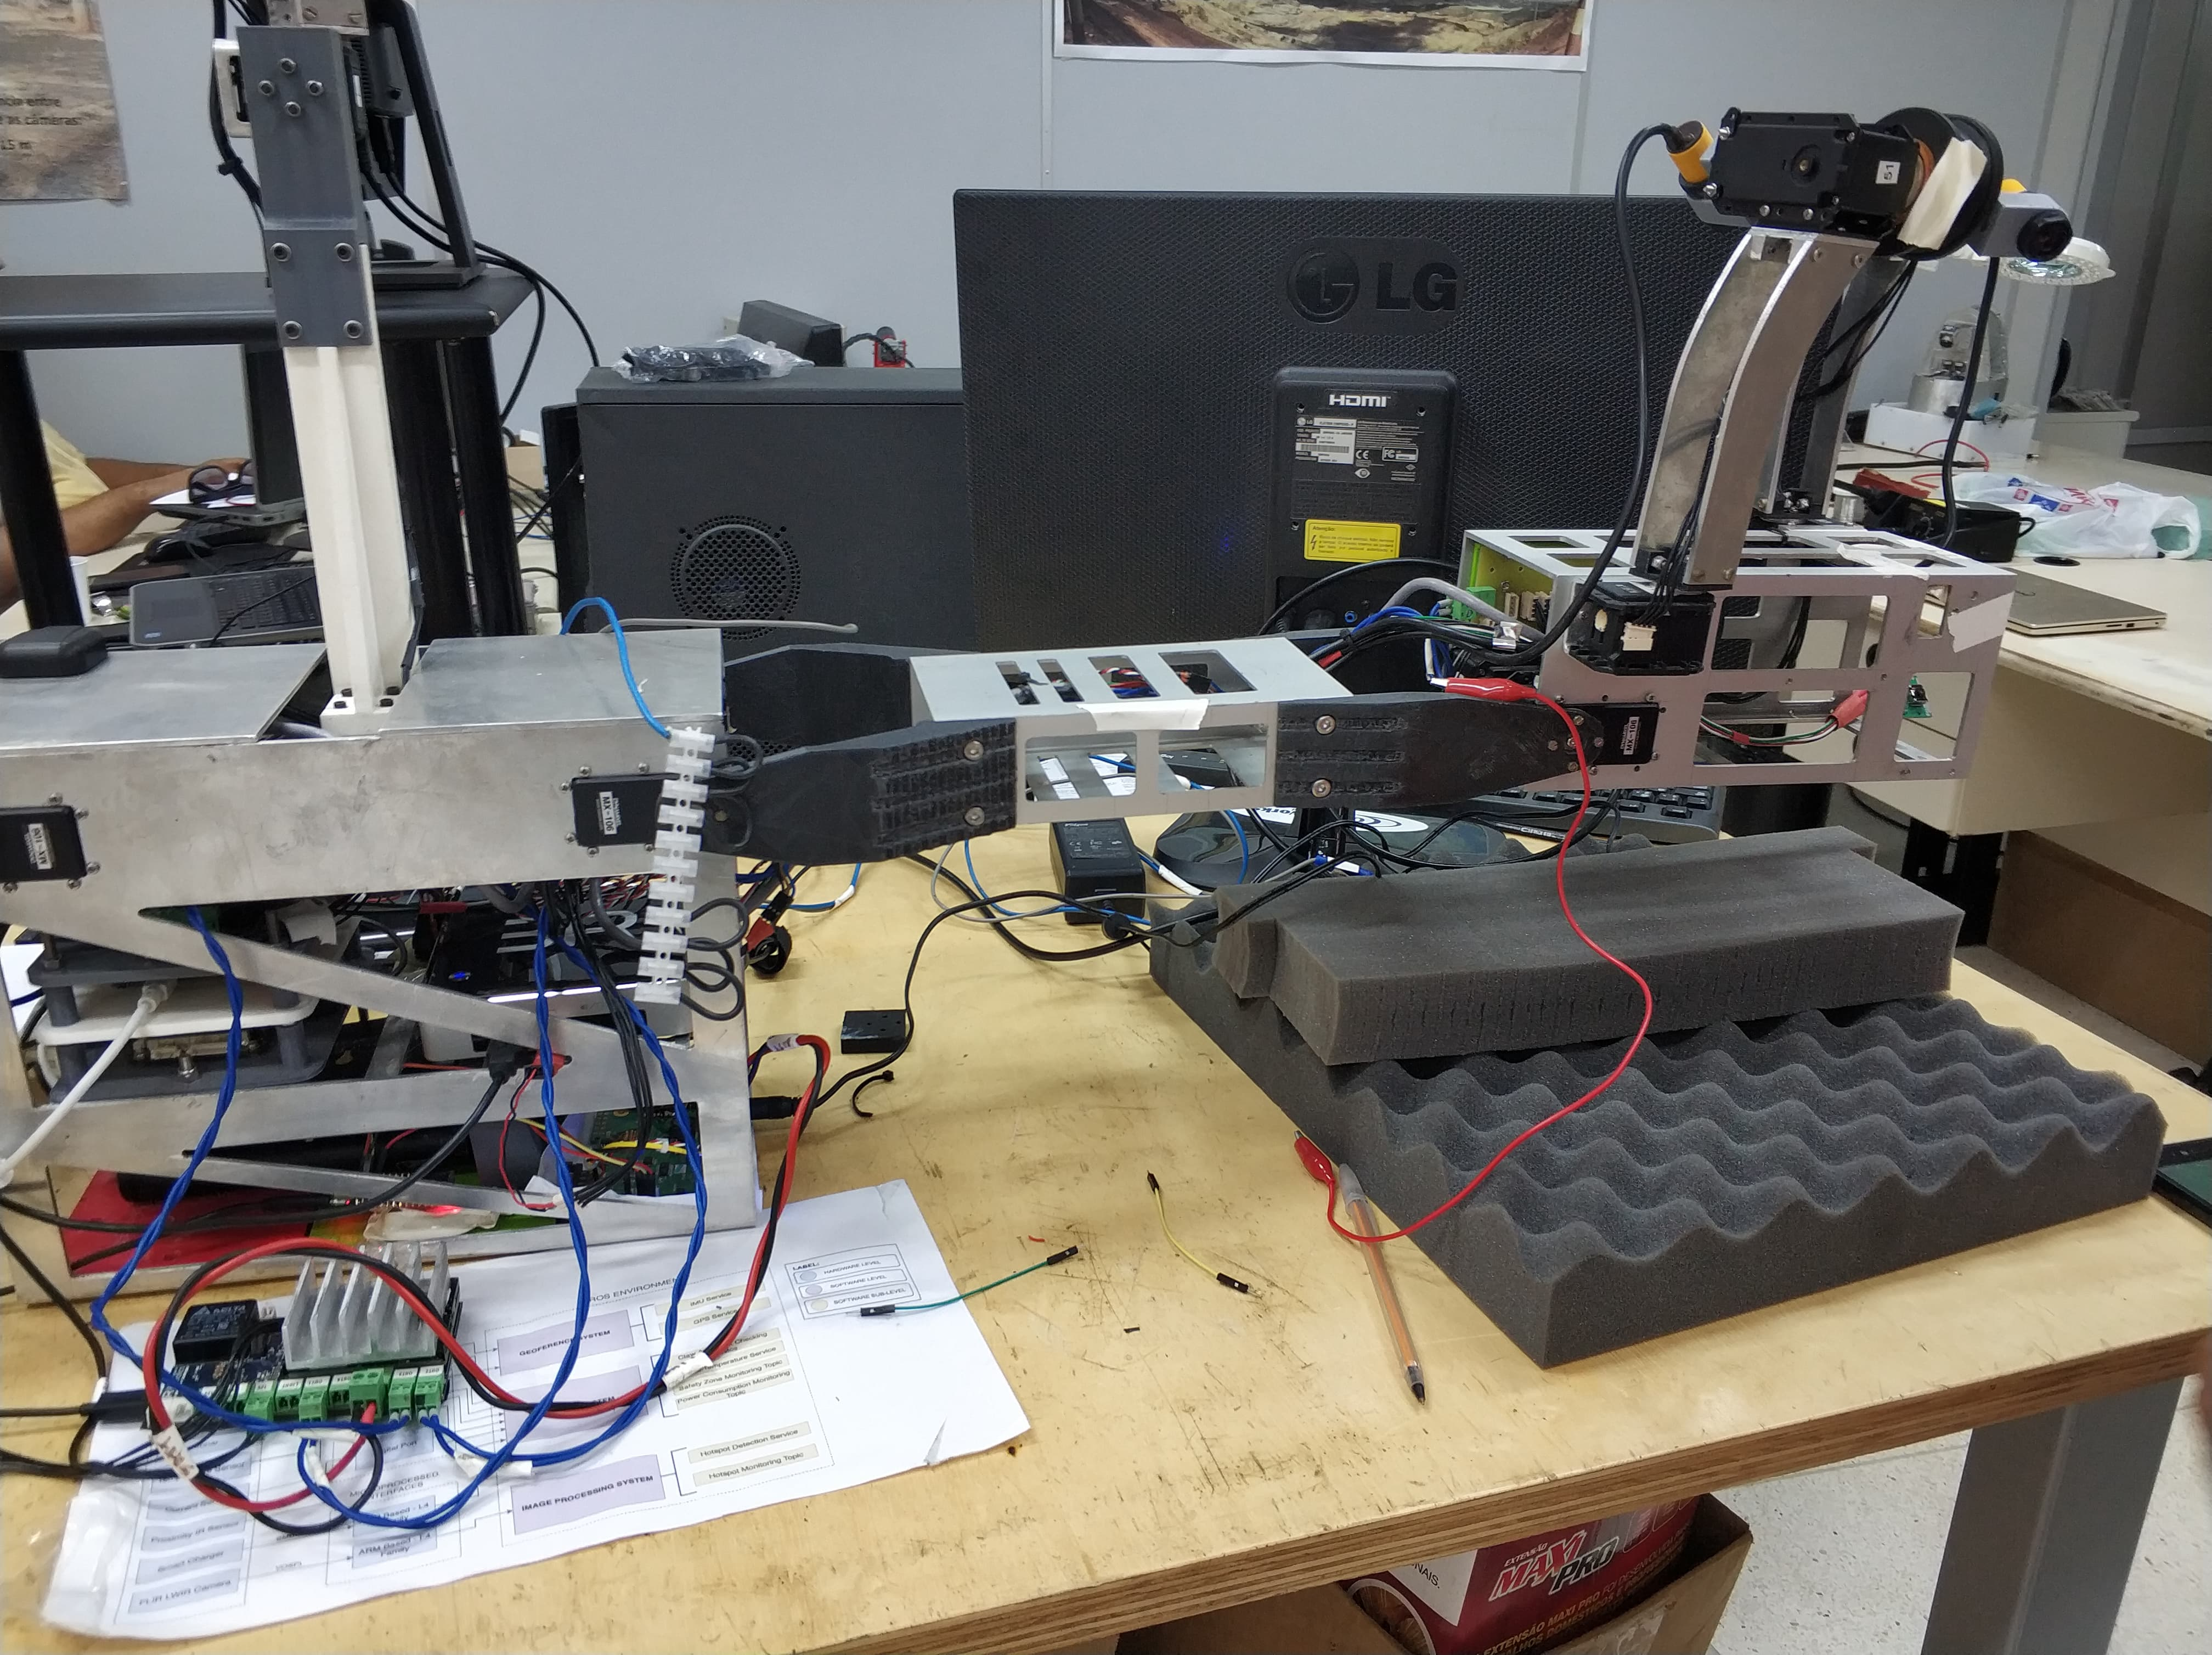
\includegraphics[scale=0.08]{Figures/robo_pior_posicao.jpg}
	\caption{Foto do robô na posição que demanda maior torque}
	\label{fig:robo_pior_pos}
\end{figure}

Verificou-se que o robô respondeu bem com as baterias ficando nesta posição durante 10 minutos por 3 vezes, validando o seu uso e comprovando que os motores a 12V fornecidos pela placa realizam torque suficiente para a carga da estrutura.

\section{Análise Preliminar}\label{sec:anal_prem}







    %\chapter{Título do capítulo}\label{chapter:outro}

As organizações atuam em um ambiente global altamente competitivo, dinâmico, complexo e instável. Tais características denotam cenários de imprevisibilidade, onde todas as suas operações e atividades precisam ser vistas e revistas continuamente. Neste contexto do mundo dos negócios, é de fundamental importância que as organizações busquem estratégias eficazes para suas operações - planejamento, marketing, finanças, produção, qualidade e a logística - por serem cada vez mais importantes e por estarem relacionadas diretamente com as atividades fim dos variados sistemas produtivos.

Busca-se, portanto, reduzir custos em toda cadeia de valor e prover a satisfação dos clientes. Por esta ótica é possível entender o porquê da logística está em evidência na conjuntura atual de mercado. O fato desta ser amparada nos pilares: transportes, gestão de estoques, processamento de pedidos, atividades de apoio e ter como objetivo prover o cliente com os níveis de satisfação desejados pelos mesmos, faz com que a logística assuma um papel fundamental para as organizações: ser um componente capaz de gerar uma vantagem competitiva fundamental, ou seja, providenciar bens e serviços de maneira correta, em tempos e lugares exatos, na condição desejada e em menor custo possível.

Entretanto, quando se fala em melhoria da eficiência operacional na distribuição física, não é suficiente considerar apenas o meio de transporte mais utilizado no Brasil - o rodoviário; é preciso, analisar toda matriz de transporte disponível, para alcançar um serviço capaz de atender satisfatoriamente o canal de vendas. Essa visão considera cada etapa do processo de transporte, procurando sempre identificar as possíveis alternativas, muitas vezes descartadas ou mal exploradas.

Conforme Lambert, Stock e Vantine (1998), estima-se que no Brasil os gastos com atividades logísticas correspondam a 17\% do Produto Interno Bruto (PIB) e, na média, o transporte envolve 60\% dos custos logísticos das empresas. Estes dados justificam a necessidade de um sistema de transporte possuir mecanismos capazes de analisar quais opções de modais apresentam-se mais adequadas ao seu contexto de negócio. Ressalta-se ainda, que a seleção de modais afeta diretamente o preço dos produtos, as condições de entrega e a pontualidade, elementos estes considerados estratégicos para que o sistema alcance seu objetivo.

Segundo os mesmo autores, os cinco principais modais básicos são: rodoviário, ferroviário, aquaviário, dutoviário e aéreo, e sua importância relativa deve ser medida em termos de quilometragem do sistema, volume de tráfego, receita e natureza de composição. Justamente por tais questões que o modal aquaviário se configura como uma alternativa importante para a matriz de transportes brasileira, principalmente quando se fala em cabotagem, devido as características geográficas do Brasil.

Qualquer pesquisa efetuada no Brasil sobre modal aquaviário depara-se imediatamente com a seguinte questão fundamental: por que esse modal logístico é menos usado do que a lógica indicaria? O mesmo é verdade para o modal ferroviário. Por que são tão minguados face ao modal rodoviário? Qual a causa desse "transtorno dos modais", essa terrível modalidade de doença logística que aflige o Brasil e constitui uma de suas mais graves patologias?

Muitos estudos têm analisado essa síndrome de hipertrofia rodoviária e anemias ferroviária e aquaviária. Segundo a COPPEAD-UFRJ, o modal rodoviário responde por cerca de 60% de tudo que é transportado no país, enquanto em países de dimensões territoriais equivalentes ao Brasil, como os EUA e a Rússia, esses percentuais são, respectivamente, 35% e 19%.

Independentemente de comparações entre países, salta aos olhos imediatamente o absurdo de se transportar por caminhão cargas de São Paulo a Fortaleza ou Belém, em trajetos de mais de 3.000 km, quando existe a possibilidade de se usar a cabotagem, mais econômica e menos poluidora.

A considerável literatura técnica que versa sobre cabotagem refere-se quase exclusivamente à carga geral conteinerizada, porque é nessa área que reside o maior potencial de alteração de modal. Em matéria de granéis líquidos e sólidos, a maior parte do que pode ser transportado por cabotagem já o está sendo. Ademais, nesse caso, o transporte dutoviário é geralmente mais indicado.

As lamentações sobre a pouca utilização do modal de cabotagem devem ser entendidas como referentes sobretudo à submodalidade de carga geral. Mas há também absurdas quantidades de caminhões transportando granéis sólidos e líquidos a grandes distâncias nas estradas nacionais. A cabotagem, por sua vez, é parte de uma categoria mais ampla, o modal aquaviário ou hidroviário, dividido em dois submodais: cabotagem e transporte fluvial, esse chamado também de navegação interior, que envolve rios, canais e lagoas.

Portanto, pode-se afirmar que o processo de globalização, o transporte intermodal e as revoluções tecnológicas dos últimos anos na indústria de transporte fluvial resultaram em uma busca maior pela otimização das operações de empresas diretamente envolvidas nesse modal e, principalmente, na expansão das chamadas redes marítimas. No entanto, a falta de dados precisos sobre as relações entre os portos, vem impedindo uma maior aplicação da teoria de redes marítimas, que muitas vezes são analisadas por meio de estudos de caso de empresas ou regiões específicas.

A pesquisa e análise do referencial teórico especializado, na área de redes marítimas, demonstram que a grande maioria dos estudos e produção científica investigam pouco a resolução de problemas específicos sobre essas redes, especialmente observando importantes fatores diretamente relacionados a elas como movimentação de cargas, que interferem de maneira coordenada e agregadora no comportamento individual de cada nó dessa rede, ou seja, os portos.

Assim sendo, as análises de redes marítimas se constituem como um dos maiores campos a serem explorados pela evolução do conceito de redes sociais. Neste sentido, este projeto objetiva analisar a estrutura espacial e dinâmica regional da movimentação de contêineres por cabotagem entre os principais portos na costa brasileira, contribuindo com o estado da arte da seguinte maneira: (1) construindo e analisando redes marítimas, com a utilização de softwares especializados para modelagem computacional dessas; (2) hierarquizando os portos brasileiros através da metodologia AHP e (3) identificando possíveis formações de "clusters" entre os operadores logísticos envolvidos nessas redes através das chamadas constelações competitivas. O resultado da junção dessas análises poderá potencializar positivamente a cabotagem brasileira na obtenção de importantes impactos relacionados à sua gestão.

    %
\chapter{Scenario Definitions and Network Analysis}\label{chpdata}

This chapter illustrates the use of our model to represent a real world population,
summarises the model's options and examines the properties of the underlying small world
network representation for a variety of scenarios. It highlights and contrasts the
model's strengths and weaknesses as compared with the original small world model
\cite{Watts1998} and traditionally used social network models.


\section{Scenarios}

The data used to define the population scenarios for analysis and validation of this
model comes from Brazil. A national study conducted in 2000, evaluated the sexual
behaviour of the Brazilian population and perception of HIV/AIDS \cite{msbrasil2000}. The
study consisted of a face to face interview of 3,600 males and females ageing between 16
and 65 years and living in urban areas of 169 micro regions of Brazil. The micro regions
were defined by the Brazilian 1996 census. The urban population in this age range was
77,018,813 people and the sample region represents a population of 59,872,819 people,
corresponding to 77.7\% of this population.

A similar study was conducted in 2003 by the Brazilian National STD/AIDS programme to
investigate the behaviour of the sexually active population in the past six months, 14
years of age and above \cite{msibope2003}. This second study focused only on sexual
behaviour and safe sex practice of the population; 1,298 face to face interviews were
conducted nationwide.

A further follow-up survey entitled the \emph{Knowledge, Attitudes and Practices of the
Brazilian Population aged between 15 and 54 years} \cite{Szwarcwald2004} expanding on the
first and second was completed in 2004. A total of 6,000 individuals were interviewed,
the sample was stratified according to geographic region (macro-region): 900 interviews
were conducted in the North, South and Centre-West regions, 1,100 in the Northeast region
and 2,200 in the Southeast. In each of the major regions, the sample was carried out in
multiple stages: States; census sectors; and households. The sectors within each of the
States were selected by systematic sampling, with probability proportional to size.

\newpage
The data from the second and the third studies is also available and was used to adjust
the parameters fitted to the first study due to observed sexual behavioural changes
during the four years gap. For clarity the data is not presented here but in Appendix
\ref{chpfitting}. The way that parameters were estimated and the model was fitted is also
described in detail in Appendix \ref{chpfitting}. The following two scenarios will be
used to verify and validate the model as a small world network, illustrate its use to
represent a real world population and the flexibility of the model implementation.

\subsection{Single Group}\label{scenariosingle}

Table \ref{singlegroup} defines a single group representation of the population; this
scenario will be used to illustrate the properties of the social network, the effects of
sexual behavioural change and social interactions on the dynamics of the sexual
transmission of HIV in a small world network.

\begin{longtable}[c]{|p{9cm}|c|}
\caption{Single group scenario definition}\label{singlegroup}\\ \hline
\bfseries Parameters and probability distributions & \bfseries Value (months) \\\hline\hline
\endfirsthead

\multicolumn{2}{c} {{\tablename} \thetable{} -- Continued} \\\hline
\bfseries Parameters and probability distributions & \bfseries Value (months) \\\hline\hline
\endhead
\multicolumn{2}{r}{\emph{Continued on next page}}
\endfoot
\endlastfoot

Population size (\emph{n})      & 3,324  \\\hline
Age distribution                & Weibull(181.47, 267.95, 1.46) \\\hline
Life expectancy                 & 840 (70 years) \\\hline
Proportion of females           & 0.55  \\\hline
Proportion of males             & 0.45  \\\hline
Proportion of homosexual males  & 0.05  \\\hline\hline
HIV prevalence                  & 0.007 \\\hline
HIV lead-time distribution                                    & Weibull(0.13, 47.78, 1.36) \\\hline
HIV testing rate                                              & 0.28 \\\hline\hline
Maximum number of concurrent partnerships                     & 5    \\\hline
Probability of concurrent partnership                         & 0.11 \\\hline
Probability of a casual partnership                           & 0.18 \\\hline
Probability of looking for a sexual partner at any time       & 0.82 \\\hline
Probability of searching own group first for a casual partner & 1    \\\hline\hline
Duration of stable partnerships                                                   & Weibull(141.36, 1.10) \\\hline
Time between stable partnerships                                                  & Gamma(20.20, 1.06) \\\hline
Rate of sexual intercourse for stable partnership per unit of time                & Gamma(4.83, 1.41) \\\hline
Probability of safe sex practice during sexual intercourse for stable partnership & 0.18 \\\hline\hline
Duration of casual  partnerships                                                  & InvNormal(-2.44, 14.49, 49.60) \\\hline
Rate of sexual intercourse for casual partnership per unit of time                & Gamma(5.02, 1.5) \\\hline
Probability of safe sex practice during sexual intercourse for casual partnership & 0.42 \\\hline
\end{longtable}

\subsection{Multiple Groups}\label{scenariomulti}

Table \ref{multigroup} defines a multi group representation of the Scenario
\ref{scenariosingle} population. It is important to notice the overlapping of the group
definition for \emph{under 25} and \emph{married} groups. In this case, being married has
higher priority over age, therefore less than 25 years of age and married individuals are
classified as part of the married sub group. This scenario will be used to evaluate the
effects of inter core group interactions on the dynamics of the sexual transmission of
HIV in a small world network. For simplicity the initial HIV prevalence will be kept
unchanged.

\begin{landscape}
\begin{longtable}[c]{|p{8.1cm}|c|c|c|}
\caption{Multi group scenario definition}\\ \hline
\bfseries \multirow{2}{8.1cm}{Parameters and probability distributions} & \multicolumn{3}{|c|}{\bfseries Groups Definition (months)} \\
\cline{2-4} & \bfseries Married & \bfseries Under 25 & \bfseries Others \\\hline\hline
\endfirsthead

\multicolumn{4}{c} {{\tablename} \thetable{} -- Continued} \\\hline
\bfseries \multirow{2}{8.1cm}{Parameters and probability distributions} & \multicolumn{3}{|c|}{\bfseries Groups Definition (months)} \\
\cline{2-4} & \bfseries Married & \bfseries Under 25 & \bfseries Others \\\hline\hline
\endhead

\multicolumn{4}{r}{\emph{Continued on next page}}
\endfoot
\endlastfoot
\label{multigroup}
Population size (\emph{n})      & 1422 & 794 & 1108 \\\hline
Age distribution                & \small{Weibull(182.3, 336.28, 2.29)}& \small{LogNormal(143.95, 95.05, 36.99)} & \small{InvNormal(242.15, 246.94, 621.89)}\\\hline
Life expectancy (70 years)      & 840 & 840 & 840 \\\hline
Proportion of females           & 50\%   & 45.7\% & 62.4\% \\\hline
Proportion of males             & 50\%   & 54.3\% & 37.6\%\\\hline
Proportion of homosexual males  & 5\%    & 5\%    & 5\%  \\\hline\hline
HIV prevalence                  & 0.007   & 0.007   & 0.007 \\\hline
HIV lead-time distribution      & Weibull(64.26, 1.63) & Weibull(71.79, 1.61) & Weibull(64.26, 1.63) \\\hline
HIV testing rate                & 16.34\% & 11.71\% & 18.29\% \\\hline\hline
Maximum number of concurrent partnerships                     & 5 & 5 & 5 \\\hline
Probability of concurrent partnership                         & 0.06 & 0.21 & 0.14 \\\hline
Probability of a casual partnership                           & 0.06 & 0.40 & 0.27 \\\hline
Probability of looking for a sexual partner at any time       & 1 & 0.78 & 0.64 \\\hline
Probability of searching own group first for a casual partner & 0.4 & 0.8 & 0.7 \\\hline\hline
Duration of stable partnerships                                                   & Weibull(198.19, 1.55) & LogNormal(29.77, 37.2) & Weibull(89.74, 1.01) \\\hline
Time between stable partnerships                                                  & Gamma(20.16, 1.07) & Weibull(14.89, 1.10) & Gamma(24.38, 1.03) \\\hline
Rate of sexual intercourse for stable partnership per unit of time                & Gamma(4.71, 1.51)  & Gamma(6.5, 1.06)     & Gamma(5.09, 1.34) \\\hline
Probability of safe sex practice during sexual intercourse for stable partnership & 0.11 & 0.47 & 0.21 \\\hline\hline
Duration of casual  partnerships                                                  & Gamma(8.84, 1.14) & Gamma(5.25, 1.03) & LogNormal(9.16, 14.61) \\\hline
Rate of sexual intercourse for casual partnership per unit of time                & Gamma(5.01, 1.58) & Gamma(7.1, 1.1) & Gamma(5.31, 1.39)  \\\hline
Probability of safe sex practice during sexual intercourse for casual partnership & 0.12 & 0.55 & 0.42 \\\hline
\end{longtable}

\begin{longtable}[c]{|c|c|c|c|}
\caption{Multi group default mixing matrix}\\ \hline
\label{multimixmat}
$\Rightarrow \oslash \Rightarrow $ & Married & Under 25 & Others \\\hline
& & & \\
Married  & x       & 0.5      & 0.5    \\
& & & \\\hline
& & & \\
Under 25 & 0.5     & x        & 0.5    \\
& & & \\\hline
& & & \\
Others   & 0.5     & 0.5      & x      \\
& & & \\\hline
\end{longtable}

\end{landscape}

The population mixing matrix defined in Table \ref{multimixmat} is given as default and
assumes that the flow of people between any two groups is the same on both directions.
However this is not the case for most real world situations and one should tune these
parameters in order to give a more realistic representation of the direction of external
interactions between different core groups' populations.

\subsection{HIV Infection}

The variables required by the model to represent the transmissibility and natural history
of the STD infection have been specified in section \ref{stddefsection}. Table
\ref{hivdefinition} defines the characteristics of the HIV transmission and progress from
infection to AIDS death without HAART intervention.

\begin{longtable}[c]{|p{8cm}|c|c|}
\caption{Transmissibility and natural history of HIV infection}\\\hline
\label{hivdefinition}
\textbf{Probability of HIV Transmission}     & \textbf{Value} & \textbf{References}  \\\hline
Female to Male                               & 0.002 &  \cite{Donovan2000,Royce1997} \\\hline
Male to Female                               & 0.003 &  \cite{Donovan2000,Royce1997} \\\hline
Male to Male                                 & 0.010 &  \cite{Donovan2000,Royce1997} \\\hline
\multicolumn{3}{|l|}{\textbf{Infection Characteristics}}\\\hline
Lifelong infection?                          & Yes   &  \\\hline
Duration of infection                        & N/A   &  \\\hline
Allow reinfection?                           & No    &  \\\hline
Mortality rate                               & 98\%  & \cite{UNAIDSRG2002} \\\hline
\multicolumn{3}{|l|}{\textbf{Natural History of HIV infection}}\\\hline
Progression from HIV infection to AIDS death & Weibull (126.12, 2.38) & \cite{UNAIDSRG2002} \\\hline
\end{longtable}


\subsection{Global Settings}\label{globalsettings}

The model's global configuration guides how the simulation behaves during run-time as
well as defines the constraints for calculation of the network global efficiency, length
of simulation warm-up, distribution of the initially infected individuals within the
population and the network structure. Table \ref{hivacsimconfig} defines the default global settings that
will be used throughout the model evaluation and validation. Changes to this global
configuration will be explicitly stated when they are required for the demonstration of a
specific property or condition.

\begin{longtable}[c]{|p{10cm}|c|c|}
\caption{HIVacSim global configuration and network structure definition}\\\hline
\label{hivacsimconfig}
\textbf{Simulation Properties}     & \textbf{Value} & \textbf{References}  \\\hline
Clock                                       & Month & \ref{hivacsim} \\\hline
Duration (12 years)                         & 144   & \ref{hivacsim} \\\hline
Replications (Runs)                         & 100   & \ref{hivacsim} \\\hline
\multicolumn{3}{|l|}{\textbf{Global Efficiency Calculation}}\\\hline
Switch algorithm at small world probability \emph{p} value & 0.13      & \ref{netinfo}\\\hline
Maximum network size for numerical calculation      & 500       & \ref{netinfo}\\\hline
Size of the geodesic sample for estimation          & 400       & \ref{netinfo}\\\hline
\multicolumn{3}{|l|}{\textbf{Warm-up \ref{warmup} and Initial Infection}}\\\hline
Duration (2 years)                                  & 24     & Table \ref{warmupconfig} \\\hline
Minimum number of concurrent partnerships           & 2      & Table \ref{warmupconfig} \\\hline
Probability of concurrent partnership               & 0.5    & Table \ref{warmupconfig} \\\hline
Distribution of the initial infection               & Clustered & \ref{initinfdist}\\\hline
\multicolumn{3}{|l|}{\textbf{Network Structure}}\\\hline
Maximum size of the acquaintances list              & 50     & \ref{listsize}\\\hline
$\beta$ (maximum number of trials)                  & 1      & \ref{searchrel}\\\hline
Degrees of separation                               & 3      & \ref{searchrel}\\\hline
Expected number of people in one's neighbourhood    & 50     & \ref{structure}\\\hline
Radius of the real world (earth)                    & 6378   & \ref{structure}\\\hline
Network topology                                    & Sphere & \ref{structure}\\\hline
\end{longtable}

The network structure settings are defined at group level and as such they may assume
different values according with the size of each group's population. The values provided
in Table \ref{hivacsimconfig} for size of the acquaintances list and neighbourhood are
used for solving Equations \ref{egnofriends} and \ref{solvedistance} respectively within
each group definition. The maximum number of trials is also dependent on the population
size and therefore will have a similar effect on the searching for relationships
(\ref{searchrel}, b).

\section{Small World Network Properties}\label{swnproperties}

The characteristics and measurements of small world networks are described in Section
\ref{swnetworks}. This section evaluates the strengths to which the HIVacSim model
conforms to the general theory of small world networks. Scenario \ref{scenariosingle}
will be used for verification and validation of the small world model in this and the
next chapter unless specified otherwise. 15 replications of each experiment are used
throughout this exercise to produce the plots, error bars and to define confidence
limits.

The original small world model of Watts and Strogatz \cite{Watts1998} can be quantified
by two simple statistics: the clustering coefficient \emph{C} for measuring local density
and the mean geodesic length \emph{L} for measuring the global separation. A small world
network is defined as a broad region between regularity and randomness in which the
network is highly clustered and has a short path length. As discussed in Sections
\ref{smgraphs} and \ref{geodesic}, the original formulation of the mean geodesic length
by Watts and Strogatz \cite{Watts1998} is valid only for fully connected networks. This
is not always the case in the real world where not everyone has friends or is involved in
a sexual partnership all the time.

Figure \ref{connected} shows the frequency of fully connected network occurrences found
experimentally in this model as a function of the network randomness parameter \emph{p}
(\emph{x axis has multiple scales}). This clearly illustrates the limitation of the
original small world model formulation and supports the adoption of a more consistent and
meaningful notation (\ref{netefficiency}) to quantify the characteristics of a small
world network.
\begin{figure}[h]
\includegraphics[width=\textwidth]{connected}
\caption{Frequency of fully connected sexual network occurrences} \label{connected}
\end{figure}

Figure \ref{originalswn} gives the small world network characteristics \emph{L} and
\emph{C} evaluated according to the original formulation of Watts and Strogatz
\cite{Watts1998}. Note that the \emph{L} values have been calculated only for the
occurrences of a fully connected network. Nevertheless the small world effect is clearly
visible. At just a small amount of randomness $(p \sim 0.1)$, \emph{L} has almost reached
its minimum value, yet \emph{C} is about half of its maximum value.
\begin{figure}[ht]
\begin{center}
\includegraphics{originalswn}
\caption{Characteristics of a small world network} \label{originalswn}
\end{center}
\end{figure}

Another global measure depending upon full network connectivity is the diameter, defined
as the length of the longest geodesic (\ref{geodesic}). This measure has a close relation
with the mean geodesic length and therefore can be evaluated only for fully connected
networks. Figure \ref{diameter} shows the small world effect on network diameter.
\begin{figure}[!h]
\includegraphics{diameter}
\caption{Small world effect on network diameter} \label{diameter}
\end{figure}

\subsection{Network Efficiency}\label{netefficiency}

The concept of efficiency on small world networks has been introduced by Latora and
Marchiori \cite{Latora2001} for measuring the global and local efficiency of a network
(\ref{smnefficiency}); these measures are denoted by $E_g$ and $E_l$ respectively. From
this perspective a small world network can be rephrased as a network with high global and
high local efficiency, therefore exchanging information very efficiently both on a global
and on a local scale. Figure \ref{efficiency} shows the HIVacSim model's efficiency.
These values compare well with those provided by Latora and Marchiori \cite{Latora2001},
and therefore we concluded that the HIVacSim network model indeed represents a small
world network.
\begin{figure}[h]
\includegraphics[width=\textwidth]{efficiency}
\caption{HIVacSim model's global and local efficiency} \label{efficiency}
\end{figure}

The short paths represented by the global efficiency, provide high-speed communication
channels between distant parts of the network, thereby facilitating any dynamical process
that requires global coordination, transmission of information or propagation of
infectious disease. The local efficiency provides short distance communication, enabling
high-speed propagation of information or disease through local clusters within the
population.

The network efficiency has a good agreement with the original small world model
formulation due to Watts and Strogatz \cite{Watts1998} by reporting a normalised
$1/E_g(p)$ and $E_l(p)$ as shown in Figure \ref{efficiencyswn}.
\begin{figure}[h]
\begin{center}
\includegraphics{efficiencyswn}
\caption{Network efficiency as the original small world characteristics}
\label{efficiencyswn}
\end{center}
\end{figure}

Figure \ref{efficiencyswn} compares well with Figure \ref{originalswn}, produced using
the original formulation of the small world characteristics. The small discrepancies
between global efficiency and \emph{L} can be attributed to the fact that the values for
\emph{L} in Figure \ref{originalswn} have been calculated using only a fraction of the
data produced by the experiment due to its network connectivity requirement, which is not
the case for global efficiency.


\subsection{Clustering Coefficient}\label{swnclustering}

The small world clustering coefficient \emph{C} defined in Section \ref{clusteringcoef},
measures the overlapping of acquaintances within the population. This measure can be
calculated numerically for the fully connected regular (\ref{latticegraphs}), the random
(\ref{randomgraph}) and the original small world network models (\ref{clusteringcoef}).
However for disconnected networks there is no deterministic formulation and therefore
this quantity has been evaluated through Monte Carlo simulation. Figure \ref{clustering}
compares the clustering coefficient of our small world model with results obtained by
deterministic evaluation of equivalent regular and random networks.
\begin{figure}[ht]
\includegraphics[width=\textwidth]{clustering}
\caption{Small world clustering coefficient} \label{clustering}
\end{figure}

As shown in Figure \ref{connected}, regular networks are less likely to be fully
connected due to the lack of concurrency and absence of long distance connectivity among
individuals within the population. This behaviour has a direct impact on the clustering
coefficient of the small world network as shown in Figure \ref{efficiencyswn}. However
real world networks, and in particular sexual networks, rarely fall in this category as
being regular and fully connected at the same time. Therefore we conclude that the
clustering coefficient of our small world network model approaches both extremities of
the theoretical spectrum for regularity and randomness with good accuracy and precision,
so it is consistent with the general definition of the small world network theory.


\subsection{Degree Distribution}

The study of degrees has received enormous attention in social networks and as a
consequence, it is one of the most popular terms in the sociology literature. It refers
to the number of social connections that one possesses, the number of partners at a point
in time and so on. From a small world perspective, the degree distribution quantifies the
size of the lists of acquaintances, the popularity of individuals within the network.
Figure \ref{degreeavg} shows the small world effects on the average degree of the
individuals within our model, a non-linear relation between randomness and average degree
can be observed.
\begin{figure}[h]
\includegraphics{degreeavg}
\caption{Small world effect on the average degree distribution} \label{degreeavg}
\end{figure}

Application of degrees is as common in graph theory as it is in social networks. It forms
the basis of the network \emph{centrality}, a measure of the varying importance of the
individuals in a network according to some predefined criterion, a coefficient of the
popularity of an actor, also known as degree centrality (\ref{netcentrality}). Degrees
were also the basis of the reverse small world experiment \cite{Killworth1978}.

The degree distributions of the original small world models have been defined through a
set of equations in Section \ref{swndegreedist}. However, they do not match most real
world networks very well since this was not a goal of the original model in the first
place. We provide empirical results showing the small world effect on degree distribution
of individuals within our model.

Figures \ref{degreepdf} and \ref{degreecdf} give the degree probability density function
(PDF) and cumulative distribution function (CDF) respectively. They clearly show the
small world effect on the degrees distribution of the population as a function of the
small world randomness parameter \emph{p}. As the randomness value of \emph{p} increases,
the location and shape of the degree distributions also change following a non-linear
scale as can be observed by looking at the degree CDF.

\begin{figure}[ht]
\includegraphics{degreepdf}
\caption{Empirical degree probability density function (PDF)} \label{degreepdf}
\end{figure}

\begin{figure}[ht]
\includegraphics{degreecdf}
\caption{Empirical degree cumulative distribution function (CDF)} \label{degreecdf}
\end{figure}
\clearpage

\section{Topology of a Small World Network}\label{topology}

Traditional analysis of social networks as it appears in well known works such as
Wasserman and Faust \cite{Wasserman1994}, has focused almost solely on static structure
(\ref{dynamicsw}). It fails to understand how individuals interact within a dynamic
social structure, how the network structure itself is transformed by the actions of the
actors and how the network efficiency will change through time \cite{Watts1999}. In a
sexual social network, actors have different preferences and desires; however their
actions and behaviour must be accepted or shared by their neighbours and partners in
order for them to be socially accepted. Acceptance therefore is a key strategy and actors
will change their behaviour, transform their clusters and dynamically reorganise the
global network in order to achieve their goals.

The network topology defines the shape and layout of a population. The way in which
different individuals in a social network are connected to each other and how they
communicate, propagate information or contagious disease through the network boundaries
are partly influenced by the network's topology. As described in Section \ref{structure},
HIVacSim model provides three topologies:

\parskip=0pt
\begin{itemize}
    \item \emph{Free} -- a network where no geographical considerations are made, people are
    close to each other by social distances. This is typical of traditional social
    networks and epidemiological models with no geographical considerations;
    \item \emph{Circle} -- the original small world networks topological model of Watts and
    Strogatz \cite{Watts1998}, where the population lives in a lattice ring with
    periodic boundary conditions;
    \item \emph{Sphere} -- a topological network introduced by this model as an alternative
    and more realistic representation of the real world where people live on the surface
    of a sphere.
\end{itemize}
\parskip=\baselineskip

In order to quantify the effects of topology on small world network models, we consider
the network efficiency as the baseline for analysis. The experiment consists of running
the HIVacSim model using Scenario \ref{scenariosingle} for each topology, gradually
increasing the network randomness parameter \emph{p} from regularity to randomness, and
evaluating the network efficiency (HIV Prevalence) for each experiment at the end of 144
months (12 years).

An important point about this experiment is the initial distribution of the infected
population, or the origins of the information to be transmitted through the network
connections. As defined in Section \ref{initinfdist}, this model provides two options for
distributing the initial infected individuals or the sources of information within a
network: \emph{uniform} or \emph{clustered}. These initial distributions define the two
scenarios for the topological analysis of our small world network model.

\subsection{Uniform Initial Distribution}

The initially infected individuals or sources of knowledge are uniformly distributed
within the population. This mimics the traditional social networks and epidemiological
models with no geographical considerations. In this regime, the probability of meeting an
infected individual geographically close to someone is the same as anywhere else in the
network. Therefore topology should have no influence on network efficiency because the
information or disease is already widely spread within the population as illustrated in
Figure \ref{uniforminf}. In such a case, one is likely to get infected or acquire the
knowledge from anywhere in the network with the same probability, independent of network
topology or one's geographical location. Figure \ref{topologyuniform} shows the effect of
topology on network efficiency for this experiment.
\begin{figure}[h]
\includegraphics[width=\textwidth]{topologyuniform}
\caption{Network efficiency by topology with uniform distribution}
\label{topologyuniform}
\end{figure}

The differences on network efficiency between topologies are negligible and the errors
bars clearly confirm that no conclusive difference exists. The topology has no effect on
network efficiency when the initially infected individuals or information holders are
uniformly distributed within the network. In such a case, a \emph{topology free network}
should be used as it represents the traditional structure of epidemiological models and
provides an efficient computation time compared with the other two topologies
(\ref{computetime}). Figure \ref{topologyudifference} shows that there is no clear
pattern of topological differences on network efficiency for this scenario. For clarity a
smoothed line has been included to highlight the irregularity of the differences between
topologies.
\begin{figure}[h]
\includegraphics[width=\textwidth]{topologyudifference}
\caption{Topological differences on network efficiency with uniform distribution}
\label{topologyudifference}
\end{figure}

This experiment illustrates the limitations of social networks and epidemiological models
that ignore the dynamics of information and infectious diseases spread through geography.
Life experience suggests that this knowledge is not easy to find, we need to compete and
move to have access to good universities, subscribe to scientific journals, pay for
datasets and so on. Information holders are not uniformly distributed. The spread of
infectious diseases on the other hand can vary enormously by geography. Take for example
the recent SARS epidemic in the Far East where geographical boundaries were effectively
used by health authorities and governments in order to isolate and control the spread of
the virus.

\newpage
In the case of infectious agents with a long incubation period such as HIV, it is
difficult to identify the source of infection and therefore geographical boundaries are
not efficient. Although HIV has been known for more than 20 years, its prevalence
worldwide still varies enormously by continent, country, city, community, etc.  This is
clear evidence that geography must be taken into account when trying to model the
dynamics of social networks and the spread of infectious diseases.


\subsection{Clustered Initial Distribution}

The initially infected individuals or sources of information are distributed by
geographical clusters within the population as shown in Figure \ref{nonuniforminf}. In
this case, the probability of meeting an infected individual geographically close to
someone will depend upon one's social and geographical location within the network.
Information or infectious diseases are dynamically transmitted within the network
geographically through social interactions. Figure \ref{topologynuniform} shows the
effects of topology on network efficiency for a clustered initial distribution.
\begin{figure}[h]
\includegraphics[width=\textwidth]{topologynuniform}
\caption{Network efficiency by topology with clustered distribution}
\label{topologynuniform}
\end{figure}

This result shows that within a dynamic clustered initial configuration, topology matters
and has a distinct effect on network efficiency. It is important to notice that for $p
>\sim 0.8$ the topological effects become inconclusive. This is caused by the amount of
randomness added to the network interactions as it approaches its maximum value at $p =
1.0$. At this point we have a random network and the three topologies effectively
converge to the same network efficiency as expected.

Topology has a clear effect on network efficiency and should not be overlooked. The
\emph{circle topology} clearly has the lowest network efficiency. \emph{Topology free}
has the highest network efficiency, however it completely ignores the geographical
distribution of individuals and consequently is not a realistic representation of the
real world. \emph{Spherical topology} provides an intuitive representation of the real
world and its network efficiency lies between regularity (circle) and randomness (free).
Figure \ref{topologynudifference} gives a different view of the convergence to a random
network and shows how the topology affects the patterns of network efficiency.
\begin{figure}[h]
\begin{center}
\includegraphics[width=\textwidth]{topologynudifference}
\caption{Topological differences on network efficiency with clustered distribution}
\label{topologynudifference}
\end{center}
\end{figure}

Table \ref{topologysummary} summarises the average difference between topologies on
network efficiency for a clustered initial distribution of infection or source of
information. It numerically quantifies the overall topological differences shown in
Figure \ref{topologynudifference} and enforces the importance of topology on
epidemiological and dynamic networks modelling.

\begin{longtable}[c]{|l|c|c|}
\caption{Summary of topological effects on network efficiency}\\\hline
\label{topologysummary}
\textbf{Topologies} & \textbf{Average difference} & \textbf{Standard deviation}  \\\hline
Free to Circle      & 16.66\%   &   0.84\% \\\hline
Free to Sphere      & 5.07\%    &   0.89\% \\\hline
Sphere to Circle    & 12.43\%   &   1.12\% \\\hline
\end{longtable}


\subsection{Computation Times}\label{computetime}

The average simulation run-time for each interaction of HIVacSim using Scenario
\ref{scenariosingle} is affected by both the network topology and the small world
randomness parameter \emph{p }. A laptop with an Intel Pentium Mobile processor 1.6GHz,
2Mb of cache and 512GB of memory was used to run the experiments presented in this
thesis. Figure \ref{runtime} shows a summary of the simulation run-times.
\begin{figure}[h]
\includegraphics[width=\textwidth]{runtime}
\caption{HIVacSim run-times by topology} \label{runtime}
\end{figure}

Topologies \emph{free} and \emph{circle} have identical computational efficiency for each
value of network randomness parameter \emph{p}. However a \emph{free} topology is
preferred over the \emph{circle} as it mimics the structure of traditional
epidemiological and social networks models with no geographical considerations. The
\emph{spherical} topology however gives a better representation of the real world and the
additional computational expense is very much worthwhile.

It is important to notice that the run-times presented in Figure \ref{runtime} are for
100 replications (\ref{globalsettings}) of Scenario \ref{scenariosingle}, in order to
provide statistical evidence for comparison of results. However in practice, less
replication would be needed for simulation experiments (e.g. 10) and therefore the
run-times should be around 1/10 of the quoted values.

    %\chapter{Epidemiological Verification}\label{chpvalidate}

\parskip=15pt
This chapter describes the use of HIVacSim model for representing, examining and solving
real world problems. The effects of living in a small world, sexual behaviour changes and
social interactions on the dynamics of HIV transmission are verified and validated
against existing models and related published data in the literature. The use of
preventive HIV vaccine intervention to control the HIV pandemic is evaluated
experimentally, though no HIV vaccine is available at the time of this writing.

In the previous chapter, we showed the importance of topology on networks and
epidemiological models (\ref{topology}). The \emph{spherical topology} provides a good
representation of the real world and will be used as the default network topology for the
rest of this thesis. The initial distribution of infection within a population must not
be overlooked when modelling the dynamics of disease propagation through networks. It not
only influences the network efficiency between topologies but also within the same
topology. Figures \ref{initdistprevalence} and \ref{initdistincidence} show the effect of
the initial distribution of infection on HIV transmission as the epidemic progresses over
time in a spherical topology (though the results are point values, we have for clarity
used a continuous graph).
\begin{figure}[h]
\includegraphics{initialdistprevalence}
\caption{Effects of the initial distribution of infection on HIV prevalence}
\label{initdistprevalence}
\end{figure}
\parskip=\baselineskip

\begin{figure}[ht]
\includegraphics{initialdistincidence}
\caption{Effects of initial distribution of infection on HIV incidence}
\label{initdistincidence}
\end{figure}

The effects of the initial distributions of infection as well as that of a small world
are evident. At a low level of randomness $(p < 0.4)$, which includes the relevant region
for HIVacSim (see Figure \ref{connected}), the gap between random and clustered initial
distributions of infection remains wide for longer than otherwise due to the clustering
property of the network. As the network randomness increases beyond this level, the
difference between initial distributions decreases faster as the global network
efficiency starts to converge to that of a random network. This result confirms the
importance of geography and shows the effects of the initial distribution of infection on
the propagation of an epidemic within a dynamic small world network.


\section{Small World Effects on Sexual Transmission of HIV}\label{sweffecthiv}

In order to quantify the effects of a small world network on the sexual transmission of
HIV, we use Scenario \ref{scenariosingle}, where we gradually increment the probability
of a casual partnership (small world randomness probability \emph{p}) from regularity $(p
= 0.0)$ to randomness $(p = 1.0)$ and evaluate the development of the HIV epidemic over
time for each experiment.  Figures \ref{swneffectprevoriginal} and
\ref{swneffectincidoriginal} summarise the results for this experiment by showing the
small world effect on the HIV prevalence and HIV incidence respectively as the epidemic
progresses over time in a dynamic network.

\begin{figure}[ht]
\includegraphics[width=\textwidth]{swneffectprevoriginal}
\caption{Small world effect on HIV prevalence} \label{swneffectprevoriginal}
\end{figure}
\begin{figure}[ht]
\includegraphics[width=\textwidth]{swneffectincidoriginal}
\caption{Small world effect on HIV incidence} \label{swneffectincidoriginal}
\end{figure}
\clearpage

The results show that the small world randomness parameter (probability of casual
partnership) directly affects the speed of the HIV transmission. However the rate of
change on the network randomness value does not have a linear effect on HIV transmission,
as can be observed. For example, an increase of 0.1 in the network randomness $(0.0
\rightarrow 0.1)$ results in a 33\% increase in HIV prevalence and a 42\% in HIV
incidence after 12 years compared with the regular network as the baseline.

The slow decrease in HIV prevalence over time in Figure \ref{swneffectprevoriginal} is
explained by the number of AIDS related deaths within the population. The growth rate of
the HIV epidemic increases very fast during its initial phase. In the absence of
treatment intervention to improve and extend the lives of those HIV infected individuals,
the AIDS symptoms will develop naturally and kill those infected. Figure
\ref{swneffectnodeath} confirms this argument by showing the HIV prevalence for the
scenario above but now assuming that HIV infection will not lead to AIDS and subsequent
death. In the model, the \emph{HIV mortality rate} is set to \emph{zero} (see Table
\ref{hivdefinition}).

\begin{figure}[ht]
\includegraphics[width=\textwidth]{swneffectnodeath}
\caption{Small world effect on HIV prevalence without AIDS deaths}
\label{swneffectnodeath}
\end{figure}

This result shows the importance of treatment for those infected with HIV and highlights
the world's need to understand the long term consequences of widely accessible HAART
treatment for the HIV epidemic as a whole. A balance between prevention and treatment is
crucial, the effectiveness of HAART might be less important than behavioural influences
on the progress of the HIV epidemic \cite{Dangerfield2001}.

In order to illustrate the consequences of treatment interventions in the HIV epidemics,
we experimentally evaluate the efficacy of a HAART programme with 100\% HIV positive
population coverage (infectivity is kept unchanged). Assuming that through HAART we could
double the life expectancy of those infected individuals, Figure \ref{swneffecthaart}
shows the effects of HAART on the HIV prevalence as the epidemic progresses over time
with different levels of randomness in the network.

\begin{figure}[h]
\includegraphics[width=\textwidth]{swneffecthaart}
\caption{Effects of HAART intervention on HIV prevalence} \label{swneffecthaart}
\end{figure}

This result clearly shows that widely accessible HAART treatment dramatically increases
the number of HIV positive individuals within the general population over time.
Governments and health authorities must be aware of the long term consequences of such
HAART programmes in order to improve the planning and management of resources to prevent
HIV infection in the first place and make the life of those infected more human and
comfortable.

The small world network efficiency peaks at about 90\% of randomness and not at 100\% as
one might expect (see Figures \ref{swneffectprevoriginal} to \ref{swneffecthaart}). This
rather curious occurrence is explained by the difference in sexual behaviour regarding
safe sex practices between stable (18\%) and casual (42\%) partnerships. Figures
\ref{swneffectprevcondom} and \ref{swneffectincidcondom} confirms this argument by
showing the HIV prevalence and incidence for the scenario above by now assuming the same
rate of safe sex practice (18\%) for both casual and stable partnerships.

\begin{figure}[ht]
\includegraphics[width=\textwidth]{swneffectprevcondom}
\caption{Same rate of safe sex practice effects on HIV prevalence}
\label{swneffectprevcondom}
\end{figure}
\begin{figure}[ht]
\includegraphics[width=\textwidth]{swneffectincidcondom}
\caption{Same rate of safe sex practice effects on HIV incidence}
\label{swneffectincidcondom}
\end{figure}
\clearpage

The small world network theory may explain in part why HIV has managed to spread itself
to every corner of the world, infecting and killing people from all ethnic and social
backgrounds, surviving like no other disease has ever done in the same proportion and
time scale. An infectious disease or information needs only a small amount of randomness
$(p \sim 0.2)$ in the network interactions in order for it to efficiently propagate on a
local and global scale.

By examining the small world effects on the HIV epidemic for the original population
definition shown in Figures \ref{swneffectprevoriginal} and \ref{swneffectincidoriginal},
one can observe that there is no major increase in network efficiency or epidemic growth
after 12 years for randomness parameter $p > 0.5$. At $p \approx 0.5$, the network has
already reached over 70\% of its maximum efficiency $(p \sim 0.9)$. These results were
corroborated by Kuperman and Abramson \cite{Kuperman2001} for a SIR model using the
original small world model.

Figure \ref{smallpertubation} shows that small perturbations in the system such as the
experimental changes in safe sex practices illustrated by Figures
\ref{swneffectprevcondom} and \ref{swneffectincidcondom}, can have an unpredictable
effect on the network efficiency and therefore on the course of the HIV epidemic. Error
bars used in plots throughout this chapter represent a 95\% confidence interval for the
mean.
\begin{figure}[h]
\includegraphics[width=\textwidth]{smallpertubation}
\caption{The effects of small perturbations on network efficiency}
\label{smallpertubation}
\end{figure}
\clearpage

This result highlights the importance of preventive intervention strategies such as sex
education and free condoms to fight the HIV pandemic. It also illustrates the network
sensitivity to small behaviour changes among individuals and shows how such changes are
dynamically propagated within the network.

The magnitude of the small world effect on the HIV epidemic can be quantified by both
prevalence and incidence as above. This experiment highlights the flexibility of the
HIVacSim model in representing different aspects of the infectious disease in question,
identifying and quantifying the causes leading to the transmission and evaluating the
consequences of small behavioural changes for the future development of the epidemic.


\section{HIVacSim as a Compartmental Model}\label{hivacsimsir}

The basic compartmental models of disease spread, also known as SIR models are still the
standard in epidemiology (\ref{sirmodels}). This traditional family of models are
represented within HIVacSim by the HIV infection state of each individual given as
\emph{Susceptible}, \emph{Infected} or \emph{Protected} (\ref{hivacsim}) respectively.
The \emph{protected} or \emph{removed} state can represent either natural or preventive
vaccine protection against HIV infection.

Deaths are quantified and classified as natural or caused by HIV/AIDS infection to
provide detailed information on the epidemic death rate. At any moment in time, one can
evaluate the number of individuals in each compartment within a group and quantify the
epidemic in the traditional way. The small world probability \emph{p} can be tuned to
represent the current spread of HIV as predicted by existing compartmental models. In
order to demonstrate this feature, we fitted HIVacSim experimentally to the Epidemiologic
Projection Package (EPP) \cite{UNAIDSRG2002,Ghys2004}. EPP is a four parameter
compartmental model developed by the UNAIDS Epidemiology Reference Group to estimate and
project adult HIV prevalence from surveillance data in countries with generalised
epidemics.

To conduct this experiment, the EPP model was set up using UNAIDS previously published
HIV prevalence estimates for Brazil (1997 = 0.63\% \cite{UNAIDS1998}, 1999 = 0.57\%
\cite{UNAIDS2000}, 2001 = 0.6\% \cite{UNAIDS2002} and 2003 = 0.7\% \cite{UNAIDS2004}) as
input data. In order to avoid a sudden drop in EPP's HIV prevalence estimate, the HIV
prevalence for Brazil in 2005 was estimated to be 0.8\%, assuming a linear pattern of the
epidemic from the past two years. EPP was then tuned to estimate HIV prevalence for
Brazil up to 2013, which produced the HIV/AIDS epidemic curve shown in Figure
\ref{eppbrazil}. \newpage

\begin{figure}[ht]
\includegraphics{eppbrazil}
\caption{EPP estimated of HIV prevalence for Brazil} \label{eppbrazil}
\end{figure}

The next step was to run HIVacSim using different values for probability of casual
partnerships or the small world randomness probability \emph{p} (0.0, 0.01, 0.02 . . .
0.1, 0.2 . . . 1.0) for scenario 6.1.1 population. The 95\% confidence interval (CI) of
the mean HIV prevalence was then calculated for each value of \emph{p} and this range
(�95\% CI) was compared with that of the EPP estimate. The closest matches ranged from
0.06 - 0.08, therefore the middle point (\emph{p} = 0.07) was chosen as the small world
randomness parameter \emph{p}, which best represents the HIV epidemic in Brazil in
accordance with EPP, as shown in Figure \ref{swnbrazil}. This value is smaller than that
found in the literature for Brazil (0.18), but remains inside the relevant region, as
defined in Figure \ref{connected}.
\begin{figure}[h]
\includegraphics[width=\textwidth]{swnbrazil}
\caption{HIVacSim estimate of the HIV epidemic in Brazil} \label{swnbrazil}
\end{figure}

Although this seems a very simplistic way to define the small world randomness parameter,
the UNAIDS plausibility bounds  \cite{Glassly2004}, used around the EPP estimate, are
very large (e.g. 2003 = 0.7 [0.3 - 1.1]) and therefore it is difficult to define a more
accurate value. The slight difference in heights of peaks at the beginning of the
epidemic curve in Figure \ref{swnbrazil} is attributed to the difference in starting
conditions for the two models. In particular there is a twenty years gap between the
starting of the epidemic within the two models. Nevertheless, this exercise illustrates
the flexibility of HIVacSim to estimate the HIV epidemics worldwide.

A fundamental limitation of the EPP model is that only HIV prevalence is given as output,
there is no identification of the different routes of infection which is fundamental to
the understanding of  the spread of an epidemic and the planning of better intervention
strategies. HIVacSim quantifies prevalence, incidence, sources of infection, types and
scope of partnerships and many other variables (see Table \ref{outputdata}). It also
quantifies the network characteristics (Table \ref{netproperties}) through which the
transmission occurs, providing a detailed local and global view of the epidemic's
development. Thus, it enables targeted intervention strategies to be planned, delivered
and evaluated at different levels within a local community or the overall population.


\section{Sexual Behaviour Changes and HIV}

Sexual transmission of HIV remains the main force behind the AIDS epidemic worldwide.
Sexual behaviour change towards safer sex practice is the single most effective method of
preventing HIV infection. The risk-taking behaviour among already infected individuals
and the daily life management of their disease must be closely monitored in order to keep
pace with the rapid evolution of the epidemic and societal responses to it.

In an epidemic where changes are occurring rapidly at the level of the virus, treatment
and populations at risk, models addressing social structure, geography and also measuring
the impact of dynamic sexual behaviour changes are urgently needed. These models provide
a valuable support to decision makers when defining the course of action for delivering
good intervention strategies to control the epidemics.

\parskip=13pt
From a modelling perspective, sexual behaviour changes must be measured not as an
individual phenomenon but through relationships, appreciating the fact that sexual risk
behaviour directly involves two people. The focus therefore should be directed towards
selective mixing, safe sex practices and the variations in partnership patterns such as
length, strength and overlapping. In the following sections we examine the effects of
condom use and concurrent partnerships on HIV transmission.
\parskip=\baselineskip

\subsection{Safe Sex Practices}

Consistent condom use was shown by Weller and Davis \cite{Davis1999,Weller2004} to
dramatically reduce the risk of sexual transmission of HIV infection. They estimated that
compared with no condom use, consistent condom use results in an overall 80\% reduction
in risk of HIV transmission, with best-case and worst-case scenarios ranging from 35\% to
94\%.

In order to illustrate the effectiveness of consistent condom use on the sexual
transmission of HIV, we experimentally consider the following three scenarios:
\parskip=0pt
\begin{itemize}
    \item \emph{No safe sex} -- there is no condom use;
    \item \emph{Original}    -- the rates of condom use for stable and casual partnerships
    are as found in the literature for Brazil as 18\% and 42\% respectively;
    \item \emph{Intervention} -- defines a public campaign promoting consistent condom
    use among stable partners as a family planning strategy, which results in increasing
    the rate of consistent condom usage among stable partners to that of casual partnerships (42\%).
\end{itemize}

Figures \ref{safesexcondom} shows the impact of consistent safe sex practices on reducing
the HIV epidemic (prevalence and incidence) within our model for the above scenarios.
\parskip=\baselineskip
\begin{figure}[!h]
\includegraphics[width=\textwidth]{safesexcondom}
\caption{Safe sex practice influence on HIV transmission} \label{safesexcondom}
\end{figure}

The observed use of condoms in Brazil is high for casual partnerships among young people;
however it is relatively low among married couples. This result clearly illustrates the
efficacy of consistent condom use in preventing HIV transmission. Additionally, the
result supports the promotion of public campaigns, targeting not only the most vulnerable
groups but the entire population, inducing sexual behaviour changes towards safer sex
practices.

\subsection{Concurrent Partnerships}\label{swnconcurrency}

The effects of simultaneous sexual partnerships on the spread of STDs have been the
subject of many studies in epidemiology and social networks (see \ref{concurrencynet}).
In particular Morris and Kretzschmar (\cite{morrism1997} \emph{Figures} 3-4 and
\cite{Kretzschmar2000} \emph{Figure} 3) have shown that concurrent partnerships
exponential like increases the number of infected individuals and the growth rate of
the HIV epidemics during its initial phase.

The concurrency property of HIVacSim is governed by two variables: the maximum number of
concurrent partnerships that one is allowed to have at any time (maximum concurrency) and
the probability of concurrent partnerships within the population (\ref{popdefinition}).
Figure \ref{concurrency3d} shows the effects of multiple sexual partners or extramarital
partnerships on the sexual transmission of HIV within the population for different levels
of these two variables of concurrency of the HIVacSim network model.
\begin{figure}[h]
\includegraphics[width=\textwidth]{concurrency3d}
\caption{Effects of concurrency on the HIV epidemic} \label{concurrency3d}
\end{figure}

In a monogamous population (maximum concurrency = 1), the network necessarily
disintegrates into $\frac{n}{2}$ isolated dyads, thus limiting any outbreak of an
epidemic. This suggested that in the absence of concurrent partnerships, the HIV/AIDS
epidemic would die off by itself rapidly, as can be observed in Figure
\ref{concurrency3d} (\emph{green region}). On the other hand, when concurrent
partnerships are allowed (maximum concurrency $> 1$ and probability of concurrent
partnership $> 0$), the network starts to exhibit a large connected component thereby
enabling the outbreak of an epidemic to reach an increasing fraction of the population,
as can be observed by the different colours regions in Figure \ref{concurrency3d}.

The exponential like growth of the HIV epidemic can be observed as a function of the
level of concurrency in the network. Figure \ref{concurrency3dbar} gives a different view
of Figure \ref{concurrency3d} in order to illustrate how each level of concurrency in the
population affects the HIV/AIDS pandemics.
\begin{figure}[h]
\includegraphics[width=\textwidth]{concurrency3dbar}
\caption{Exponential growth of the HIV epidemic as concurrency increases}
\label{concurrency3dbar}
\end{figure}

Figures \ref{concurrencyprob} and  \ref{concurrencymax} give yet another view of the
impact of concurrent partnerships on the sexual transmission of HIV by illustrating the
sensitivity, the relationship and the role played by the maximum number of concurrent
partners and the probability of concurrent partnership in the prevalence of HIV within
the population.
\begin{figure}[ht]
\includegraphics[width=\textwidth]{concurrencyprob}
\caption{Maximum number of concurrent partners effect on HIV prevalence}
\label{concurrencyprob}
\end{figure}
\begin{figure}[ht]
\includegraphics[width=\textwidth]{concurrencymax}
\caption{Probability of concurrent partnership effect on HIV prevalence}
\label{concurrencymax}
\end{figure}
\clearpage

The cultural and social traditions of a community play an important role in the spread of
HIV. In modern societies adultery may not be a norm but is usually tolerated. The
previous results highlight the importance of concurrent partnerships on the sexual
transmission of HIV and compares well with those reported by Morris and Kretzschmar
\cite{morrism1997,Kretzschmar2000}. These results strongly suggest that the HIV pandemic
would be short lived in a regular network or monogamous social structure.

In their experiments, Morris and Kretzschmar allowed a maximum of ten concurrent
partnerships to take place (\cite{Morris1995} Table 1), though this maximum has never
been reached in practice (\cite{Kretschmar1996} Table 2). In our experiment we allowed a
maximum of five overlapping partnerships, yet the effects of concurrency are clearly
corroborated.

Figure \ref{partnershipdist} concludes this analysis by showing the effects of
concurrency on the distribution of number of partnerships within the population. In this
experiment a maximum of five concurrent partnerships was allowed, the probability of
concurrent partnership (\emph{pcp}) was then tuned from serial monogamy $(pcp = 0.0)$ to
promiscuity $(pcp = 1.0)$. The level of concurrency, represented by \emph{pcp}, is shown
in the upper right corner of each plot ($pcp = 0.11$ is the value for the Brazilian data,
see Table \ref{singlegroup}). As the level of concurrency increases the distribution of
number of partnerships within the population also changes following a non-linear scale.
\begin{figure}[h]
\includegraphics{partnershipdist}
\caption{Concurrency effects on the distribution of partnerships} \label{partnershipdist}
\end{figure}

\section{Multi Group Interactions}

The assumption of homogeneous and random interactions between sexual partners is not well
suited for modelling the spread of STDs as was shown in Section \ref{Heterogeneity}. The
traditional approach to deal with different levels of sexual activity between partners
within a population is to divide the population into core groups or risk groups according
to the level of sexual activity and exposure to the disease. The models are typically
evaluated for two scenarios: isolation or assortative interaction (like with like), and
disassortative interaction (like with unlike).

In HIVacSim a population mixing matrix is used to define the level of interaction between
distinct core groups (\ref{mixingpat}). In order to evaluate the effects of heterogeneity
in sexual behaviour and transmission of HIV, we used the multi group Scenario
\ref{scenariomulti} and three different population mixing strategies:
\parskip=0pt
\begin{itemize}
    \item \emph{Isolation} --  each core group population interacts within its bounds,
    no external interaction is allowed. This scenario is meant solely for the evaluation of
    population heterogeneity, we appreciate the fact that married people will not have
    concurrent partnerships only among themselves. Table \ref{isolationmixmat} defines
    the assortative mixing matrix for this scenario;
    \begin{longtable}[c]{|c|c|c|c|}
    \caption{Isolation population mixing matrix}\\ \hline
    \label{isolationmixmat}
    $\Rightarrow \oslash \Rightarrow $ & Married & Under 25 & Others \\\hline
    Married  & x       & 0.0      & 0.0    \\\hline
    Under 25 & 0.0     & x        & 0.0    \\\hline
    Others   & 0.0     & 0.0      & x      \\\hline
    \end{longtable}

    \item \emph{Default} -- external interactions between core groups are disassortative
    and equally likely as defined in Table \ref{multimixmat}, replicated in
    Table \ref{defaultmixmat} for convenience;
    \begin{longtable}[c]{|c|c|c|c|}
    \caption{Default population mixing matrix}\\ \hline
    \label{defaultmixmat}
    $\Rightarrow \oslash \Rightarrow $ & Married & Under 25 & Others \\\hline
    Married  & x       & 0.5      & 0.5    \\\hline
    Under 25 & 0.5     & x        & 0.5    \\\hline
    Others   & 0.5     & 0.5      & x      \\\hline
    \end{longtable}

    \item \emph{Custom} --  the level and direction of the sexual activities between
    distinct core groups are customised in order to represent a non-uniform distribution
    of external interactions between individuals from different core groups.
    Table \ref{custommixmat} defines the population customised mixing matrix.
    \begin{longtable}[c]{|c|c|c|c|}
    \caption{Custom population mixing matrix}\\ \hline
    \label{custommixmat}
    $\Rightarrow \oslash \Rightarrow $ & Married & Under 25 & Others \\\hline
    Married  & x       & 0.4      & 0.6    \\\hline
    Under 25 & 0.2     & x        & 0.8    \\\hline
    Others   & 0.3     & 0.7      & x      \\\hline
    \end{longtable}
\end{itemize}
\parskip=\baselineskip

Figure \ref{multigovertime} shows the influence of heterogeneity and different levels of
sexual interactions on the HIV epidemic over time. The results are compared with a
homogeneous population and clearly illustrate the effects of heterogeneity and population
mixing on the development of the epidemic.
\begin{figure}[h]
\includegraphics[width=\textwidth]{multigovertime}
\caption{Heterogeneity effects on the HIV epidemics over time} \label{multigovertime}
\end{figure}

Figures \ref{multigmixprevalence} and \ref{multigmixincidence} compare the impact of
heterogeneity (core groups) and population mixing respectively on the HIV prevalence and
incidence after 12 years. The results clearly show that a homogeneous population
structure, represented as single group, increases the size of the overall HIV
epidemic.\clearpage

\begin{figure}[!ht]
\includegraphics[width=\textwidth]{multigmixprevalence}
\caption{Heterogeneity effects on HIV prevalence} \label{multigmixprevalence}
\end{figure}

\begin{figure}[!ht]
\includegraphics[width=\textwidth]{multigmixincidence}
\caption{Heterogeneity effects on HIV incidence} \label{multigmixincidence}
\end{figure}

This analysis concludes that the core group approach provides a better representation of
the population structure and the dynamics of social interactions. In the real world not
everyone has the same risk of acquiring and passing on HIV infection to new partners due
to the heterogeneity in the sexual behaviour and different individual immune responses to
the virus.\clearpage

\section{Preventive HIV Vaccine Intervention}\label{swnvaccine}

The development of a preventive HIV vaccine is the best hope of controlling the HIV
pandemic worldwide in the long-term. Unfortunately no effective HIV vaccine is available
or in sight at the time of this writing (\ref{vaccine}). The dynamics of HIV transmission
is a highly complex process and varies enormously. Not only is the HIV epidemic dynamic
in terms of treatment options, prevention strategies and disease progression, but also in
terms of sexual behaviour. In this section we evaluate the effects of a preventive HIV
vaccine on the HIV/AIDS epidemic.

In this experiment, we consider lifelong immunisation interventions using preventive HIV
vaccines with varying levels of  efficacy (25\%, 50\% and 75\%) and population coverage
(No vaccination, 25\%, 50\%, 75\% and 100\%). Vaccination covers only HIV negative
individuals and takes place at the beginning of the simulation (time = 1). As the
prevalence of HIV transmission diminishes in the population due to immunisation, each
individual's risk of contracting HIV also lessens regardless of whether they are directly
protected. Figures \ref{vaccineprevefficacy} and \ref{vaccineincdefficacy} show the
effects of the different preventive HIV vaccination strategies in the HIV prevalence and
incidence respectively according to vaccine efficacy and intervention coverage.

\begin{figure}[h]
\includegraphics[width=\textwidth]{vaccineprevefficacy}
\caption{Preventive vaccine effects on HIV prevalence} \label{vaccineprevefficacy}
\end{figure}
\clearpage

\begin{figure}[ht]
\includegraphics[width=\textwidth]{vaccineincdefficacy}
\caption{Preventive vaccine effects on HIV incidence} \label{vaccineincdefficacy}
\end{figure}

This result compares well with that reported by Gray at al \cite{Gray2003} (\emph{50\%
efficacy vaccine with 75\% coverage could reduce the HIV prevalence by 80\% over 20 years
-- see Figure 3 and Table 3 of this reference}). It shows that even a low efficacy
vaccine (e.g. 25\%) can reduce HIV transmission if coverage is high (e.g. 100\%). However
the epidemics would not be under control as the HIV incidence remains relatively high. On
the other hand, with higher vaccine efficacy the HIV pandemic could be markedly reduced.
Even a moderately protective HIV vaccine of 50\% efficacy with broad population coverage
of 75\% could reduce the HIV prevalence and incidence by as much as 44\% and 51\%
respectively over 12 years; while a vaccine with 75\% efficacy could achieve 58\% and
68\% reduction respectively within the same time scale for a similar coverage.

Although a preventive HIV vaccine could potentially halve the HIV epidemics in the short
term, any effective HIV vaccine intervention must go alongside education and a wide range
of effective prevention programmes. If the availability of a HIV vaccine results in a
generalised disinhibition in the whole population towards risky sexual behaviour, then the
benefits of low efficacy preventive HIV vaccine could be overshadowed. It is important to
point out in such programmes that vaccine efficacy is not 100\% and those who receive the
vaccine must understand that although their risk of contracting HIV infection has
lessened, it has not vanished.

    %\chapter{Concluding Remarks}\label{chpconclusion}

The world has known about AIDS for more than twenty years. During this time the disease
has spread to every corner of the world and in the worst affected countries it has set
back human progress by decades. Turning back the HIV/AIDS epidemic is a task beyond
individual effort, no matter how outstanding or heroic. It requires governments, nations,
regions and communities to come together in concerted and co-ordinated action.

Consistent and courageous policies can halt the spread of the disease and let those
infected with HIV live a normal and dignified life by using four essential elements:
prevention, treatment, human rights and resources. Such policies have proved to be very
effective in controlling the transmission rate as well as extending the life of those
infected. For example, Brazil has more than halved its predicted AIDS epidemic by
ensuring free treatment. The support given by governments is fundamental to making the
population feel encouraged to accept voluntary and confidential testing (VCT), thus
improving the notification of HIV infection in earlier stages that otherwise would be
hidden and passed on to other people.

In the first years of the HIV epidemic, there was a great urge to look for historical
models as a means of dealing with the AIDS pandemic by finding its similarities with
other well known STDs. However HIV requires sophisticated approaches, capable not only of
recognising how HIV is like past epidemics, but precisely identifying the ways in which
it is different. Scientists have been working around the clock for more than two decades
to develop an effective cure for HIV, but despite the success of expensive HAART
interventions in slowing down the progress of the disease, no cure is in sight. The best
hope for controlling the HIV/AIDS pandemic lies in the development of an effective HIV
vaccine.

Traditional epidemiological models largely disregard the complex patterns and structures
of intimate contacts, yet they are the standard for quantifying the spread of HIV
worldwide. These models deal with well-mixed populations, where sub-groups interact in
proportion to their sizes ignoring the population structure altogether, or treat the
population as spatially distributed in a medium as elements in a lattice. However, real
populations rarely fall into either of these categories, being neither well mixed nor
lattice. In a sexual network, individuals are strongly heterogeneous in their sexual
preferences and the length of partnerships is extremely variable as are the frequency of
their sexual activities.

Social networks analysis embodies the social structure by addressing issues of
centrality, which individuals are best connected to others, who is more influential and
connectivity. The identity and precise nature of the individuals is down played, or even
suppressed, in the hope of uncovering deeper laws. Furthermore, traditional network
analysts still have problems with dynamics and networks are treated as the frozen
embodiment of social forces. All one needs to do is collect network data, measure the
right properties and all will be revealed. Unfortunately as life experience tells,
personal and social lives are always under construction, continuously changing
dynamically. This static structure analysis can be thought of as snapshots taken during
this ongoing process of evolution.

In a dynamic view of networks, existing structures can only be properly understood in
terms of the nature of the processes that led to them. In response to small
perturbations, both the network structure and the pattern of activity on the network will
change. Furthermore, each kind of decision helps set the context in which subsequent
decisions must be made. The HIVacSim model defines a network of spontaneous order, where
neighbours are defined by geography and social rules. Its connectivity gives rise to rich
forms of self-organisation, people live in a small world and diseases or information are
always dynamically transmitted over the network.

\section{Small World Networks}

The original small world models \cite{Watts1998,Newman1999} have proved to be unsuitable
for modelling social networks and the spread of infectious diseases for three main
reasons. Firstly, the network vertices are equally considered for rewiring or shortcuts,
which is unlike the real world as the level of interaction that an individual possesses
will not be the same as other individuals. Secondly, they do not characterise the
ties/link properties of edges, essential to capture the social behaviour of an individual
within the network. And finally, connections are equally weighted or the network is
strongly connected.

Sexual networks are rarely fully connected (\ref{swnproperties}). Because of it the
original formulation characterising the small world network global connectivity due to
Watts and Strogatz \cite{Watts1998} cannot be used as it requires a fully connected
network. Therefore, a small world network is better characterised by the network
efficiency introduced by Latora and Marchiori \cite{Latora2001} for measuring the global
and local efficiency of a network (\ref{netefficiency}). From this perspective a small
world network is a network with high global and high local efficiency, propagating
diseases or information very efficiently both on a global and on a local scale.

In order to accommodate differential selectivity and sexual behaviour, network properties
such as performance and concurrency, which are fundamental for the modelling of human
sexual network and the spread of HIV must be included. We have modified the original
small world model so that the connectedness restriction is relaxed, conditions that two
vertices must hold in order to be connected are added, and properties for each vertex and
edge are added in order to capture sexual behaviour changes.

HIVacSim model represents a small world network and is consistent with the general
definition of the small world theory (\ref{netefficiency}, \ref{swnclustering}). The
short paths represent the \emph{global efficiency} and provide high-speed communication
channels between distant parts of the network. This characteristic facilitates any
dynamical processes that require global coordination, transmission of information or
propagation of infectious disease. The \emph{local efficiency} provides short distance
communication, enabling high-speed propagation of information or disease through local
clusters within the population.

The degree distribution quantifies the size of the lists of acquaintances, hence the
popularity of individuals within a population. The small world randomness parameter
\emph{p} has a remarkable effect on the degree distribution of individuals. As the
randomness value \emph{p} increases, the location, shape and scale of the degree
distribution also change following a non-linear scale.

The effects of topology on network efficiency must not be overlooked. Traditional social
networks and epidemiological models ignore the dynamics of information and infectious
diseases spread through geography; initially infected individuals or information holders
are uniformly distributed within the population. In such a case, one is likely to get
infected or acquire the knowledge from anywhere in the network with the same probability,
independent of topology or one's geographical location. However, life experience suggests
that knowledge is not easy to find and information holders are not uniformly distributed.
The spread of infectious diseases on the other hand can vary enormously by geography
(e.g. HIV prevalence).

In a dynamic geographically clustered distribution of initially infected individuals or
sources of information, topology matters and has a distinct effect on network efficiency.
The probability of meeting an infected individual close to someone will depend upon one's
social and geographical location within the network. Information or infectious diseases
are dynamically transmitted geographically through social interactions.


The original \emph{circle topology} of the small world network has the lowest network
efficiency. \emph{Topology free} networks typical of traditional social networks and
epidemiological models with no geographical considerations, have the highest network
efficiency, however they completely ignore the geographical distribution of individuals
and consequently are not a realistic representation of the real world. \emph{Spherical
topology} is a intuitive representation of the real world and its network efficiency lies
between regularity (circle) and randomness (free). The initial distribution of infection
or sources of information also has a significant effect on network efficiency within the
same topology.

HIVacSim allows both geographical and social distances to be taken into account as part
of the dynamics of social interactions. Actors are uniquely represented by their personal
and social characteristics within the system. They can choose their partners and have
different sexual behaviour when in a partnership. The making and breaking of network ties
take place over time, vertices can be added or removed at any point in time and the
strength of the interactions are governed by social, cultural and structural rules. Thus,
there is dynamics on the network and the dynamics of social networks and spread of
diseases or information can be better understood.


\section{Epidemiology in a Small World}

The small world network theory may explain in part why HIV has managed to spread itself
to every corner of the world, infecting and killing people from all ethnic and social
backgrounds, surviving like no other disease has ever done in the same proportion and
time scale. An infectious disease or information needs only a small amount of randomness
$(p \sim 0.2)$ on network interactions in order for it to spread efficiently on a local
and global scale.

The randomness parameter of the small world (probability of casual partnership) has a
direct and non-linear effect on HIV transmission (\ref{sweffecthiv}). The network
efficiency peaks at about 90\% of randomness and not at 100\% as one might expect. This
effect is caused by the differences in sexual behaviour regarding safe sex practices
between stable and casual partnerships. The expected small world effect on the growth of
the HIV epidemic can be achieved by assuming a homogenous sexual behaviour towards safe
sex practices for both stable and casual partnerships.

Compartmental models such as UNAIDS' EPP, used to estimate the HIV epidemic worldwide,
can be easily represented and evaluated within HIVacSim (\ref{hivacsimsir}). However
unlike this traditional family of epidemiological models, HIVacSim identifies the
different routes of infection (Table \ref{outputdata}), which is fundamental for
understanding the spread of an epidemic and planning better intervention strategies. It
also quantifies the characteristics of the network (Table \ref{netproperties}) through
which the transmission occurs, providing a detailed local and global view of the
epidemic's development. This enables targeted intervention strategies to be planned
globally and delivered at different levels within the population such as a local
community or specific risk group.

The course of the HIV/AIDS epidemic is changing rapidly at the level of the virus,
treatment availability and within populations at risk. Nevertheless, sexual transmission
of HIV remains the main force behind the epidemic. HIVacSim measures the impact of
selective mixing, variations in partnership characteristics such as length and
overlapping, and sexual behaviour changes towards safer sex practices, the single most
effective method of preventing HIV infection.

The cultural and social traditions of a community play an important role in the spread of
HIV. In modern societies adultery may not be a norm but is usually tolerated. The results
presented in Section \ref{swnconcurrency}, highlight the importance of concurrent
partnerships, with exponential like increase in the number of infected individuals and
the growth rate of the HIV epidemic during its initial phase. This result corroborates
that presented by Morris and Kretzschmar \cite{morrism1997,Kretzschmar2000} and suggests
that the HIV pandemic would be short lived in a monogamous society. This supports the
small world networks theory, which states that only a small fraction of random
connections in the network is needed in order for it to increase its efficiency and allow
fast propagation of infectious diseases or information within its bounds.

The homogeneous representation of sexual partners is not well suited for modelling the
spread of STDs. It provides little information about population structure and
increases the overall epidemic. The core group approach, which divides the population
into risk groups according to their level of sexual activity and exposure to the disease,
gives a better understanding of the population. Not everyone has the same risk of
acquiring and passing on HIV infection to new partners due to the heterogeneity in the
sexual behaviour and different individual immune responses to the virus.

Despite the effectiveness of HAART in delaying the development of AIDS among HIV infected
individuals, the development of a preventive HIV vaccine is the best hope of controlling
the HIV pandemic in the long-term. However an eventual vaccine will not be a magic
bullet, it is likely that the first preventive HIV vaccine will be only partially
effective due to genetically distinct subtypes of the HIV virus. Nevertheless the search
continues and even a low 25\% efficacy vaccine can reduce the HIV transmission if
coverage is high, while a vaccine with 75\% efficacy could markedly reduced HIV pandemic
with relatively low coverage (\ref{swnvaccine}).

\newpage
In any case, vaccine intervention must go alongside education and a wide range of
effective prevention programmes. Those who receive the vaccine must understand that their
risk of contracting HIV infection has lessened but has not vanished.

The spread of sexually transmitted diseases and, in particular, HIV results from a
complex network of dynamic social interactions and other factors related to culture,
sexual behaviour, demography, geography and disease characteristics, as well as the
availability, accessibility and delivery of public healthcare. This thesis gives an
overview of the historical development of STDs, highlights the challenges facing the
world to control the HIV/AIDS epidemic, examines traditional epidemiological models and
introduces HIVacSim, a new modelling framework based upon the small world theory. We
conclude with the following statements:
\begin{itemize}
    \item Sexual behaviour changes towards unsafe sex practices and concurrent partnerships
    dramatically increase the size of the sexually transmitted epidemic;

    \item The introduction of the dynamics of selectivity in interactions for the small
    world network models is as important as the network definition itself;

    \item Connectivity alone will not capture the dynamics, variability and uncertainty
    present in human social and sexual behaviour;

    \item Nodal and edge properties must be taken into account in order to quantify both
    the connections and the spread of disease or information through the network;

    \item Prevention has to be viewed in a global context, however actions must be taken
    locally, at different levels of the community. They should target the sources of long
    range links in the network, responsible for the global spread of the epidemics;

    \item A general behaviour model for the description of human sexual contacts, which
    incorporates actor heterogeneity and dependence, is essential for the future social
    network models of epidemiology. In this context, we developed HIVacSim as our
    contribution to this new era of dynamic networks and epidemiological models.
\end{itemize}

\newpage
\section{Further Work}

The development of the HIVacSim model was successful on meeting the aims of the proposed
research given the available time. The project is a starting point for a long-term
development, which will require further improvements of the model in order to incorporate
the outcome of new research on the dynamics of social interactions, HIV transmission,
treatment and preventive HIV vaccine. Although significant progress has been undoubtedly
achieved, it is vital to continue the research on the dynamics of sexual networks,
improve the knowledge about the rampant HIV pandemic facing the world and add these new
techniques to the HIVacSim model. The following is a list of desired features that should
be carried forward in further development of HIVacSim model:
\parskip=0pt
\begin{itemize}
    \item \emph{Migration} - provides an important factor to the spread of HIV worldwide.
    It includes people travelling for professional reasons (truck drivers, traders,
    military, airline personnel, etc) as well as those running away from their home
    countries, fleeing persecution because of their beliefs, political activism, or wars.
    However, being a migrant, in and of itself, is not a risk factor for HIV. It is the
    situations encountered and the activities undertaken during the migration process that
    are the risk factors. HIVacSim provides external contacts between core group
    populations, but does not allow physical migration of individuals to take place
    between core groups. This is a potential feature to be added to the model, but let
    us not forget that migration is a complex subject in its own right;

    \item \emph{Treatment} - in the absence of an effective HIV vaccine, the availability
    of free HAART treatment has become high in the agenda of governments around the world.
    At present, HIVacSim only accounts for vaccine interventions. Adding support
    for HAART would enable the model to evaluate both preventive and treatment interventions;

    \item \emph{Infectiousness} - the rate of HIV transmission varies by types of exposure
    as well as other facts such as viral load and CD4 cell count \cite{Lifson1989,Lyles2000}. The definition of
    infectious disease within HIVacSim only accounts for types of exposure, therefore more
    flexibility settings should be added in order to represent the effects of treatment
    interventions and accommodate changes to the natural history of the HIV infection;

    \item \emph{HIV subtypes} - it is not clear at the time of this writing if the
    different HIV strains could be dealt with a single vaccine, or if subtype-specific
    vaccines will be needed. The fact however, is that most the vaccines currently under
    development are targeting strains commonly found in North America and Europe. In this
    light, HIV subtypes should be incorporated into HIVacSim;

    \item \emph{Software} - although the current implementation of HIVacSim is very
    flexible from a developer's point of view, it does not provide a friendly GUI to enable
    non computer literate people to use it without expert assistance. The design and
    implementation of a GUI for HIVacSim in order to improve its usability has high
    priority for future development. From a developer's perspective, HIVacSim should be
    made thread safe in order to enable distributed and parallel execution of different
    scenarios, thereby taking advantage of multi-processor computers.
\end{itemize}
\parskip=\baselineskip

There is a great need worldwide to promote the evolved framework and developed model
described within this thesis to a wider healthcare audience. The structure and
flexibility of this model should contribute towards a better understanding of the effects
of social network interactions, sexual behaviour changes and concurrency on the dynamics
of HIV transmission. This would help improve the planning and management of resources to
prevent HIV infection in the first place and make life for those HIV infected individuals
more human and comfortable.

    \chapter{Conclusão}
\label{chap:conc}

Chegou a hora de apresentar o apanhado geral sobre o trabalho de
pesquisa feito, no qual s\~ao sintetizadas uma s\'erie de
reflex\~oes sobre a metodologia usada, sobre os achados e
resultados obtidos, sobre a confirma\c{c}\~ao ou recha\c{c}o da
hip\'otese estabelecida e sobre outros aspectos da pesquisa que
s\~ao importantes para validar o trabalho. Recomenda-se n\~ao
citar outros autores, pois a conclus\~ao \'e do pesquisador.
Por\'em, caso necess\'ario, conv\'em cit\'a-lo(s) nesta parte e
n\~ao na se\c{c}\~ao seguinte chamada \textbf{Conclus\~oes}.


\section{Considerações finais}
\label{sec:consid}

Brevemente comentada no texto acima, nesta se\c{c}\~ao o
pesquisador (i.e. autor principal do trabalho cient\'ifico) deve
apresentar sua opini\~ao com respeito \`a pesquisa e suas
implica\c{c}\~oes. Descrever os impactos (i.e.
tecnol\'ogicos,sociais, econ\^omicos, culturais, ambientais,
políticos, etc.) que a pesquisa causa. N\~ao se recomenda citar
outros autores.


    % include more chapters ...

   %%----------------------------------------------------------------------------
    %% Include thesis appendices
    %%----------------------------------------------------------------------------

    \begin{thesisappendices}
        % Thesis Appendix -------------------------------------------------------

\chapter{QFD}
\label{Append:qfd}
\begin{figure}[H]
	\centering
	\includegraphics[scale=0.255]{Figures/qfd2-1.png}
	\caption{\textit{QFD} 2}
	\label{fig:qfd2}
\end{figure}
        % Thesis Appendix -------------------------------------------------------

\chapter{Arquitetura}
\label{Append:arquiteturaA}


\begin{figure}[H]
	\centering
	\includegraphics[scale=0.32, angle=270]{Figures/ArquiteturaPORTUGUES.png}
	\caption{Arquitetura geral do sistema de movimentação}
	\label{fig:arq_geral}
\end{figure}
        %% Thesis Appendix -------------------------------------------------------

\chapter{Diagramas eletro-eletrônicos}
\label{Append:diagele}



        %% Thesis Appendix -------------------------------------------------------

\chapter{Wireframes}
\label{Append:wireframes}



        % Thesis Appendix -------------------------------------------------------

\chapter{Logbook}
\label{Append:log}

\includepdf[pages={{},-}, landscape=false]{Appendices/logbooks/08_ago.pdf}
\includepdf[pages={{},-}, landscape=false]{Appendices/logbooks/10_ago.pdf}
\includepdf[pages={{},-}, landscape=false]{Appendices/logbooks/13_ago.pdf}
\includepdf[pages={{},-}, landscape=false]{Appendices/logbooks/25_set.pdf}
\includepdf[pages={{},-}, landscape=false]{Appendices/logbooks/04_out.pdf}
\includepdf[pages={{},-}, landscape=false]{Appendices/logbooks/05_out.pdf}
\includepdf[pages={{},-}, landscape=false]{Appendices/logbooks/19_out.pdf}


        % Thesis Appendix -------------------------------------------------------

\chapter{Lista de componentes}
\label{Append:bom}



    \end{thesisappendices}

    %%----------------------------------------------------------------------------
    %% Configurar as referencias bibliograficas
    %%----------------------------------------------------------------------------


    \addcontentsline{toc}{chapter}{Referências}
    %\bibliographystyle{abnt-alf}


    \bibliography{References/referencias}

    %%----------------------------------------------------------------------------
    %% Finishing
    %%----------------------------------------------------------------------------

    \include{Others/ultimafolha}
\end{document}
%%%-------------------------------------------------------------------------------
%%% Here we finished with your thesis formating. Good luck with the contents
%%%-------------------------------------------------------------------------------
